
%!TEX option = --shell-escape

\documentclass[9pt, xcolor={svgnames, x11names},professionalfonts]{beamer}


\usepackage{xcolor}
\usepackage{cancel}
\usepackage{bm}
\usepackage{graphicx}
\usepackage[x11names, svgnames]{xcolor} % for colors in handouts, auto loaded in Beamer?
\usepackage{tikz}
\usetikzlibrary{arrows.meta, math, calc, shadows}
\usetikzlibrary{decorations.markings, decorations.fractals, decorations.text} % for chain, etc.
\usetikzlibrary{intersections}
\usepackage{pgfmath}
\usepackage{ifthen}
\usepgfmodule{oo}
\usepgflibrary{shadings}
% \usetikzlibrary{decorations.shapes}
\usepackage[many]{tcolorbox}
\usepackage[absolute,overlay,showboxes]{textpos}
% \usepackage{textpos}
% \textblockorigin{0.0cm}{0.0cm}  %start all at upper left corner
\TPshowboxesfalse

\newcommand\lb{\linebreak}
\newcommand\Ra{\Rightarrow}
\newcommand\cd{\!\cdot\!}
\newcommand\x{\!\times\!}
\newcommand\pars{\par\smallskip}
\newcommand\parm{\par\medskip}
\newcommand\parb{\par\bigskip}
\renewcommand{\deg}{^\circ}

% counter for resuming enumerated list numbers
\newcounter{resumeenumi}
\newcommand{\suspend}{\setcounter{resumeenumi}{\theenumi}}
\newcommand{\resume}{\setcounter{enumi}{\theresumeenumi}}



% https://tex.stackexchange.com/questions/33703/extract-x-y-coordinate-of-an-arbitrary-point-in-tikz
\makeatletter
\providecommand{\gettikzxy}[3]{%
	\tikz@scan@one@point\pgfutil@firstofone#1\relax
	\edef#2{\the\pgf@x}%
	\edef#3{\the\pgf@y}%
}
\makeatother

\makeatletter
\newcommand{\verbatimfont}[1]{\def\verbatim@font{#1}}%
\makeatother

%%%%%%%%%%%%%%%%%%%%%%%%%%%%%%%%%%%%%%%%%%%%%%%%%%%%%%%%%%%%%%%%%%%%%%%%%%%%%%%%


\newcommand{\tb}[4][0.8]{
	\begin{textblock*}{#1}(#2, #3)
		% \raggedright
		#4
	\end{textblock*}
}

\newtcolorbox{statsbox}[2][] { 
  colback=white,
  colbacktitle=structure,
  colframe=structure,
  coltitle=white,  
  top=0.25cm,
	bottom=0.125cm,
	left=0mm,
	right=0mm,
  % fonttitle=\itshape\rmfamily,
  halign=flush left, 
  enhanced,
  drop fuzzy shadow,
  attach boxed title to top left={xshift=3.5mm, yshift=-2mm},
  title={#2}, #1}
\newtcolorbox{redbox}{colback=white, colframe=structure, enhanced, drop fuzzy shadow}
\newtcolorbox{titledbox}[1]{colback=white,colframe=structure,title={#1}}
\newtcbox{\tcb}[1][]{colback=white,boxsep=0pt,top=5pt,bottom=5pt,left=5pt,
		right=5pt, colframe=structure,  enhanced, drop fuzzy shadow, #1}
% tcb title
\newtcbox{\tcbt}[2][]{colback=white,boxsep=0pt,top=5pt,bottom=5pt,left=5pt,
		right=5pt, colframe=structure, enhanced, drop fuzzy shadow,  title={#2}, #1}
% tcb left title
\newtcbox{\tcbtl}[2][]{ colback=white,
  colbacktitle=structure,
  colframe=structure,
  coltitle=white,  
  top=0.25cm,
	bottom=0.125cm,
	left=0mm,
	right=0mm,
  % fonttitle=\bfseries,
  halign=flush left, 
  enhanced,
  drop fuzzy shadow,
  attach boxed title to top left={xshift=3.5mm, yshift=-2mm}, 
	title={#2}, #1}

\newtcbtheorem{myexam}{Example}%
{
	enhanced,
	colback=white,
	colframe=structure,
	% fonttitle=\bfseries,
	fonttitle=\itshape\rmfamily,
	drop fuzzy shadow,
	%description font=\mdseries\itshape,
	attach boxed title to top left={yshift=-2mm, xshift=5mm},
	colbacktitle=structure
	}{exam}% then \pageref{exer:theoexample} references the theo

% \newcommand{\myexample}[2][red]{
% 	% \tcb\tcbset{theostyle/.style={colframe=red,colbacktitle=yellow}}
% 	\begin{myexam}{}{}
% 		#2
% 	\end{myexam}
% 	% \tcbset{colframe=structure,colbacktitle=structure}
% }

\newtcbtheorem{myexer}{Exercise}%
{
	enhanced,
	colback=white,
	colframe=structure,
	% fonttitle=\bfseries,
	drop fuzzy shadow,
	fonttitle=\itshape\rmfamily,
	% description font=\mdseries\itshape,
	attach boxed title to top left={yshift=-2mm, xshift=5mm},
	colbacktitle=structure
	}{exer}



\newcommand{\mini}[2][0.8]{
	\begin{minipage}[c]{#1\columnwidth}
		\raggedright
		#2
	\end{minipage}
}
\newcommand{\minit}[2][0.8]{
	\begin{minipage}[t]{#1\columnwidth}
		% \raggedright
		#2
	\end{minipage}
}

% centered minipage with text \raggedright
%\cmini[width]{content}
\newcommand{\cmini}[2][0.8]{
	\begin{center}
		\begin{minipage}{#1\columnwidth}
			\raggedright
			#2
		\end{minipage}
	\end{center}
}



\newcommand{\fig}[2][1]{% scaled graphic
	\includegraphics[scale=#1]{#2}
}

% centred framed colored box black border
%\cbox[width]{content}
\newcommand{\cbox}[2][1]{% framed centered color box
	\setlength\fboxsep{5mm}
	\setlength\fboxrule{.2 mm}
	\begin{center}
		\fcolorbox{black}{white}{
			\vspace{-0.5cm}
			\begin{minipage}{#1\columnwidth}
				\raggedright
				#2
			\end{minipage}
		}
	\end{center}
	\setlength\fboxsep{0cm}
}

\newcommand{\cfig}[2][1]{% centred, scaled graphic
	\begin{center}
		\includegraphics[scale=#1]{#2}
	\end{center}
}






 \definecolor{saitPurple}{RGB}{112,40,119}
 \definecolor{statsMaroon}{rgb}{0.55, 0, 0}
 \definecolor{saitMaroon}{rgb}{0.55, 0, 0}
 \definecolor{statsRed}{RGB}{224,38,37}
 \definecolor{saitRed}{RGB}{224,38,37}
 \definecolor{saitBlue}{rgb}{0, 0.59, 0.85}
 \definecolor{statsBlue}{rgb}{0, 0.59, 0.85}
 \definecolor{statsDeepBlue}{RGB}{0, 99, 167}
 \definecolor{saitDeepBlue}{RGB}{0, 99, 167}
 \definecolor{saitDeepBlue}{RGB}{0, 99, 167}
 \definecolor{LightGrey}{RGB}{200,200,200}
%  \definecolor{boxBG}{RGB}{236, 227, 227}
%  \definecolor{boxBG}{RGB}{242, 233, 223}
% !TEX root = ../Beamer/statikz/statikz.tex

% \Channel[rotate=0]{coordinate}{draw}{fill}{scale}{lineWidth}
\newcommand{\Channel}[6][0]{
	\def\rotate{#1};
	\def\mid{#2}
	\def\lfill{#3}
	\def\lstroke{#4}
	\def\scale{#5};
	\def\lineWidth{#6};

	\begin{scope}[rounded corners=1pt, scale=\scale, rotate=\rotate]
		\filldraw[draw=\lstroke, fill=\lfill, line width=\lineWidth pt] ($(\mid) + (0,-3) $) -- ++(1.7,0) arc(0:85:0.25) -- ($ (\mid)+(0.4,-2.6) $) -- ($ (\mid)+(0.4,2.6) $) -- +(8.13:1.097)arc(-81.87:0:0.25) -- ($ (\mid)+(0,3) $)  -- cycle;
	\end{scope}
}

\newcommand{\Couple}[5][1]{
	\def\positive{#1};
	\def\lpin{#2}	
	\def\ldraw{#3}
	\def\diam{#4}
	\def\lwidth{#5}
	
	\begin{scope}[line cap = round]
		\ifthenelse{\equal{\positive}{1}}
			{
				\draw[line width=\lwidth mm, \ldraw, -{Latex[length=\lwidth*12, bend]}] ($ (\lpin)+(-150:\diam) $) arc (-150:165:\diam);
				% \draw[-latex, \ldraw, line width=\lwidth mm] ($ (\lpin)+(150:\diam) $) --+ (240:\lwidth/5);
			}
			{
				\draw[line width=\lwidth mm, \ldraw, -{Latex[length=\lwidth*12, bend]}] ($ (\lpin)+(150:\diam) $) arc (150:-165:\diam);
				% \draw[-latex, \ldraw, line width=\lwidth mm] ($ (\lpin)+(-140:\diam) $) --+ (120:\lwidth/5 );
			}
		
	\end{scope}
}
\newcommand{\DL}[9][1]{
  \def\forcedown{#1} % defaults to 1, force is downward
  \def\tl{#2} % top left, a coordinate
  \def\tr{#3} % top right. a coordinate
  \def\b{#4} % anywhere along the baseline (before any rotation), a coordinate 
  \def\lfill{#5} % background fill color
  \def\stroke{#6} % drawing color
  \def\spaces{#7} % number of spaces between arrows 
  \def\llinewidth{#8}
  \def\tiplength{#9}

  \gettikzxy{(\tl)}{\tlx}{\tly}
	\gettikzxy{(\tr)}{\trx}{\try}
	\gettikzxy{(\b)}{\bx}{\by}
  \pgfmathparse{abs(\try-\by)} \let\rlength\pgfmathresult
  \pgfmathparse{abs(\tly-\by)} \let\llength\pgfmathresult

  \fill[\lfill] (\tlx, \tly)--(\trx, \try)--(\trx, \by)--(\tlx, \by);
  \draw[\stroke, line cap = round, line width = \llinewidth mm] (\tl)--(\tr);
  
  % no empty lines in \tikzmath!
  \tikzmath{
    % Calculate the width of the load, and the spacing between arrows
    % Also, calculate the difference in length between adjacent arrows.
    \dx = \trx - \tlx; % width of dist load
    \dx = \dx / \spaces; % space between arrows
    \dy = \try - \tly; % difference between two load values
    \dy = \dy / \spaces; % difference between arrow-line lengths
    %    
    if \forcedown == 1 then {       
			for \i in {0,...,\spaces} {	
        \starty = \tly+\i*\dy;
        \length = \starty-\by;
        % in \tikzmath, drawing commands are enclosed in { }; 
        {
          \begin{scope}          
            \clip (\tlx,\tly) -- (\trx, \try) -- (\trx,\by) --(\tlx,\by);
            \draw[\stroke, line width = \llinewidth mm, -{Latex[length=\tiplength]}](\tlx+\i*\dx, \starty pt)-- +(270: \length pt);
          \end{scope}
        };
			};
    } else {
      for \i in {0,...,\spaces} {	
        \starty = \tly+\i*\dy;
        \length = \starty-\by;			
				{
          \begin{scope}          
            \clip (\tlx,\tly) -- (\trx, \try) -- (\trx,\by) --(\tlx,\by);
            \draw[\stroke, line width = \llinewidth mm, {Latex[length=\tiplength]}-](\tlx+\i*\dx, \starty pt)-- +(270: \length pt);
          \end{scope}          
        };
			};      
    };
    if \forcedown == 1 then {
      if \rlength > \tiplength then {
        {\draw[\stroke, line width = \llinewidth mm, -{Latex[length=\tiplength]}] (\trx, \try)--(\trx, \by);};
      } else {
         {\draw[\stroke, line width = \llinewidth mm] (\trx, \try)--(\trx, \by);};
      };    
      if \llength > \tiplength then {
        {\draw[\stroke, line width = \llinewidth mm, -{Latex[length=\tiplength]}] (\tlx, \tly)--(\tlx, \by);};
      } else {
        {\draw[\stroke, line width = \llinewidth mm] (\tlx, \tly)--(\tlx, \by);};
      };
    } else {
      if \rlength > \tiplength then {
        {\draw[\stroke, line width = \llinewidth mm, {Latex[length=\tiplength]}-] (\trx, \try)--(\trx, \by);};
      } else {
        {\draw[\stroke, line width = \llinewidth mm] (\trx, \try)--(\trx, \by);};
      };    
      if \llength > \tiplength then {
        {\draw[\stroke, line width = \llinewidth mm, {Latex[length=\tiplength]}-] (\tlx, \tly)--(\tlx, \by);};
      } else {
        {\draw[\stroke, line width = \llinewidth mm] (\tlx, \tly)--(\tlx, \by);};
      };
    };    
  } % \end tikzmath environment
} % end of \DL definition
\newcommand{\DLdown}[9][0]{
  \def\rotate{#1} % defaults to 1, force is downward
  \def\tl{#2} % top left, a coordinate
  \def\tr{#3} % top right. a coordinate
  \def\b{#4} % anywhere along the baseline (before any rotation), a coordinate 
  \def\lfill{#5} % background fill color
  \def\stroke{#6} % drawing color
  \def\spaces{#7} % number of spaces between arrows 
  \def\llinewidth{#8} % mm
  \def\tiplength{#9}

  \gettikzxy{(\tl)}{\tlx}{\tly}
	\gettikzxy{(\tr)}{\trx}{\try}
	\gettikzxy{(\b)}{\bx}{\by}
  \pgfmathparse{abs(\try-\by)} \let\rlength\pgfmathresult
  \pgfmathparse{abs(\tly-\by)} \let\llength\pgfmathresult

  \coordinate (midBase) at (\tlx/2+\trx/2, \by);


  \begin{scope}[rotate around ={\rotate:(midBase)}, line cap = round, line join = round, line width = \llinewidth mm]
    % draw background
    \fill[\lfill] (\tlx, \tly)--(\trx, \try)--(\trx, \by)--(\tlx, \by);

    % no empty lines in \tikzmath!
    \tikzmath{
      % Calculate the width of the load, and the spacing between arrows
      % Also, calculate the difference in length between adjacent arrows.
      \dx = \trx - \tlx; % width of dist load
      \dx = \dx / \spaces; % space between arrows
      \dy = \try - \tly; % difference between two load values
      \dy = \dy / \spaces; % difference between arrow-line lengths
      %
      for \i in {0,...,\spaces} {	
        \starty = \tly+\i*\dy;
        \length = \starty-\by;
        % in \tikzmath, drawing commands are enclosed in { }; 
        {
          \begin{scope}      
            \clip (\tlx,\tly) -- (\trx, \try) -- (\trx,\by) --(\tlx,\by);
            \draw[\stroke, line width = \llinewidth mm, -{Latex[length=\tiplength]}](\tlx+\i*\dx, \starty pt)-- +(270: \length pt);
          \end{scope}
          \draw[\stroke, line width = \llinewidth mm, line cap=round] (\tlx,\tly)--(\trx,\try);       
        };
      }; 
      if \rlength > \tiplength then {
        {\draw[\stroke, line width = \llinewidth mm, -{Latex[length=\tiplength]}] (\trx, \try)--(\trx, \by);};
      } else {
         {\draw[\stroke, line width = \llinewidth mm] (\trx, \try)--(\trx, \by);};
      };    
      if \llength > \tiplength then {
        {\draw[\stroke, line width = \llinewidth mm, -{Latex[length=\tiplength]}] (\tlx, \tly)--(\tlx, \by);};
      } else {
        {\draw[\stroke, line width = \llinewidth mm] (\tlx, \tly)--(\tlx, \by);};
      }; 
    }
  \end{scope}
} % end \newcommand


% !TEX root = ../Beamer/02ForceVectors/02ForceVectors.tex


\newcommand{\EyeBolt}[6][0]{
	\def\lrotate{#1};
	\def\lpin{#2}
	\def\lfill{#3}
	\def\ldraw{#4}
	\def\lscale{#5}
	\def\lwidth{#6}
	%\def\h{1.5}
	\def\r{0.3}
	\begin{scope}[scale=\lscale, rotate=\lrotate]
		\filldraw[draw=\ldraw, fill=\lfill, line width=\lwidth pt] ($(\lpin) + (-0.7,-1.25)$) arc(180:90:.2) -- ++(0.05,0)arc(-90:0:0.2) -- ++(0.05,0.65)arc(225:-45:0.28284)-- ++(0.05,-.65)arc(180:270:.2)-- ++(0.05,0)arc(90:0:0.2) -- cycle;
		\fill[outer color=\lfill, inner color=black, line width = 0] (\lpin) circle (2.25mm);
		\filldraw[fill=white, draw=\ldraw, line width = \lwidth pt] (\lpin) circle (1.25mm);

		\begin{scope}[even odd rule]
			\fill[\lfill] (\lpin) circle (2.5mm)
			(\lpin) circle (2.125mm);
		\end{scope}

		\filldraw[rounded corners=\lscale pt, draw=\ldraw, fill=\lfill, line width=\lwidth pt] ($ (\lpin) - (1,1.5) $) rectangle +(2,0.25);
	\end{scope}
}

% !TEX root = ../../Beamer/statikz/statikz.tex


\newcommand{\EyeConnection}[6][0]{
	\def\lrotate{#1};
	\def\lpin{#2}
	\def\lfill{#3}
	\def\ldraw{#4}
	\def\lscale{#5}
	\def\lwidth{#6}
	\def\h{1}
	\def\r{0.3}
	\begin{scope}[scale=\lscale, rotate=\lrotate]
		\filldraw[draw=\ldraw, fill=\lfill, line width=\lwidth pt] ($(\lpin) + (0.201*\h+1.0353*\r ,-0.75*\h)$) -- ++(105: 0.77646*\h+0.26795*\r) arc (15:165:\r) -- ++(-105:0.77646*\h+0.26795*\r) -- cycle;

		\fill[outer color=\lfill, middle color=red, inner color=black, line width = \lwidth pt] (\lpin) circle (2.5mm);
		\filldraw[fill=white, draw=\ldraw, line width = \lwidth pt] (\lpin) circle (1.25mm);

		\filldraw[rounded corners=\lscale pt, draw=\ldraw, fill=\lfill, line width=\lwidth pt] ($ (\lpin) - (1,1) $) rectangle +(2,0.25);
	\end{scope}
}

%\Member{startpt}{endpt}{outer fill color}{inner fill color}{stroke}{height}{radius}{linewidth}
\providecommand{\Member}[8]{
  % name the points
  \coordinate(start) at (#1);
  \coordinate(end) at (#2);
  \edef\ofill{#3}%
  \edef\ifill{#4}%
  \edef\stroke{#5}%
  \edef\height{#6} % cm
  \edef\radius{#7} % cm
  \edef\linewidth{#8} % mm

  \coordinate(delta) at ($ (end)-(start) $);
  \gettikzxy{(delta)}{\dx}{\dy}
  \gettikzxy{(start)}{\sx}{\sy}
  \pgfmathparse{veclen(\dx, \dy)} \let\length\pgfmathresult

  \pgfmathparse{\dx==0}%
  % \ifnum low-level TeX for integers
  \ifnum\pgfmathresult=1 % \dx == 0
    \pgfmathsetmacro{\rot}{\dy > 0 ? 90 : -90}
  \else
    \pgfmathsetmacro{\rot}{\dx > 0 ? atan(\dy / \dx) : 180 + atan(\dy / \dx)}
  \fi

  
   
  \shadedraw[transform canvas = { rotate around = {\rot:(\sx,\sy)}}, line width = \linewidth, rounded corners = \radius mm, top color = \ofill, bottom color = \ofill, middle color = \ifill, draw = \stroke] ($ (start)+(-0.5*\height, 0.5*\height) $) -- ++(\height cm +\length pt, 0 ) -- ++(0, -\height) -- ++ (-\height cm -\length pt, 0) -- cycle;


  \shadedraw[ball color = \ofill!50!\ifill, draw = \stroke] (start) circle (\height/8);
  \shadedraw[ball color = \ofill!50!\ifill, draw = \stroke] (end) circle (\height/8);
  %  \pgfresetboundingbox

  
  


}

%\Member{startpt}{endpt}{outer fill color}{inner fill color}{stroke}{height}{radius}{linewidth}
\providecommand{\Mem}[8]{
  % name the points
  \coordinate(start) at (#1);
  \coordinate(end) at (#2);
  \edef\ofill{#3}%
  \edef\ifill{#4}%
  \edef\stroke{#5}%
  \edef\height{#6} % cm
  \edef\radius{#7} % cm
  \edef\linewidth{#8} % mm

  \coordinate(delta) at ($ (end)-(start) $);
  \gettikzxy{(delta)}{\dx}{\dy}
  \gettikzxy{(start)}{\sx}{\sy}
  \gettikzxy{(end)}{\ex}{\ey}
  \pgfmathparse{veclen(\dx, \dy)} \let\length\pgfmathresult

  \pgfmathparse{\dx==0}%
  % \ifnum low-level TeX for integers
  \ifnum\pgfmathresult=1 % \dx == 0
    \pgfmathsetmacro{\rot}{\dy > 0 ? 90 : -90}
  \else
    \pgfmathsetmacro{\rot}{\dx > 0 ? atan(\dy / \dx) : 180 + atan(\dy / \dx)}
  \fi
  \pgfmathparse{\dy==0}%
  % \ifnum\pgfmathresult=1 % \dx == 0
  %   \pgfmathsetmacro{\rot}{\dy > 0 ? 0 : 180}
  % \fi

  \pgfdeclareverticalshading{myshading}{\length pt}{
    color(0)=(\ofill); color(0.5*\length pt-0.5*\height cm)=(\ofill); color(0.5*\length pt)=(\ifill); color(0.5*\length pt+0.5*\height cm)=(\ofill); color(\length pt)=(\ofill)
  }

  
  \begin{scope}[shading=myshading] 
    \shadedraw[rotate around = {\rot:(\sx,\sy)}, line width = \linewidth mm, rounded corners = \radius cm, draw = \stroke, shading angle=\rot] ($ (\sx,\sy)+(-0.5*\height cm, 0.5*\height cm) $) -- ++(\height cm +\length pt, 0 ) -- ++(0, -\height cm) -- ++ (-\height cm -\length pt, 0) -- cycle;
    %  \node[below] at (\sx, \sy) {\length};
  \end{scope}

%  \pgfresetboundingbox
  \shadedraw[ball color = \ofill!50!\ifill, draw = \stroke] (start) circle (\height/8);
  \shadedraw[ball color = \ofill!50!\ifill, draw = \stroke] (end) circle (\height/8);
  

  % \node at (\ex,\ey+1cm){$\rot\deg$};
  


}

%\Member{startpt}{endpt}{outer fill color}{inner fill color}{stroke}{height}{radius}{linewidth}
\providecommand{\Meme}[8]{
  \coordinate(start) at (#1);
  \coordinate(end) at (#2);
  \edef\ofill{#3}%
  \edef\ifill{#4}%
  \edef\stroke{#5}%
  \edef\height{#6} % cm
  \edef\radius{#7} % cm, should be half \height or less
  \edef\linewidth{#8} % mm

  


  \coordinate(delta) at ($ (end)-(start) $);
  \gettikzxy{(delta)}{\dx}{\dy}
  \gettikzxy{(start)}{\sx}{\sy}
  \gettikzxy{(end)}{\ex}{\ey}
  \pgfmathparse{veclen(\dx, \dy)} \let\length\pgfmathresult
  \pgfmathparse{\height*28.435} \let\heightpt\pgfmathresult
  \pgfmathparse{\heightpt/\length} \let\ratio\pgfmathresult
  \pgfmathparse{1/\ratio} \let\inverse\pgfmathresult
  

  \pgfmathparse{\dx==0}%
  % \ifnum low-level TeX for integers
  \ifnum\pgfmathresult=1 % \dx == 0
    \pgfmathsetmacro{\rot}{\dy > 0 ? 90 : -90}
  \else
    \pgfmathsetmacro{\rot}{\dx > 0 ? atan(\dy / \dx) : 180 + atan(\dy / \dx)}
  \fi

  \pgfmathparse{round(mod(abs(\rot),90))} \let\tmp\pgfmathresult
  \pgfmathsetmacro{\rotmod}{\tmp>45?90-\tmp:\tmp}
  \pgfmathparse{(0.007*\rotmod-0.315)/45+1.017} \let\rotfudge\pgfmathresult
  \pgfmathparse{1+3.62/(1+(\inverse/0.714)^1.69)} \let\fudge\pgfmathresult
  \pgfmathparse{50*(1-\ratio)*\fudge*\rotfudge} \let\colorstop\pgfmathresult
  \pgfmathparse{(100-\colorstop)} \let\colorstoptwo\pgfmathresult

  \pgfdeclareverticalshading{myshade}{100bp}{%
					color(0bp)=(\ofill);
					color(\colorstop bp)=(\ofill);
					color(50 bp)=(\ifill);
					color(\colorstoptwo bp)=(\ofill);
					color(100bp)=(\ofill)}

  \begin{scope}[rotate around = {\rot:(start)}, rounded corners = \radius cm, shading angle=\rot]
    \begin{scope} 
      \path[clip]($ (start)+(-0.5*\height, 0.5*\height cm) $) rectangle +(\length pt+\height cm, -\height);
      \shade[shading=myshade] ($ (start)+(-0.5*\height, 0.5*\length pt) $) rectangle +(\length pt+\height cm, -\length pt);
    \end{scope}
  \draw[line width=\linewidth mm, \stroke] ($ (start)+(-0.5*\height, 0.5*\height cm) $) rectangle +(\length pt+\height cm, -\height);

  \end{scope}

  
  % \shade[ball color=\ofill] (start) circle (\height/4);
  % \shade[ball color=\ofill] (end) circle (\height/4);

  % \draw(current bounding box.south west) rectangle (current bounding box.north east);


}

\newcommand{\PC}[6][0]{%
  \edef\lrotate{#1}%
  \edef\lpin{#2}%
  \edef\lfill{#3}%
  \edef\ldraw{#4}%
  \edef\lscale{#5}%
  \edef\lwidth{#6}% mm
  \edef\h{1}%
  \edef\r{0.3}%
  \begin{scope}[scale=\lscale, rotate=\lrotate]
	\filldraw[draw=\ldraw, fill=\lfill, line width=\lwidth mm] ($ (\lpin) + (0.201*\h+1.0353*\r ,-0.75*\h) $) -- ++(105: 0.77646*\h+0.26795*\r) arc (15:165:\r) -- ++(-105:0.77646*\h+0.26795*\r) -- cycle;

	\shadedraw[ball color=\lfill, draw=\ldraw, line width = \lwidth mm] (\lpin) circle (1.5mm);

	\filldraw[rounded corners=\lscale pt, draw=\ldraw, fill=\lfill, line width=\lwidth mm] ($ (\lpin) - (1,1) $) rectangle +(2,0.25);
  \end{scope}%
}



% !TEX root = ../Beamer/statikz/statikz.tex

% \Ring{A}{outer color}{inner color}{outer radius}{inner radius}{line width}
\newcommand{\Ring}[6]{
	\def\lpin{#1}
	\def\lfill{#2}
	\def\ldraw{#3}
	\def\outerr{#4}
	\def\innerr{#5}
	\def\lwidth{#6}

	\begin{scope}

		\makeatletter
		\providecommand{\gettikzxy}[3]{%
			\tikz@scan@one@point\pgfutil@firstofone#1\relax
			\edef#2{\the\pgf@x}%
			\edef#3{\the\pgf@y}%
		}
		\makeatother

		\gettikzxy{(\lpin)}{\cx}{\cy}
		\pgfdeclareradialshading{ring}{\pgfpoint{0cm}{0cm}}
		{
			color(0cm)=(black);
			color(0.5cm)=(\lfill);
			color(.65cm)=(\ldraw);
			color(1cm)=(\lfill)
		}
		% \pgfuseshading{ring}



	\end{scope}


\begin{scope}[even odd rule]
	% \draw (\lpin) circle (\innerr);
	\filldraw[shading=ring, fill=\lfill, draw=\ldraw, line width=\lwidth] (\lpin) circle (\outerr cm)
		(\lpin) circle (\innerr);
		\draw[black, line width = \lwidth mm] (\lpin) circle (\innerr cm);
		\draw[black, line width = \lwidth mm] (\lpin) circle (\outerr cm);
\end{scope}


}



%\Rocker[rotate=0]{coordinate}{draw}{fill}{scale}{line width}
\newcommand{\Rocker}[6][0]{%
	\edef\rotate{#1}%
	\edef\pin{#2}%
	\edef\lfill{#3}%
	\edef\ldraw{#4}%
	\edef\lScale{#5}%
	\edef\lwidth{#6}%
	\edef\h{1}%
	\edef\r{0.3}%

	\begin{scope}[scale=\lScale, rotate=\rotate]

		\filldraw[draw=\ldraw, fill=\lfill, line width = \lwidth mm] ($(\pin) + (0,-\h)$)arc(-90:-57.54:\h) -- ++(105:0.95394)arc(15:165:\r) -- ++(-105:0.95394)arc(-122.458:-90:\h);

		\shadedraw[ball color=\lfill, \ldraw, line width = \lwidth mm] (\pin) circle (1.5mm);
	\end{scope}
}

% !TEX root = ../Beamer/06EquilibriumOfRigidBodies/06ERB.tex

%\Roller[rotate=0]{coordinate}{draw}{fill}{scale}{line width}
\newcommand{\Roller}[6][0]{%
	\edef\rotate{#1}
	\edef\pin{#2}
	\edef\lfill{#3}
	\edef\ldraw{#4}
	\edef\lscale{#5}
	\edef\lwidth{#6}
	\edef\h{1}
	\edef\r{0.3}
	\edef\rr{0.15}
	\begin{scope}[scale=\lscale, rotate=\rotate, myshade/.style={outer color = \lfill!70!\ldraw, inner color=\lfill!25!white, draw=\ldraw!90!black, line width=\lwidth mm}]
		
		\shadedraw[myshade] ($(\pin) + (0,-\h+\rr)$) circle (\rr);
		\filldraw[\ldraw!50!black]($(\pin) + (0,-\h+\rr)$) circle (0.5mm);

		\shadedraw[myshade] ($(\pin) + (-0.325,-\h+\rr)$) circle (\rr);
		\filldraw[\ldraw!50!black]($(\pin) + (-0.325,-\h+\rr)$) circle (0.5mm);

		\shadedraw[myshade] ($(\pin) + (0.325,-\h+\rr)$) circle (\rr);
		\filldraw[\ldraw!50!black]($(\pin) + (0.325,-\h+\rr)$) circle (0.5mm);

		\filldraw[rounded corners= \lscale pt, draw=\ldraw, fill=\lfill, line width=\lwidth mm] ($(\pin) + (-0.52494*\h,-.8*\h)$) -- ++(1.05*\h, 0) -- ++(105:0.9059)arc(15:165:\r) -- cycle;

		\shadedraw[ball color=\lfill, \ldraw, line width=\lwidth mm] (\pin) circle (1.5mm);
		\filldraw[rounded corners=\lscale pt, draw=\ldraw, fill=\lfill, line width=\lwidth mm] ($ (\pin) - (0.55*\h,0.825*\h) $) rectangle +(1.1*\h,0.2*\h);
	\end{scope}
}

% !TEX root = ../Beamer/06EquilibriumOfRigidBodies/06ERB.tex

%\Rone[rotate=0]{coordinate}{draw}{fill}{scale}{line width}
\newcommand{\Rone}[6][0]{
	\def\rotate{#1};
	\def\pin{#2}
	\def\lfill{#3}
	\def\ldraw{#4}
	\def\lScale{#5}
	\def\lwidth{#6}
	\def\h{1}
	\def\r{0.3}

	\begin{scope}[scale=\lScale, rotate=\rotate, line width=\lwidth mm]

		\shadedraw[ball color=\lfill] ($ (\pin) + (0,-0.6*\h)$) circle (\h*4 mm);
		\filldraw[draw=\ldraw, fill=\lfill] ($(\pin) + (-0.52494*\h,-.8*\h)$) -- ++(1.05*\h, 0) -- ++(105:0.9059)arc(15:165:\r) -- cycle;
		\shadedraw[ball color=\lfill, draw=\ldraw] (\pin) circle (\lScale mm);
		\shadedraw[ball color=\lfill, draw=\ldraw] ($ (\pin) + (0,-0.6*\h)$) circle (\h*0.5 mm);



	\end{scope}
}

% !TEX root = ../Beamer/statikz/statikz.tex


\providecommand{\Ronly}[6][0]{
	\def\rotate{#1};
	\def\pin{#2}
	\def\lfill{#3}
	\def\ldraw{#4}
	\def\lScale{#5};
	\def\lwidth{#6};
	\def\h{1}
	\def\r{0.3}
	\def\rr{0.2}
	\begin{scope}[scale=\lScale]
		\begin{scope}[roller/.style={outer color = \lfill!70!\ldraw, inner color=\ldraw!25!white, draw=\ldraw!50!black, line width=\lwidth mm}]
			\shadedraw[roller] (\pin) circle (\h);
			\shadedraw[roller] (\pin) circle (1.5mm);
		\end{scope}
	\end{scope}
}

% !TEX root = ../Beamer/statikz/statikz.tex

% \Pulley[rotation]{A}{wheel color}{support color}{scale}{line width}
\newcommand{\Pulley}[6][0]{
	\def\lrotate{#1};
	\def\lpin{#2}
	\def\lfill{#3}
	\def\ldraw{#4}
	\def\lscale{#5}
	\def\lwidth{#6}
	\def\h{1}
	\def\r{0.35}
	\def\rr{0.675}
	\begin{scope}[scale=\lscale, rotate=\lrotate]

		\filldraw[draw=\ldraw, fill=\lfill, line width=\lwidth mm] (\lpin) circle (\h*\rr cm);

		\filldraw[draw=\ldraw, fill=\lfill!70!black, line width=\lwidth mm] (\lpin) circle (\h*\rr*0.75 cm);

		\filldraw[draw=\ldraw, fill=\lfill, line width=\lwidth mm] ($(\lpin) + (0.201*\h+1.0353*\r ,-0.75*\h)$) -- ++(105: 0.77646*\h+0.26795*\r) arc (15:165:\r) -- ++(-105:0.77646*\h+0.26795*\r) -- cycle;

		\shadedraw[ball color=\lfill, draw=\ldraw, line width = \lwidth mm] (\lpin) circle (2*\h*\rr mm);

		\filldraw[rounded corners=\lscale pt, draw=\ldraw, fill=\lfill, line width=\lwidth mm] ($ (\lpin) - (1,1) $) rectangle +(2,0.25);
	\end{scope}
}

% !TEX root = ../Beamer/statikz/statikz.tex

%\PinnedConnection[rotate=0]{coordinate}{draw}{fill}{scale}{line width}
\newcommand{\PulleyB}[6][0]{
	\def\rotate{#1};
	\def\pin{#2}
	\def\lfill{#3}
	\def\ldraw{#4}
	\def\lscale{#5};
	\def\lwidth{#6};
	\def\h{1}
	\def\r{0.35}
	\def\rr{0.675}
	\begin{scope}[scale=\lscale, rotate=\rotate]

		
		
		\filldraw[draw=\ldraw, fill=\lfill, line width=\lwidth mm] (\pin) circle (\h*\rr cm);

		\filldraw[draw=\ldraw, fill=\lfill!70!black, line width=\lwidth mm] (\pin) circle (\h*\rr*0.75 cm);

		\filldraw[ draw=\ldraw, fill=\lfill, line width = \lwidth mm] ($(\pin) + (-\r,0) $)arc(180:0:\r) -- ++(0,-0.9) -- ++(-2*\r,0) -- cycle;

		\shadedraw[ball color=\lfill, draw=\ldraw, line width = \lwidth mm] (\pin) circle (2*\h*\rr mm);

		\filldraw[rounded corners=\lscale pt, draw=\ldraw, fill=\lfill, line width=\lwidth mm] ($ (\pin) - (1,1) $) rectangle +(2,0.25);
	\end{scope}
}


\newcommand{\PulleyC}[8][0]{
	\def\rotate{#1};
	\def\pin{#2}
	\def\lfill{#3}
	\def\ldraw{#4}
	\def\len{#5}
	\def\wid{#6}
	\def\lscale{#7};
	\def\lwidth{#8};
	\def\h{1}
	\def\r{0.35}
	\def\rr{0.675}
	\begin{scope}[scale=\lscale, rotate=\rotate]

		
		
		\filldraw[draw=\ldraw, fill=\lfill, line width=\lwidth mm] (\pin) circle (\h*\rr cm);
		
		\filldraw[draw=\ldraw, fill=\lfill!70!black, line width=\lwidth mm] (\pin) circle (\h*\rr*0.75 cm);

		\filldraw[ draw=\ldraw, fill=\lfill, line width = \lwidth mm] ($(\pin) + (-\wid,0) $) arc(180:0:\wid) -- ++(0,-\len) arc(0:-180:\wid) -- cycle;		

		% \shadedraw[fill=\lfill, line width = \lwidth pt, draw=\lfill!80!black] (\pin) circle (\h mm);
		\shadedraw[ball color=\lfill, draw=\ldraw, line width = \lwidth mm] (\pin) circle (2*\h*\rr mm);
		\shadedraw[ball color=\lfill, draw=\ldraw, line width = \lwidth mm] ($ (\pin)+(0,-\len) $) circle (2*\h*\rr mm);

		
	\end{scope}
}

% !TEX root = ../Beamer/statikz/statikz.tex

% \Pulley[rotation]{A}{wheel color}{support color}{scale}{line width}
\newcommand{\Luke}[8][1]{
	\def\xscale{#1};
	\def\root{#2}
	\def\bodyfill{#3}
	\def\bodydraw{#4}
	\def\polefill{#5}
	\def\bg{#6}
	\def\scale{#7}
	\def\lwidth{#8}

	\coordinate (ra) at ($ (\root)+(-0.2*\scale*\xscale, 0.2125*\scale) $);	% right ankle
	


	% \begin{scope}[scale=\scale, xscale=\xscale]
		\providecommand{\Calf}[2][0]{
			\fill[\bodyfill, rotate around={##1:(##2)}, line width =\lwidth mm, rounded corners =\scale*0.14 cm] ($ (##2)+(-\scale*\xscale*0.14,-\scale*0.14) $) -- ++(-\scale*\xscale*0.02,\scale*1.25)--  ++(\scale*\xscale*0.32, 0) --    +(-\scale*\xscale*0.02,-\scale*1.25) -- cycle;	
		}
		\providecommand{\Foot}[2][0]{
			\filldraw[fill=\bodyfill, draw=\bodydraw, rotate around={##1:(##2)}, line width =\lwidth mm, rounded corners=0.25*\scale mm] ($ (##2)+(0.05*\scale*\xscale, -0.05*\scale) $)-- ++(-0.4*\scale,0)--  ++(0, 0.25*\scale)-- ($ (##2)+(0.05*\scale*\xscale, 0.05*\scale) $) -- cycle;	
		}
	\begin{scope}
		\Foot[-30]{\root}
		\Calf[-7.5]{ra}
	\end{scope}
		

		% \shadedraw[ball color=\lfill, draw=\ldraw, line width = \lwidth mm] (\lpin) circle (2mm);

}

\newcommand{\Skywalker}[8][1]{
	\def\xscale{#1}
	\def\foot{#2}
	\def\bodyfill{#3}
	\def\bodydraw{#4}
	\def\polefill{#5}
	\def\bg{#6}
	\def\scale{#7}	
	\def\lwidth{#8}	

	\coordinate (rt) at (\foot); % right toe
	\coordinate (ra) at ($ (rt)+(-0.2*\scale, 0.2125*\scale) $);	% right ankle
	\coordinate (rk) at ($ (ra)+(82.5:\scale*0.97) $); % right knee
	\coordinate (lt) at ($ (ra)+(-\scale*0.4,\scale*0.75) $); % left toe
	\coordinate (la) at ($ (ra)+(-\scale*0.4,\scale*0.75) $);
	\coordinate (lt) at ($ (la)+(250:0.3*\scale) $);
	\coordinate (lk) at ($ (la)+(10:\scale*0.97) $); 
	\coordinate (torso) at ($ (la)+(\scale*0.325,\scale*1.525) $);
	\coordinate (head) at ($ (torso)+(80:\scale*0.8) $);
	\coordinate (rs) at ($ (torso)+(135:\scale*0.425) $); % right shoulder
	\coordinate (ls) at ($ (torso)+(20:\scale*0.4625) $); % left shoulder	
	\coordinate (re) at ($ (rs)+(-121:\scale*.625) $); % right elbow
	\coordinate (le) at ($ (ls)+(-79:\scale*.625) $); % right elbow
	\coordinate (pole) at ($ (torso)+(0,-1*\scale) $); % pole centre
	\coordinate (rw) at ($ (re)+(-138:0.55*\scale) $); % right wrist
	\coordinate (lw) at ($ (le)+(-43:0.55*\scale) $); % left wrist	

	% \Head{point}{fill}
	\providecommand{\Head}[2][0]{
		\fill[\bodyfill, line width =\lwidth mm, rotate around={##1:(##2)}] (##2) ellipse [x radius=\scale*0.2, y radius=\scale*0.25];
	}
	% \Torso[rotation]{point}
	\providecommand{\Torso}[2][0]{
		\fill[\bodyfill, rotate around={##1:(##2)}, line width =\lwidth mm, rounded corners] ($ (##2)+(-\scale*0.375,-\scale*0.75) $) -- ++(-\scale*0.1,\scale*1.125) .. controls +(\scale*0.475,\scale*0.125)  .. ++(\scale*0.95, 0) --    +(-\scale*0.1,-\scale*1.125) -- cycle;
	}
	\providecommand{\Thigh}[2][0]{
		\fill[\bodyfill, rotate around={##1:(##2)}, line width =\lwidth mm, rounded corners =\scale*0.16 cm] ($ (##2)+(-\scale*0.16,-\scale*0.16) $) -- ++(-\scale*0.02,\scale*1.125)--  ++(\scale*0.36, 0) --    +(-\scale*0.02,-\scale*1.125) -- cycle;	
	}
	\providecommand{\Calf}[2][0]{
		\fill[\bodyfill, rotate around={##1:(##2)}, line width =\lwidth mm, rounded corners =\scale*0.14 cm] ($ (##2)+(-\scale*0.14,-\scale*0.14) $) -- ++(-\scale*0.02,\scale*1.25)--  ++(\scale*0.32, 0) --    +(-\scale*0.02,-\scale*1.25) -- cycle;	
	}
	\providecommand{\UpperArm}[2][0]{
		\fill[\bodyfill, rotate around={##1:(##2)}, line width =\lwidth mm, rounded corners =\scale*0.13 cm] ($ (##2)+(-\scale*0.14,-\scale*0.14) $) -- ++(\scale*0.02,\scale*0.875)--  ++(\scale*0.24, 0) --    +(\scale*0.02,-\scale*0.875) -- cycle;	
	}
	\providecommand{\ForeArm}[2][0]{
		\fill[\bodyfill, rotate around={##1:(##2)}, line width =\lwidth mm, rounded corners =\scale*0.12 cm] ($ (##2)+(-\scale*0.12,-\scale*0.12) $) -- ++(0.02*\scale,\scale*0.75)--  ++(\scale*0.2, 0) --    +(0.02*\scale,-\scale*0.75) -- cycle;	
	}
	\providecommand{\Pole}[4][0]{
		\draw[\polefill, line width = 1.5* \lwidth mm, rotate around={##1:(##2)}, line cap=round] ($ (##2)+(-3.5*\scale,0) $) .. controls ($ (pole)+(-\scale,\scale/2) $) and ($ (pole)+(\scale,\scale/2) $) .. ($ (##2)+(3.5*\scale,0) $);
		% \begin{scope}[yshift=0.5*\lwidth mm]
		\draw[\bg, line width = \lwidth mm, rotate around={##1:(##2)}] ($ (##2)+(-3.5*\scale,\lwidth mm) $) .. controls ($ (pole)+(0,\lwidth mm)+ (-\scale,\scale/2) $) and ($ (pole)+(0,\lwidth mm)+(\scale,\scale/2) $) .. ($ (##2)+(3.5*\scale,\lwidth mm) $);
		% \end{scope}
	}
	\providecommand{\Hand}[2][0]{
		\fill[\bodyfill, rotate around={##1:(##2)}, line width =\lwidth mm, rounded corners =\scale*0.12 cm] ($ (##2)+(-\scale*0.12,-\scale*0.12) $) -- ++(0,\scale*0.325)--  ++(\scale*0.24, 0) --    +(0,-\scale*0.325) -- cycle;	
	}
	\providecommand{\Foot}[2][0]{
		\fill[\bodyfill, rotate around={##1:(##2)}, line width =\lwidth mm, rounded corners=0.25*\scale mm] ($ (##2)+(0.05*\scale, -0.05*\scale) $)-- ++(-0.4*\scale,0)--  ++(0, 0.25*\scale)-- ($ (##2)+(0.05*\scale, 0.05*\scale) $) -- cycle;	
	}

	\tikz[transform canvas={xscale=\xscale}]{
		\Calf[-80]{la}
		\Thigh[45]{lk}
		\Calf[-7.5]{ra}
		\Thigh[40]{rk}
		\Torso[-10]{torso}
		\UpperArm[-170]{ls}
		\UpperArm[150]{rs}
		\Head{head}
		\ForeArm[-132]{le}	
		\ForeArm[130]{re}
		\Pole[-7]{pole}{1mm}{0.3mm}	
		\Hand[15]{rw}
		\Hand[-20]{lw}
		\Foot[-30]{rt}
		\Foot[-95]{lt}
		\draw[line width= \lwidth mm, \bg, rotate around={-8.25:(ra)}, line cap=round, rounded corners] ($ (ra)+(\lwidth mm, 0)+(0.14*\scale, 0.5*\scale) $) -- ++(0,0.565*\scale) -- +(137:0.35*\scale);
		\draw[line width= \lwidth mm, \bg, rotate around={-7.25:(ra)}, line cap=round, rounded corners] ($ (ra)+(-\lwidth mm, 0)+(-0.14*\scale, 0.5*\scale) $) -- ++(0,0.38*\scale) -- +(141:0.35*\scale);
	}

	


		% \fill[ball color=red] (ra) circle (\scale*0.75mm);
		% \fill[ball color=red] (la) circle (\scale*0.75mm);
		% \fill[ball color=red] (rk) circle (\scale*0.75mm);
		% \fill[ball color=red] (lk) circle (\scale*0.75mm);
		% \fill[ball color=red] (lk) circle (\scale*0.75mm);
		% \fill[ball color=red] (torso) circle (\scale*0.75mm);
		% \fill[ball color=red] (rs) circle (\scale*0.75mm);
		% \fill[ball color=red] (ls) circle (\scale*0.75mm);
		% \fill[ball color=red] (re) circle (\scale*0.75mm);
		% \fill[ball color=red] (le) circle (\scale*0.75mm);
		% \fill[ball color=blue] (pole) circle (\scale*0.75mm);
		% \fill[ball color=red] (lw) circle (\scale*0.75mm);
		% \fill[ball color=red] (rw) circle (\scale*0.75mm);
		% \fill[ball color=red] (rt) circle (\scale*0.5mm);
		% \fill[ball color=red] (lt) circle (\scale*0.5mm);
	
}

% !TEX root = ../Beamer/statikz/statikz.tex

% \WBeam[rotate=0]{coordinate}{draw}{fill}{scale}{line width}
\providecommand{\WBeam}[6][0]{
	\def\lrotate{#1}
	\def\lcentroid{#2}
	\def\lfill{#3}
	\def\ldraw{#4}
	\def\lscale{#5}
	\def\llineWidth{#6}

	\begin{scope}[rounded corners=1pt, scale=\lscale, rotate=\lrotate]
		\filldraw[draw=\ldraw, fill=\lfill, line width=\llineWidth pt] ($(\lcentroid) + (-2,-3) $) -- ++(4,0) -- ++(0,0.5) -- ++(-1.85,0) -- ++(0,5) -- ++(1.85,0) -- ++(0,0.5) -- ++(-4,0) -- ++(0,-0.5) -- ++(1.85,0) -- ++(0,-5) -- ++(-1.85, 0) -- cycle;
	\end{scope}
}

% % \begin{comment}
% Shadings are useful to give the illusion of 3D in examples and exercises presented to engineering technology students.
% Vertical and horizontal shadings of rectangles are fairly straightforward to produce with the shading library included in
% a recent build of Tikz.
% Rotation of shaded squares is also intuitive, but rotation of a shaded rectangle appears to be both a function of the specified
% rotation angle and the length to width ratio of the rectangle. This makes aligning the shading of a rotated rectangle's
% fill with the stroke of a rotated rectangle a bit of an inelegant trial-and-error exercise (for me, at any rate).
%
%
% \end{comment}

%http://tex.stackexchange.com/questions/33703/extract-x-y-coordinate-of-an-arbitrary-point-in-tikz
\makeatletter
\providecommand{\gettikzxy}[3]{%
	\tikz@scan@one@point\pgfutil@firstofone#1\relax
	\edef#2{\the\pgf@x}%
	\edef#3{\the\pgf@y}%
}
\makeatother


%%%%%%%%%%%%%%%%%%%%%%%%%%%%%%%% A CLASS FOR ROTATED RECTANGLES WITH A SHADED FILL %%%%%%%%%%%%%%%%%%%%%%%%%%%%%%%%%%%%%%%%


		\pgfooclass{rrect}{
			\method rrect(#1,#2,#3,#4,#5,#6,#7,#8,#9) { % The constructor; everything is done in here
			\def\pt2cm{28.4556}
			\gettikzxy{(#1)}{\spx}{\spy}
			\gettikzxy{(#2)}{\epx}{\epy}
				\def\outercolor{#3} \def\innercolor{#4}
				\def\stroke{#5} \def\HI{#6} \def\RADII{#7} \def\extend{#8} \def\LINEWIDTH{#9}
				\pgfmathparse{divide(\spx,\pt2cm)} \let\STARTX\pgfmathresult
				\pgfmathparse{divide(\spy,\pt2cm)} \let\STARTY\pgfmathresult
				\pgfmathparse{divide(\epy,\pt2cm)} \let\ENDY\pgfmathresult
				\pgfmathparse{divide(\epx,\pt2cm)} \let\ENDX\pgfmathresult
				\pgfmathparse{\ENDX-\STARTX} \let\deltaX\pgfmathresult
				\pgfmathparse{\ENDY-\STARTY} \let\deltaY\pgfmathresult
				\ifthenelse{\equal{\deltaX}{0.0}}
				{	% vertical rod is a special case; otherwise atan gets a div by 0 error
					\pgfmathparse{\ENDY>\STARTY} \let\ccw\pgfmathresult
					\ifthenelse{\equal{\ccw}{1}}{%
						\def\rot{90}}
					{\def\rot{-90}}}
			{	% not vertical
				\pgfmathparse{\STARTX<\ENDX} \let\iseast\pgfmathresult
				\ifthenelse{\equal{\iseast}{1}}{%
					\pgfmathparse{atan(\deltaY/\deltaX)} \let\rot\pgfmathresult
				} % end is east
				{
					\pgfmathparse{180+atan(\deltaY/\deltaX)} \let\rot\pgfmathresult
				} % end !east
				}
				%shading boundaries work for vertical and horizontal but otherwise ``spills'' outside it supposed boundaries,
				%particularly at multiples of 45deg
				%make some adjustments from a max at 45 to nothing at 0 or 90
				\pgfmathparse{abs(\deltaY)} \let\absdeltaY\pgfmathresult
				\pgfmathparse{abs(\deltaX)} \let\absdeltaX\pgfmathresult
				%\def\shadeangle{-42}
				\ifthenelse{\equal{\deltaX}{0.0}}
				{\def\shadeangle{0.0}}
				{\pgfmathparse{\absdeltaY > \absdeltaX} \let\foo\pgfmathresult
					\ifthenelse{\equal{\foo}{1}}
					{\pgfmathparse{90-atan(\absdeltaY/\absdeltaX)} \let\shadeangle\pgfmathresult}
					{\pgfmathparse{atan(\absdeltaY/\absdeltaX)} \let\shadeangle\pgfmathresult}
				}
				\pgfmathparse{tan(\shadeangle)} \let\fudge\pgfmathresult
				\pgfmathparse{veclen(\deltaX,\deltaY)} \let\len\pgfmathresult
				\pgfmathparse{max(\HI,\len+2*\extend)} \let\shadeboxside\pgfmathresult
				\pgfmathparse{50-25/\shadeboxside*\HI+8*\HI*\fudge/\shadeboxside} \let\mybot\pgfmathresult
				\pgfmathparse{50+25/\shadeboxside*\HI-8*\HI*\fudge/\shadeboxside} \let\mytop\pgfmathresult
				\pgfdeclareverticalshading{myshade}{100bp}{%
					color(0bp)=(\outercolor);
					color(\mybot bp)=(\outercolor);
					color(50 bp)=(\innercolor);
					color(\mytop bp)=(\outercolor);
					color(100bp)=(\outercolor)}
				\tikzset{shading=myshade}
				\begin{scope}	[rotate around = {\rot:(\STARTX, \STARTY )}]
					\begin{scope}
						\draw[clip, rounded corners = 0.5*\scale*\RADII cm] (\STARTX-\extend/2,\STARTY-\HI/2) rectangle +(\len+2*\extend/2,\HI);
						\shade[ shading angle=\rot] (\STARTX-\extend,\STARTY-\shadeboxside/2) rectangle +(\shadeboxside, \shadeboxside);
					\end{scope} %end clipping
					\draw[rounded corners=0.5*\scale*\RADII cm, \stroke, line width=\LINEWIDTH mm] (\STARTX-\extend/2,\STARTY-\HI/2) rectangle +(\len+2*\extend/2,\HI);
				\end{scope}
				} % end of constructor
				} % end of rrect class

		% \pgfooclass{rr}{
		% 	\method rr(#1,#2,#3,#4,#5) { % The constructor; everything is done in here
		% 		% Here I can get named x and y coordinates
		% 		\def\phil{#3} \def\stroke{#4} \def\line{#5}
		% 		\gettikzxy{(#1)}{\spx}{\spy}
		% 		\gettikzxy{(#2)}{\epx}{\epy}
		% 		% I'd like named points to work with
		% 		\coordinate (Start) at (\spx, \spy);
		% 		\coordinate (End) at (\epx, \epy);
		% 		% Find the length between start and end. Then the angle between x axis and Diff will be the rotation to apply.
		% 		\coordinate (Diff) at ($ (End)-(Start) $);
		% 		\gettikzxy{(Diff)}{\dx}{\dy}
		% 		\pgfmathparse{veclen(\dx, \dy)} \pgfmathresult
		% 		\let\length\pgfmathresult
		% 		\pgfmathparse{\dx==0}%
		% 		% \ifnum low-level TeX for integers
		% 		\ifnum\pgfmathresult=1 % \dx == 0
		% 			\pgfmathsetmacro{\rot}{\dy > 0 ? 90 : -90}
		% 		\else% \dx != 0
		% 			\pgfmathsetmacro{\rot}{\dx > 0 ? atan(\dy / \dx) : 180 + atan(\dy / \dx)}
		% 		\fi
		% 		\begin{scope}	[rotate around ={\rot:(Start)}]
		% 			% \filldraw[ultra thick, fill=\phil, draw=\stroke] ($ (Start)+(0,\HI) $) arc(90:270:\HI) -- +(\length pt, 0) arc(-90:90:\HI) -- cycle;
		% 			\filldraw[rounded corners=\scale*\radii cm, line width=\line mm, fill=\phil, draw=\stroke] (\spx-\extend cm,\spy-\hi cm) rectangle +(2*\extend cm + \length pt, 2*\hi cm);
		% 		\end{scope}
		% 	}
		% }

		
		% \pgfooclass{beam}{
		% 	\method beam(#1,#2,#3,#4,#5) { % The constructor; everything is done in here
		% 		% Here I can get named x and y coordinates
		% 		\def\phil{#3} \def\stroke{#4} \def\line{#5}
		% 		\gettikzxy{(#1)}{\spx}{\spy}
		% 		\gettikzxy{(#2)}{\epx}{\epy}
		% 		% I'd like named points to work with
		% 		\coordinate (Start) at (\spx, \spy);
		% 		\coordinate (End) at (\epx, \epy);
		% 		% Find the length between start and end. Then the angle between x axis and Diff will be the rotation to apply.
		% 		\coordinate (Diff) at ($ (End)-(Start) $);
		% 		\gettikzxy{(Diff)}{\dx}{\dy}
		% 		\pgfmathparse{veclen(\dx, \dy)} \pgfmathresult
		% 		\let\length\pgfmathresult
		% 		\pgfmathparse{\dx==0}%
		% 		% \ifnum low-level TeX for integers
		% 		\ifnum\pgfmathresult=1 % \dx == 0
		% 			\pgfmathsetmacro{\rot}{\dy > 0 ? 90 : -90}
		% 		\else% \dx != 0
		% 			\pgfmathsetmacro{\rot}{\dx > 0 ? atan(\dy / \dx) : 180 + atan(\dy / \dx)}
		% 		\fi
		% 		\begin{scope}	[rotate around = {\rot:(\spx, \spy )}]
		% 			\fill[\phil] (\spx-\extend cm,\spy-\HI cm) rectangle +( 2*\extend cm + \length pt, 2*\HI cm );
		% 			\draw[draw=\stroke, line width=\line mm] (\spx-\extend cm,\spy-\HI cm) -- +(2*\extend cm + \length pt, 0);
		% 			\draw[draw=\stroke, line width=\line mm] (\spx-\extend cm,\spy+\HI cm) -- +(2*\extend cm + \length pt, 0);
		% 		\end{scope}
		% 	}
		% }

		\pgfooclass{beam}{
			\method beam(#1,#2,#3,#4,#5,#6,#7) { % The constructor; everything is done in here
				% Here I can get named x and y coordinates
				\def\phil{#3} \def\stroke{#4} \def\HI{#5} \def\extend{#6} \def\LINEWIDTH{#7}
				\gettikzxy{(#1)}{\spx}{\spy}
				\gettikzxy{(#2)}{\epx}{\epy}
				% I'd like named points to work with
				\coordinate (Start) at (\spx, \spy);
				\coordinate (End) at (\epx, \epy);
				% Find the length between start and end. Then the angle between x axis and Diff will be the rotation to apply.
				\coordinate (Diff) at ($ (End)-(Start) $);
				\gettikzxy{(Diff)}{\dx}{\dy}
				\pgfmathparse{veclen(\dx, \dy)} \pgfmathresult
				\let\length\pgfmathresult
				\pgfmathparse{\dx==0}%
				% \ifnum low-level TeX for integers
				\ifnum\pgfmathresult=1 % \dx == 0
					\pgfmathsetmacro{\rot}{\dy > 0 ? 90 : -90}
				\else% \dx != 0
					\pgfmathsetmacro{\rot}{\dx > 0 ? atan(\dy / \dx) : 180 + atan(\dy / \dx)}
				\fi
				\begin{scope}	[rotate around = {\rot:(\spx, \spy )}]
					\fill[\phil] (\spx-\extend cm,\spy-\HI cm) rectangle +( 2*\extend cm + \length pt, 2*\HI cm );
					\draw[draw=\stroke, line width=\LINEWIDTH mm] (\spx-\extend cm,\spy-\HI cm) -- +(2*\extend cm + \length pt, 0);
					\draw[draw=\stroke, line width=\LINEWIDTH mm] (\spx-\extend cm,\spy+\HI cm) -- +(2*\extend cm + \length pt, 0);
				\end{scope}
			}
		}

		% \pgfooclass{bottomChord}{
		% 	\method beam(#1,#2,#3,#4,#5) { % The constructor; everything is done in here
		% 		% Here I can get named x and y coordinates
		% 		\def\phil{#3} \def\stroke{#4} \def\line{#5}
		% 		\gettikzxy{(#1)}{\spx}{\spy}
		% 		\gettikzxy{(#2)}{\epx}{\epy}
		% 		% I'd like named points to work with
		% 		\coordinate (Start) at (\spx, \spy);
		% 		\coordinate (End) at (\epx, \epy);
		% 		% Find the length between start and end. Then the angle between x axis and Diff will be the rotation to apply.
		% 		\coordinate (Diff) at ($ (End)-(Start) $);
		% 		\gettikzxy{(Diff)}{\dx}{\dy}
		% 		\pgfmathparse{veclen(\dx, \dy)} \pgfmathresult
		% 		\let\length\pgfmathresult
		% 		\pgfmathparse{\dx==0}%
		% 		% \ifnum low-level TeX for integers
		% 		\ifnum\pgfmathresult=1 % \dx == 0
		% 			\pgfmathsetmacro{\rot}{\dy > 0 ? 90 : -90}
		% 		\else% \dx != 0
		% 			\pgfmathsetmacro{\rot}{\dx > 0 ? atan(\dy / \dx) : 180 + atan(\dy / \dx)}
		% 		\fi
		% 		\begin{scope}	[rotate around = {\rot:(\spx, \spy )}]
		% 			% \fill[\phil] (\spx-\extend cm,\spy-\HI cm) rectangle +(2*\extend cm + \length pt, 2*\HI cm);
		% 			% \draw[draw=\stroke, line width=\line mm] (\spx-\extend cm,\spy-\HI cm) -- +(2*\extend cm + \length pt, 0);
		%
		% 			\draw[draw=\stroke, line width=\line mm] (\spx-\extend cm,\spy+\HI cm) -- +(2*\extend cm + \length pt, 0);
		% 			\draw[draw=\stroke, line width=\line mm] (\spx-\extend cm,\spy+\HI cm) -- +(2*\extend cm + \length pt, 0);
		% 		\end{scope}
		% 	}
		% }


\setlength{\parindent}{0pt}
\setlength{\parskip}{\medskipamount}
\def\bgcolor{Gainsboro!50}


\tcbset{fonttitle=\itshape\rmfamily}
\usepackage{mathpazo}
\usepackage{amssymb} % for /checkmark
 
\usepackage{pgfplots}
\pgfplotsset{compat=1.18}
\usefonttheme[onlymath]{serif} % this needs to be before structureitalicserif?
\usefonttheme{structureitalicserif} %make titles fancy ;-)


\usecolortheme[named=statsMaroon]{structure}
\setbeamertemplate{navigation symbols}{} % remove navigation symbols
\setbeamertemplate{headline}{\vspace{0.125cm}}
\setbeamertemplate{footline}{ \hfill \insertshorttitle\qquad \insertsection \qquad \insertframenumber/\inserttotalframenumber\quad{ }\vspace{0.125cm}}
\setbeamertemplate{items}[default]
\setbeamertemplate{blocks}[shadow=true]

\setbeamercolor{title}{bg=statsMaroon, fg=Azure}
\setbeamercolor{frametitle}{fg=white, bg=statsMaroon}
\setbeamercolor{background canvas}{bg=Gainsboro!50}
\setbeamercolor{block title}{bg=statsMaroon, fg=white}
\setbeamercolor{block body}{bg=white, fg=black}

\setlength{\parskip}{\medskipamount}
\setlength{\parindent}{0pt}

% https://tex.stackexchange.com/questions/731957/how-to-supress-missing-character-there-is-no-u003b-in-font-nullfont
\tracinglostchars=1
% \hfuzz 120pt

\def\scale{1}
\newcounter{examnumber}
\newcounter{exernumber}
%test
\resetcounteronoverlays{tcb@cnt@myexam}
\resetcounteronoverlays{tcb@cnt@myexer}
% \newcounter{myexercisecounter}

% Title page details: 
\title[07 Method of Joints]{\Huge 07 Method of Joints}
\subtitle[Engineering Statics]{\Large\textcolor{white}{Engineering Statics}}
\author{}
\date{\small Updated on: \today}

% \raggedright

%%%%%%%%%%%%%%%%%%%%%%%%%%%%%%%%%%%%%%%%%%%%%%%%%%%%%%%%%%%%%%%%%%%%%%%%%%%%%%%%

\begin{document}

%%%%%%%%%%%%%%%%%%%%%%%%%%%%%%%%%%%%%%%%%%%%%%%%%%%%%%%%%%%%%%%%%%%%%%%%%%%%%%%%

\begin{frame}[plain]    %don't need footer on titlepage
	\titlepage
\end{frame}

%%%%%%%%%%%%%%%%%%%%%%%%%%%%%%%%%%%%%%%%%%%%%%%%%%%%%%%%%%%%%%%%%%%%%%%%%%%%%%%%

\begin{frame}{Trusses}
	\centering
	Trusses are the most common method to support residential roof systems
	
\stcsfig[0.75]{../../images/071103_houseTruss.jpg}
		


\end{frame}

%%%%%%%%%%%%%%%%%%%%%%%%%%%%%%%%%%%%%%%%%%%%%%%%%%%%%%%%%%%%%%%%%%%%%%%%%%%%%%%%%%%%%%%%%%%%%%%%%%%%

\begin{frame}{Trusses}

	\cmini[.9]{
		\begin{itemize}
			\item Truss members are cut to length and laid out on a flat surface.
			\item Truss connectors are pressed in at the joints of the truss members.
		\end{itemize}

		\stcsfig[0.7]{../../images/SAIT_071103_37resized}

		\begin{itemize}
			\item The truss connectors must be applied under proper pressure provided by a roller press in a factory.
			\item Damaged connectors \textbf{must not} be reinstalled with a hammer!
		\end{itemize}
	}

\end{frame}
%%%%%%%%%%%%%%%%%%%%%%%%%%%%%%%%%%%%%%%%%%%%%%%%%%%%%%%%%%%%%%%%%%%%%%%%%%%%%%%%%%%%%%%%%%%%%%%%%%%%

\begin{frame}{Trusses}

	\cmini[.9]{
		\begin{itemize}
			\item Trusses are delivered to site, often banded together.
		\end{itemize}

		\stcsfig[0.8]{../../images/SAIT_071103_31resized}

		\begin{itemize}
			\item Careful storage is required before installation.
		\end{itemize}
	}

\end{frame}

%%%%%%%%%%%%%%%%%%%%%%%%%%%%%%%%%%%%%%%%%%%%%%%%%%%%%%%%%%%%%%%%%%%%%%%%%%%%%%%%%%%%%%%%%%%%%%%%%%%%

\begin{frame}{Trusses}

	\stcsfig[0.65]{../../images/2005-08-24-282resized.jpg}

	\cmini[0.9]{
		\begin{itemize}
			\item These trusses are built from heavy timbers and will be left exposed as an architectural feature.
			\item These may be fitted on site or manufactured off-site using computer numerically controlled (CNC) machinery
		\end{itemize}

	}
\end{frame}

%%%%%%%%%%%%%%%%%%%%%%%%%%%%%%%%%%%%%%%%%%%%%%%%%%%%%%%%%%%%%%%%%%%%%%%%%%%%%%%%%%%%%%%%%%%%%%%%%%%%

\begin{frame}{Trusses}

	\stcsfig[0.75]{../../images/2007-07-24-596resized}

	\cmini{
		\begin{itemize}
			\item This beautiful truss holds up the roof of an octagonal tower in an old church in the small village of Stoney Middleton, Derbyshire, England.
		\end{itemize}
	}

\end{frame}

%%%%%%%%%%%%%%%%%%%%%%%%%%%%%%%%%%%%%%%%%%%%%%%%%%%%%%%%%%%%%%%%%%%%%%%%%%%%%%%%%%%%%%%%%%%%%%%%%%%%

\begin{frame}{Trusses}
	\def\scale{0.65}

	\begin{itemize}
		\item<1-> A truss is a structure of slender two-force members with pinned connections at their end points.
		\item<2-> Although the top and bottom chords may be continuous in roof trusses, they are not designed to support heavy transverse loads so for our analysis we consider the top and bottom {\bfseries chords} to be be comprised of separate two-force members connected at each joint.	\end{itemize}
	\centering
	%%%%%%%%%%%%%%%%%%%%%%% TRUSS %%%%%%%%%%%%%%%%%%%%%%%%%%%%%%%%%%%%%%%%%%%%%%%%%%%%%%%%%%%%%%%%%%%%%
% !TEX root = ../../Beamer/07MoJ/07MoJ.tex

%http://tex.stackexchange.com/questions/33703/extract-x-y-coordinate-of-an-arbitrary-point-in-tikz
\makeatletter
\providecommand{\gettikzxy}[3]{%
	\tikz@scan@one@point\pgfutil@firstofone#1\relax
	\edef#2{\the\pgf@x}%
	\edef#3{\the\pgf@y}%
}
\makeatother

%%%%%%%%%%%%%%%%%%%%%%% TRUSS %%%%%%%%%%%%%%%%%%%%%%%%%%%%%%%%%%%%%%%%%%%%%%%%%%%%%%%%%%%%%%%%%%%%%


%%%%%%%%%%%%%%%%%%%%%%% TRUSS %%%%%%%%%%%%%%%%%%%%%%%%%%%%%%%%%%%%%%%%%%%%%%%%%%%%%%%%%%%%%%%%%%%%%
\begin{tikzpicture}[scale=\scale]
	\def\thickness{thin}
	\def\stroke{black}
	\def\hi{.2}
	\def\radii{\hi}
	\def\extend{\hi}

	\coordinate (A) at (-6,0);
	\coordinate (B)	at (-3, 2);
	\coordinate (C) at (0,4);
	\coordinate (D) at (3,2);
	\coordinate (E) at (6,0);
	\coordinate (F) at (3,0);
	\coordinate (G) at (0,0);
	\coordinate (H) at (-3,0);

	\uncover<2>{
		\draw (A) -- node[above, sloped, inner sep=5pt] {\footnotesize Top Chord} (C);
		\draw (C) -- node[above, sloped, inner sep=5pt] {\footnotesize Top Chord} (E);
		\draw (A) -- node[below, sloped, inner sep=5pt] {\footnotesize Bottom Chord} (E);
	}

	\pgfoonew \BG=new rrect(B,G,Khaki4,Khaki3,black,0.4,0.4,0.4,0.125);
	\pgfoonew \GD=new rrect(G,D,Khaki4,Khaki3,black,0.4,0.4,0.4,0.125);
	\pgfoonew \BH=new rrect(B,H,Khaki4,Khaki3,black,0.4,0.4,0.4,0.125);
	\pgfoonew \DF=new rrect(D,F,Khaki4,Khaki3,black,0.4,0.4,0.4,0.125);
	\pgfoonew \GC=new rrect(G,C,Khaki4,Khaki3,black,0.4,0.4,0.4,0.125);
	\pgfoonew \AE=new rrect(A,E,Khaki4,Khaki3,black,0.4,0.4,0.4,0.125);
	\pgfoonew \AC=new rrect(A,C,Khaki4,Khaki3,black,0.4,0.4,0.4,0.125);
	\pgfoonew \CE=new rrect(C,E,Khaki4,Khaki3,black,0.4,0.4,0.4,0.125);

	\uncover<3>{
		\pgfoonew \AB=new rrect(A,B,Khaki4,Khaki3,black,0.4,0.4,0.4,0.125);
		\pgfoonew \DE=new rrect(D,E,Khaki4,Khaki3,black,0.4,0.4,0.4,0.125);
		\pgfoonew \AH=new rrect(A,H,Khaki4,Khaki3,black,0.4,0.4,0.4,0.125);
		\pgfoonew \FE=new rrect(F,E,Khaki4,Khaki3,black,0.4,0.4,0.4,0.125);
		\pgfoonew \DE=new rrect(G,H,Khaki4,Khaki3,black,0.4,0.4,0.4,0.125);
		\pgfoonew \DE=new rrect(F,G,Khaki4,Khaki3,black,0.4,0.4,0.4,0.125);
		\pgfoonew \BC=new rrect(B,C,Khaki4,Khaki3,black,0.4,0.4,0.4,0.125);
		\pgfoonew \CD=new rrect(D,C,Khaki4,Khaki3,black,0.4,0.4,0.4,0.125);

		% \draw (A)  node[black, left, inner sep=5pt] {$\bm A$};
		% \draw (B)  node[black, above left, inner sep=5pt] {$\bm B$};
		% \draw (C)  node[black, above, inner sep=5pt] {$\bm C$};
		% \draw (D)  node[black, above right, inner sep=5pt] {$\bm D$};
		% \draw (E)  node[black, right, inner sep=5pt] {$\bm E$};
		% \draw (F)  node[black, below, inner sep=7pt] {$\bm F$};
		% \draw (G)  node[black, below, inner sep=7pt] {$\bm G$};
		% \draw (H)  node[black, below, inner sep=7pt] {$\bm H$};
	}
	\shadedraw[ball color=Khaki4, draw=black] (A) circle (2pt);
	\shadedraw[ball color=Khaki4, draw=black] (B) circle (2pt);
	\shadedraw[ball color=Khaki4, draw=black] (C) circle (2pt);
	\shadedraw[ball color=Khaki4, draw=black] (D) circle (2pt);
	\shadedraw[ball color=Khaki4, draw=black] (E) circle (2pt);
	\shadedraw[ball color=Khaki4, draw=black] (F) circle (2pt);
	\shadedraw[ball color=Khaki4, draw=black] (G) circle (2pt);
	\shadedraw[ball color=Khaki4, draw=black] (H) circle (2pt);

	%
\end{tikzpicture}


\end{frame}

%%%%%%%%%%%%%%%%%%%%%%%%%%%%%%%%%%%%%%%%%%%%%%%%%%%%%%%%%%%%%%%%%%%%%%%%%%%%%%%%


\begin{frame}{Internal Forces in Truss Members at a Joint}
	\def\scale{0.85}
	\centering
	%%%%%%%%%%%%%%%%%%%%%%% TRUSS %%%%%%%%%%%%%%%%%%%%%%%%%%%%%%%%%%%%%%%%%%%%%%%%%%%%%%%%%%%%%%%%%%%%%
% !TEX root = ../../Beamer/07MoJ/07MoJ.tex


%%%%%%%%%%%%%%%%%%%%%%% TRUSS %%%%%%%%%%%%%%%%%%%%%%%%%%%%%%%%%%%%%%%%%%%%%%%%%%%%%%%%%%%%%%%%%%%%%


%%%%%%%%%%%%%%%%%%%%%%% TRUSS %%%%%%%%%%%%%%%%%%%%%%%%%%%%%%%%%%%%%%%%%%%%%%%%%%%%%%%%%%%%%%%%%%%%%
\begin{tikzpicture}[scale=\scale]
	% \def\thickness{thick}
	\def\stroke{Khaki4}
	\def\hi{.15}
	\def\radii{\hi}
	\def\extend{\hi}

	% \fill[white] (0,0) rectangle (5.5,1);
	\coordinate (O) at (0,0);
	\coordinate (A) at (-1.5, 0);
	\coordinate (B) at (60:1.5);
	\coordinate (C) at (-45:1.5);
	\coordinate (D) at (-90:1.5);

	\Meme{O}{A}{LightGray}{LightGray}{black}{0.3}{0.15}{0.125}

	% \pgfoonew \OA=new rrect(O,A,LightGray,LightGray,black, 0.15,0.15,0.15,0.25)
	% \pgfoonew \OB=new rrect(O,B,LightGray,LightGray,black, 0.15,0.15,0.15,0.25)
	% \pgfoonew \OC=new rrect(O,C,LightGray,LightGray,black, 0.15,0.15,0.15,0.25)
	% \pgfoonew \OD=new rrect(O,D,LightGray,LightGray,black, 0.15,0.15,0.15,0.25)

	\shade [ball color = gray] (O) circle (0.25cm) node[black, above left, outer sep=1.25mm] {$O$};

	\fill[bgcolor] ($ (A)+(-.25,-.3) $) rectangle ($ (A)+(.25,.25) $);
	\fill[fill=bgcolor,rotate=60] ($ (B)+(-.25,-.25) $) rectangle ($ (B)+(.25,.25) $);
	\fill[fill=bgcolor,rotate=45] ($ (C)+(-.25,-.25) $) rectangle ($ (C)+(.25,.25) $);
	\fill[bgcolor] ($ (D)+(-.25,-.25) $) rectangle ($ (D)+(.25,.25) $);

	\draw[ultra thick, saitMaroon, ->, >=stealth] ($ (O)+(-.25,0) $)-- +(-1.5, 0) node[left] {\bf 1234 N};
	\draw[ultra thick, saitMaroon, ->, >=stealth] ($ (O)+(0, -.25) $)-- +(0, -1.5) node[left] {$\bm{\mathrm{ T }_{OB}}$};
	\draw[ultra thick, saitMaroon, ->, >=stealth] ($ (O)+(60:.25) $)-- +(60: 1.5) node[above] {$\bm{\mathrm{ T }_{OA}}$};
	\draw[ultra thick, saitMaroon, <-, >=stealth] ($ (O)+(-45:.25) $)-- +(-45: 1.5) node[right] {\bf 2345 N};
\end{tikzpicture}

	

	\cmini[0.8]{
		These are internal forces, exposed by `cutting' the members to analyze the forces at a joint.\parm

		Arrowhead towards the joint indicates compression of 2345N\parm

		Arrowhead away from the joint indicates tension (1234N, $\bm{\mathrm{T}_{OA}}$ and $ \bm{\mathrm{T}_{OB}}$).\parm

		If tension or compression is unknown, assume the member is in tension. Then, if the result is negative, the assumption of tension was incorrect and the member is actually in compression.

	}
\end{frame}

%%%%%%%%%%%%%%%%%%%%%%%%%%%%%%%%%%%%%%%%%%%%%%%%%%%%%%%%%%%%%%%%%%%%%%%%%%%%%%%%%%%%%%%%%%%%%%%%%%%%

\begin{frame}{Trusses}
	\def\scale{0.65}

	\begin{center}
		%%%%%%%%%%%%%%%%%%%%%%% TRUSS %%%%%%%%%%%%%%%%%%%%%%%%%%%%%%%%%%%%%%%%%%%%%%%%%%%%%%%%%%%%%%%%%%%%%
% !TEX root = ../../Beamer/07MoJ/07MoJ.tex

%http://tex.stackexchange.com/questions/33703/extract-x-y-coordinate-of-an-arbitrary-point-in-tikz
\makeatletter
\providecommand{\gettikzxy}[3]{%
	\tikz@scan@one@point\pgfutil@firstofone#1\relax
	\edef#2{\the\pgf@x}%
	\edef#3{\the\pgf@y}%
}
\makeatother

%%%%%%%%%%%%%%%%%%%%%%% TRUSS %%%%%%%%%%%%%%%%%%%%%%%%%%%%%%%%%%%%%%%%%%%%%%%%%%%%%%%%%%%%%%%%%%%%%


%%%%%%%%%%%%%%%%%%%%%%% TRUSS %%%%%%%%%%%%%%%%%%%%%%%%%%%%%%%%%%%%%%%%%%%%%%%%%%%%%%%%%%%%%%%%%%%%%
\begin{tikzpicture}[scale=\scale]
	\def\thickness{thin}
	\def\stroke{black}
	\def\hi{.2}
	\def\radii{\hi}
	\def\extend{\hi}

	\coordinate (A) at (-6,0);
	\coordinate (B)	at (-3, 2);
	\coordinate (C) at (0,4);
	\coordinate (D) at (3,2);
	\coordinate (E) at (6,0);
	\coordinate (F) at (3,0);
	\coordinate (G) at (0,0);
	\coordinate (H) at (-3,0);

	\pgfoonew \BG=new rrect(B,G,Khaki4,Khaki3,black,0.4,0.4,0.4,0.125);
	\pgfoonew \GD=new rrect(G,D,Khaki4,Khaki3,black,0.4,0.4,0.4,0.125);
	\pgfoonew \BH=new rrect(B,H,Khaki4,Khaki3,black,0.4,0.4,0.4,0.125);
	\pgfoonew \DF=new rrect(D,F,Khaki4,Khaki3,black,0.4,0.4,0.4,0.125);
	\pgfoonew \GC=new rrect(G,C,Khaki4,Khaki3,black,0.4,0.4,0.4,0.125);
	\pgfoonew \AE=new rrect(A,E,Khaki4,Khaki3,black,0.4,0.4,0.4,0.125);
	\pgfoonew \BC=new rrect(B,C,Khaki4,Khaki3,black,0.4,0.4,0.4,0.125);
	\pgfoonew \CD=new rrect(C,D,Khaki4,Khaki3,black,0.4,0.4,0.4,0.125);


	\pgfoonew \AB=new rrect(A,B,Khaki4,Khaki3,black,0.4,0.4,0.4,0.125);
	\pgfoonew \DE=new rrect(D,E,Khaki4,Khaki3,black,0.4,0.4,0.4,0.125);
	\pgfoonew \AH=new rrect(A,H,Khaki4,Khaki3,black,0.4,0.4,0.4,0.125);
	\pgfoonew \FE=new rrect(F,E,Khaki4,Khaki3,black,0.4,0.4,0.4,0.125);
	\pgfoonew \DE=new rrect(G,H,Khaki4,Khaki3,black,0.4,0.4,0.4,0.125);
	\pgfoonew \DE=new rrect(F,G,Khaki4,Khaki3,black,0.4,0.4,0.4,0.125);

	\draw (A)  node[black, above left, inner sep=5pt] {$A$};
	\draw (B)  node[black, above left, inner sep=5pt] {$B$};
	\draw (C)  node[black, above, inner sep=5pt] {$C$};
	\draw (D)  node[black, above right, inner sep=5pt] {$D$};
	\draw (E)  node[black, right, inner sep=5pt] {$E$};
	\draw (F)  node[black, below right, inner sep=7pt] {$F$};
	\draw (G)  node[black, below, inner sep=7pt] {$G$};
	\draw (H)  node[black, below, inner sep=7pt] {$H$};

	\shadedraw[ball color=Khaki4, draw=black] (A) circle (2pt);
	\shadedraw[ball color=Khaki4, draw=black] (B) circle (2pt);
	\shadedraw[ball color=Khaki4, draw=black] (C) circle (2pt);
	\shadedraw[ball color=Khaki4, draw=black] (D) circle (2pt);
	\shadedraw[ball color=Khaki4, draw=black] (E) circle (2pt);
	\shadedraw[ball color=Khaki4, draw=black] (F) circle (2pt);
	\shadedraw[ball color=Khaki4, draw=black] (G) circle (2pt);
	\shadedraw[ball color=Khaki4, draw=black] (H) circle (2pt);

	\draw[saitMaroon, ultra thick, latex-] (A) -- +(0,-1)node[below]{$A_y$};
	\draw[saitMaroon, ultra thick, latex-] (A) -- +(-1,0)node[below]{$A_x$};
	\draw[saitMaroon, ultra thick, latex-] (E) -- +(0,-1)node[below]{$E_y$};
	\draw[saitDeepBlue, ultra thick, latex-] (B) -- +(0,1.25)node[above]{$F_B$};
	\draw[saitDeepBlue, ultra thick, latex-] (D) -- +(1.25,0)node[right]{$F_D$};
	\draw[saitDeepBlue, ultra thick, latex-] (C) -- +(40:1.25)node[right]{$F_C$};
	\draw[saitDeepBlue, ultra thick, -latex] (F) -- +(0,-1.25)node[below]{$F_F$};

	%
\end{tikzpicture}

	\end{center}

	\begin{itemize}
		\item Forces are applied only at member end connections, so the members are \textbf{two-force members}\parm
		\item The forces in two-force members are directed along a line from where the forces are applied. In this case, since the members are straight, the forces (tension or compression) are directed along the truss member itself.\parm
		\item Trusses are often used to support roofs and bridges
	\end{itemize}

\end{frame}

%%%%%%%%%%%%%%%%%%%%%%%%%%%%%%%%%%%%%%%%%%%%%%%%%%%%%%%%%%%%%%%%%%%%%%%%%%%%%%%%

\begin{frame}{Truss Bridges}
	\stcsfig[0.875]{../../images/2007-05-04-054res}
\end{frame}

%%%%%%%%%%%%%%%%%%%%%%%%%%%%%%%%%%%%%%%%%%%%%%%%%%%%%%%%%%%%%%%%%%%%%%%%%%%%%%%%%%%%%%%%%%%%%%%%%%%%

\begin{frame}{Truss Bridges}
	\stcsfig[0.8]{../../images/2007-05-04-063res}
	\centering
	A Camelback Pratt Truss bridge design, Montana, U.S.

\end{frame}

%%%%%%%%%%%%%%%%%%%%%%%%%%%%%%%%%%%%%%%%%%%%%%%%%%%%%%%%%%%%%%%%%%%%%%%%%%%%%%%%%%%%%%%%%%%%%%%%%%%%

\begin{frame}{Truss Bridges}

	\stcsfig[0.8]{../../images/2010-07-15-359res}	
	\centering
	Subway Bridge, Chicago, Illinois

\end{frame}

%%%%%%%%%%%%%%%%%%%%%%%%%%%%%%%%%%%%%%%%%%%%%%%%%%%%%%%%%%%%%%%%%%%%%%%%%%%%%%%%%%%%%%%%%%%%%%%%%%%%

\begin{frame}{Pinned Connections}


	\begin{textblock*}{5cm}(1cm,1cm)
		\stcsfig[1.15]{../../images/SAIT_071103_49res.jpg}

	\end{textblock*}

	\begin{textblock*}{5cm}(6.125cm,4cm)
		\stcsfig[1.15]{../../images/2008-03-01-019res.jpg}

	\end{textblock*}

\end{frame}

%%%%%%%%%%%%%%%%%%%%%%%%%%%%%%%%%%%%%%%%%%%%%%%%%%%%%%%%%%%%%%%%%%%%%%%%%%%%%%%%%%%%%%%%%%%%%%%%%%%%

\begin{frame}{Pinned Connections }


	\begin{textblock*}{6.5cm}(1cm,2.25cm)
		\stcsfig[1]{../../images/2012-07-27-0429-1200}

	\end{textblock*}

	\begin{textblock*}{6cm}(6cm,0.75cm)
		\stcsfig[1]{../../images/2011-07-10-215res}

	\end{textblock*}

	\begin{textblock*}{4.75cm}(7cm,4.75cm)
		\stcsfig[1]{../../images/2009-05-05-069res}

	\end{textblock*}

\end{frame}

%%%%%%%%%%%%%%%%%%%%%%%%%%%%%%%%%%%%%%%%%%%%%%%%%%%%%%%%%%%%%%%%%%%%%%%%%%%%%%%%%%%%%%%%%%%%%%%%%%%%

\begin{frame}{Pinned Connections}
	\vspace{.25cm}
	\def\scale{0.75}
	\centering

		%%%%%%%%%%%%%%%%%%%%%%% TRUSS %%%%%%%%%%%%%%%%%%%%%%%%%%%%%%%%%%%%%%%%%%%%%%%%%%%%%%%%%%%%%%%%%%%%%
% !TEX root = ../../Beamer/07MoJ/07MoJ.tex



%%%%%%%%%%%%%%%%%%%%%%% TRUSS %%%%%%%%%%%%%%%%%%%%%%%%%%%%%%%%%%%%%%%%%%%%%%%%%%%%%%%%%%%%%%%%%%%%%

\def\scale{1}
%%%%%%%%%%%%%%%%%%%%%%% TRUSS %%%%%%%%%%%%%%%%%%%%%%%%%%%%%%%%%%%%%%%%%%%%%%%%%%%%%%%%%%%%%%%%%%%%%
\tikz[scale=\scale]{
  \coordinate (A) at (0,0);
  \coordinate (B) at (0,2);
  \coordinate (C) at (3,2);
  \coordinate (D) at (3,0);
  \coordinate (BB) at (2,0.3);
  \coordinate (CC) at (5,0.3);

  \fill[white] ($(A)-(2,1.25)$) rectangle ($(C)+(2.5,1.25)$);

  \fill[top color=gray,bottom color=gray!50] ($(A)+(-1.5,-0.5)$) rectangle ($(D)+(2,-1)$);
  \PinnedConnection {A}{gray!50}{black}{0.5}{0.125}
  \Rocker {D}{gray!50}{black}{0.5}{0.125}

  \uncover<4->{
    \pgfoonew \BD=new rrect(B,D,Khaki4,Khaki3,black,.3,.3,.3,.125)
  }
  \uncover<1-2,4->{
    \pgfoonew \AB=new rrect(A,B,Khaki4,Khaki3,black,.3,.3,.3,.125)
    \pgfoonew \CD=new rrect(C,D,Khaki4,Khaki3,black,.3,.3,.3,.125)
    \pgfoonew \BC=new rrect(B,C,Khaki4,Khaki3,black,.3,.3,.3,.125)
    \pgfoonew \AD=new rrect(A,D,Khaki4,Khaki3,black,.3,.3,.3,.125)

    \shadedraw[ball color=Khaki4](B)circle(2pt)node[xshift=-0.375cm,yshift=0.375cm]{$B$};
    \shadedraw[ball color=Khaki4](C)circle(2pt)node[xshift=0.375cm,yshift=0.375cm]{$C$};
  }
  \uncover<2>{
    \draw[ultra thick, Latex-, saitMaroon] (B)-- +(-1.125,0)node[above]{$F$};
  }
  \uncover<3>{
    \pgfoonew \AB=new rrect(A,BB,Khaki4,Khaki3,black,.3,.3,.3,.125)
    \pgfoonew \CD=new rrect(CC,D,Khaki4,Khaki3,black,.3,.3,.3,.125)
    \pgfoonew \BC=new rrect(BB,CC,Khaki4,Khaki3,black,.3,.3,.3,.125)
    \pgfoonew \AD=new rrect(A,D,Khaki4,Khaki3,black,.3,.3,.3,.125)

    \shadedraw[ball color=Khaki4](BB)circle(2pt)node[yshift=0.375cm]{$B$};
    \shadedraw[ball color=Khaki4](CC)circle(2pt)node[yshift=0.375cm]{$C$};

    \draw[ultra thick, Latex-, saitMaroon] (BB)-- +(-1.125,0)node[above]{$F$};
  }
  \uncover<5->{
  \draw[ultra thick, Latex-, saitMaroon] (B)-- +(-1.125,0)node[above]{$F$};
  \draw[ultra thick, Latex-, saitMaroon] (C)-- +(135:1.125)node[left]{$G$};
  }

  \shadedraw[ball color=Khaki4](A)circle(2pt)node[xshift=-0.5cm]{$A$};
  \shadedraw[ball color=Khaki4](D)circle(2pt)node[xshift=0.5cm]{$D$};

}

	
	
	\cmini[0.8]{
		\raggedright
		\begin{itemize}
			\item<1-> Pinned connections offer no resistance to rotation.
			\item<2-> A force applied at $B$...\uncover<3->{meets no resistance.}
			\item<4->The addition of a diagonal member will create two triangles which are stable shapes; \uncover<5->{now the frame can support horizontal and vertical loads.}
			\item<6> Trusses are made up of (strong) triangles.
		\end{itemize}
	}

\end{frame}

%%%%%%%%%%%%%%%%%%%%%%%%%%%%%%%%%%%%%%%%%%%%%%%%%%%%%%%%%%%%%%%%%%%%%%%%%%%%%%%%%%%%%%%%%%%%%%%%%%%%

\begin{frame}{Pinned Connections}

	\stcsfig[0.75]{../../images/house2}
	\centering
	Diagonal bracing could have prevented this.

\end{frame}

%%%%%%%%%%%%%%%%%%%%%%%%%%%%%%%%%%%%%%%%%%%%%%%%%%%%%%%%%%%%%%%%%%%%%%%%%%%%%%%%

\begin{frame}{Truss and Bridge Supports - Pinned Connection}
	\begin{textblock*}{3in}(0.5in, 0.325in)
		\stcsfig[1]{../../images/2009-05-05-083426}
	\end{textblock*}

	\begin{textblock*}{3in}(2in, 1.5in)
	\stcsfig[0.8]{../../images/2009-05-05-083709}
	\end{textblock*}
	
\end{frame}

%%%%%%%%%%%%%%%%%%%%%%%%%%%%%%%%%%%%%%%%%%%%%%%%%%%%%%%%%%%%%%%%%%%%%%%%%%%%%%%%

\begin{frame}{Truss and Bridge Supports - Rollers}
	\begin{textblock*}{3in}(0.5in, 0.5in)
		\stcsfig[1]{../../images/roller-wikimedia1}
	\end{textblock*}

	\begin{textblock*}{3in}(2in, 1.125in)
	\stcsfig[0.8]{../../images/roller-wikimedia2}
	\end{textblock*}
	
\end{frame}

%%%%%%%%%%%%%%%%%%%%%%%%%%%%%%%%%%%%%%%%%%%%%%%%%%%%%%%%%%%%%%%%%%%%%%%%%%%%%%%%%%%%%%%%%%%%%%%%%%%%

\begin{frame}{The Method of Joints}

	\mini[0.4]{
		\begin{itemize}
			\item<1-> To analyze or design a truss, we need to determine the force in each truss member. \parm
			\item<2-> The method we shall use here is the \textbf{Method of Joints}. \parm
			\item<3> If the entire truss is in equilibrium, then each of its joints is also in equilibrium (otherwise the joint would be in motion and the truss could not be in equilibrium).
		\end{itemize}
	}
	\hfill
	\mini[0.5]{
		\def\scale{0.75}
		%%%%%%%%%%%%%%%%%%%%%%% TRUSS %%%%%%%%%%%%%%%%%%%%%%%%%%%%%%%%%%%%%%%%%%%%%%%%%%%%%%%%%%%%%%%%%%%%%
% !TEX root = ../../Beamer/07MoJ/07MoJ.tex



%%%%%%%%%%%%%%%%%%%%%%% TRUSS %%%%%%%%%%%%%%%%%%%%%%%%%%%%%%%%%%%%%%%%%%%%%%%%%%%%%%%%%%%%%%%%%%%%%


%%%%%%%%%%%%%%%%%%%%%%% TRUSS %%%%%%%%%%%%%%%%%%%%%%%%%%%%%%%%%%%%%%%%%%%%%%%%%%%%%%%%%%%%%%%%%%%%%
\tikz[scale=\scale]{
	\coordinate (A) at (0,0);
	\coordinate (B) at (0,4);
	\coordinate (C) at (4,0);
	\footnotesize
	\fill[top color=Cornsilk4, bottom color=Cornsilk3] ($(A)+(-1.5,-0.5)$) rectangle ($(C)+(1.5,-1.5)$);
	\PinnedConnection{A}{Cornsilk3}{black}{0.5}{0.125};
	\Rocker{C}{Cornsilk3}{black}{0.5}{0.125};

	\pgfoonew \AB=new rrect(A,B,LightCyan4,LightCyan3,black,0.3,0.3,0.3,0.125)
	\pgfoonew \AC=new rrect(A,C,LightCyan4,LightCyan3,black,0.3,0.3,0.3,0.125)
	\pgfoonew \BC=new rrect(B,C,LightCyan4,LightCyan3,black,0.3,0.3,0.3,0.125)

	\draw[-Latex,ultra thick, saitMaroon](B)-- +(1.5,0)node[black, right]{$500\,$N};

	\shadedraw[ball color = LightCyan4] (A) circle (2pt)node[xshift=-0.3cm]{$A$};
	\shadedraw[ball color = LightCyan4] (B) circle (2pt)node[xshift=-0.3cm]{$B$};
	\shadedraw[ball color = LightCyan4] (C) circle (2pt)node[xshift=0.3cm]{$C$};

	\draw[Latex-Latex] ($(C)+(135:1.75)$)arc(135:180:1.75)node[fill=bgcolor,midway]{$45\degree$};

}

	}

\end{frame}

%%%%%%%%%%%%%%%%%%%%%%%%%%%%%%%%%%%%%%%%%%%%%%%%%%%%%%%%%%%%%%%%%%%%%%%%%%%%%%%%%%%%%%%%%%%%%%%%%%%%%%%%%%%%%%%%%%%%%%%%%%%%%%%

\begin{frame}{The Method of Joints}

	\begin{textblock*}{0.4\textwidth}(2cm, 1.5cm)
		\def\scale{0.65}
		%%%%%%%%%%%%%%%%%%%%%%% TRUSS %%%%%%%%%%%%%%%%%%%%%%%%%%%%%%%%%%%%%%%%%%%%%%%%%%%%%%%%%%%%%%%%%%%%%
% !TEX root = ../../Beamer/07MoJ/07MoJ.tex



%%%%%%%%%%%%%%%%%%%%%%% TRUSS %%%%%%%%%%%%%%%%%%%%%%%%%%%%%%%%%%%%%%%%%%%%%%%%%%%%%%%%%%%%%%%%%%%%%


%%%%%%%%%%%%%%%%%%%%%%% TRUSS %%%%%%%%%%%%%%%%%%%%%%%%%%%%%%%%%%%%%%%%%%%%%%%%%%%%%%%%%%%%%%%%%%%%%
\tikz[scale=\scale]{
	\coordinate (A) at (0,0);
	\coordinate (B) at (0,4);
	\coordinate (C) at (4,0);
	\footnotesize
	\fill[top color=Cornsilk4, bottom color=Cornsilk3] ($(A)+(-1.5,-0.5)$) rectangle ($(C)+(1.5,-1.5)$);
	\PinnedConnection{A}{Cornsilk3}{black}{0.5}{0.125};
	\Rocker{C}{Cornsilk3}{black}{0.5}{0.125};

	\pgfoonew \AB=new rrect(A,B,LightCyan4,LightCyan3,black,0.3,0.3,0.3,0.125)
	\pgfoonew \AC=new rrect(A,C,LightCyan4,LightCyan3,black,0.3,0.3,0.3,0.125)
	\pgfoonew \BC=new rrect(B,C,LightCyan4,LightCyan3,black,0.3,0.3,0.3,0.125)

	\draw[-Latex,ultra thick, saitMaroon](B)-- +(1.5,0)node[black, right]{$500\,$N};

	\shadedraw[ball color = LightCyan4] (A) circle (2pt)node[xshift=-0.3cm]{$A$};
	\shadedraw[ball color = LightCyan4] (B) circle (2pt)node[xshift=-0.3cm]{$B$};
	\shadedraw[ball color = LightCyan4] (C) circle (2pt)node[xshift=0.3cm]{$C$};

	\draw[Latex-Latex] ($(C)+(135:1.75)$)arc(135:180:1.75)node[fill=bgcolor,midway]{$45\degree$};

}

	\end{textblock*}
	\begin{textblock*}{0.4\textwidth}(8cm, 2.25cm)
		%%%%%%%%%%%%%%%%%%%%%%% TRUSS %%%%%%%%%%%%%%%%%%%%%%%%%%%%%%%%%%%%%%%%%%%%%%%%%%%%%%%%%%%%%%%%%%%%%
% !TEX root = ../../Beamer/07MoJ/07MoJ.tex



%%%%%%%%%%%%%%%%%%%%%%% TRUSS %%%%%%%%%%%%%%%%%%%%%%%%%%%%%%%%%%%%%%%%%%%%%%%%%%%%%%%%%%%%%%%%%%%%%


%%%%%%%%%%%%%%%%%%%%%%% TRUSS %%%%%%%%%%%%%%%%%%%%%%%%%%%%%%%%%%%%%%%%%%%%%%%%%%%%%%%%%%%%%%%%%%%%%
\tikz[scale=\scale]{
	\coordinate (A) at (0,0);
	\coordinate (B) at (0,4);
	\coordinate (C) at (4,0);
	\footnotesize

	\draw[-latex,ultra thick, saitMaroon](B)-- +(2,0)node[black, right]{$500\,$N};
	\draw[-latex,ultra thick](B)-- +(-45:2)node[black, right]{$F_{BC}$};
	\draw[-latex,ultra thick](B)-- +(-90:2)node[black, below]{$F_{AB}$};
	\shadedraw (B) circle (2pt)node[xshift=-0.3cm]{$B$};
	\draw[Latex-Latex] ($(B)+(270:1.5)$)arc(270:315:1.5)node[fill=bgcolor,midway]{$45\degree$};
}

	\end{textblock*}

	\begin{textblock*}{1\textwidth}(1cm, 5.5cm)
		\centering
		\begin{itemize}
			\item<1-> A free-body diagram of each joint is drawn. Unknown forces are generally drawn in tension (i.e., with the arrowhead away from the joint); a negative result (from solving the system) then indicates compression. \parm
			\item<2-> Each joint is a concurrent force problem so moments do not help. Use $\Sigma F_x = 0$ and $\Sigma F_y = 0$ to analyze a joint with at most two unknowns. \parm
			\item<3> At least one force must be known at a joint to determine unknown forces.
		\end{itemize}
	\end{textblock*}
\end{frame}

%%%%%%%%%%%%%%%%%%%%%%%%%%%%%%%%%%%%%%%%%%%%%%%%%%%%%%%%%%%%%%%%%%%%%%%%%%%%%%%%%%%%%%%%%%%%%%%%%%%%

\begin{frame}%{Method of Joints}

	\begin{myexam}{}{}
		\def\scale{0.9}
		\centering
		%%%%%%%%%%%%%%%%%%%%%%% TRUSS %%%%%%%%%%%%%%%%%%%%%%%%%%%%%%%%%%%%%%%%%%%%%%%%%%%%%%%%%%%%%%%%%%%%%
% !TEX root = ../../Beamer/07MoJ/07MoJ.tex

%http://tex.stackexchange.com/questions/33703/extract-x-y-coordinate-of-an-arbitrary-point-in-tikz
\makeatletter
\providecommand{\gettikzxy}[3]{%
	\tikz@scan@one@point\pgfutil@firstofone#1\relax
	\edef#2{\the\pgf@x}%
	\edef#3{\the\pgf@y}%
}
\makeatother

%%%%%%%%%%%%%%%%%%%%%%% TRUSS %%%%%%%%%%%%%%%%%%%%%%%%%%%%%%%%%%%%%%%%%%%%%%%%%%%%%%%%%%%%%%%%%%%%%


%%%%%%%%%%%%%%%%%%%%%%% TRUSS %%%%%%%%%%%%%%%%%%%%%%%%%%%%%%%%%%%%%%%%%%%%%%%%%%%%%%%%%%%%%%%%%%%%%
\begin{tikzpicture}[scale=\scale]

	\coordinate (A) at (0,3);
	\coordinate (B)	at (-4, 0);
	\coordinate (C) at (0,0);
	\coordinate (D) at (4,0);
	\coordinate (DD) at ($(D)+(-0.925,-1)$);
	\footnotesize
	\PinnedConnection{B}{Cornsilk3}{black}{0.5}{0.125}
	\Roller[25]{D}{Cornsilk3}{black}{0.5}{0.125}

	\filldraw[fill=Cornsilk2] ($(DD)+(25:2.5)$)--++(205:2.5)--+(2.25,0);
	\draw[latex-latex] ($(DD)+(25:1.75)$)arc(25:0:1.75)node[fill=Cornsilk2, midway, inner sep=0.5mm]{$25\degree$};
	\fill[Cornsilk2] ($(B)+(-1.25,-0.5)$)rectangle($(B)+(1,-1)$);
	\draw ($(B)+(-1.25,-0.5)$)--($(B)+(1,-0.5)$);

	\pgfoonew \AB=new rrect(B,A,DarkSeaGreen4,DarkSeaGreen3,black,0.3,0.3,0.3,0.125);
	\pgfoonew \BC=new rrect(B,C,DarkSeaGreen4,DarkSeaGreen3,black,0.3,0.3,0.3,0.125);
	\pgfoonew \BD=new rrect(A,D,DarkSeaGreen4,DarkSeaGreen3,black,0.3,0.3,0.3,0.125);
	\pgfoonew \CD=new rrect(C,D,DarkSeaGreen4,DarkSeaGreen3,black,0.3,0.3,0.3,0.125);
	\pgfoonew \AC=new rrect(A,C,DarkSeaGreen4,DarkSeaGreen3,black,0.3,0.3,0.3,0.125);



	\draw[ultra thick, saitDeepBlue, -Latex] (C)--+(0,-2)node[below,black]{$3.75\,$kN};
	\draw[ultra thick, saitDeepBlue, -Latex] (A)--+(2,0)node[right,black]{$2.00\,$kN};

	\shadedraw[ball color=Khaki4, draw=black] (A) circle (2pt)node[yshift=0.35cm]{\normalsize $A$};
	\shadedraw[ball color=Khaki4, draw=black] (B) circle (2pt)node[yshift=0.4cm]{\normalsize $B$};
	\shadedraw[ball color=Khaki4, draw=black] (C) circle (2pt)node[xshift=0.25cm, yshift=-0.35cm]{\normalsize $C$};
	\shadedraw[ball color=Khaki4, draw=black] (D) circle (2pt)node[yshift=0.45cm]{\normalsize $D$};

	\draw[thin] ($(D)+(0,-0.25)$)--+(0,-1.5);
	\draw[thin] ($(B)+(0,-0.25)$)--+(0,-1.5);
	\draw[thin] ($(B)+(-0.25,0)$)--+(-1,0);
	\draw[thin] ($(A)+(-0.5,0)$)--+(-4.75,0);
	\draw[latex-latex] ($(B)+(0,-1.25)$)--node[fill=white]{$2.10\,$m}($(C)+(0,-1.25)$);
	\draw[latex-latex] ($(C)+(0,-1.25)$)--node[fill=white]{$2.10\,$m}($(D)+(0,-1.25)$);
	\draw[latex-latex] ($(B)+(-0.75,0)$)--node[fill=white]{$1.65\,$m}($(A)+(-4.75,0)$);


	%
\end{tikzpicture}


		\cmini[0.65]{

			\centering
			Determine the force in each truss member.

		}
	\end{myexam}

\end{frame}

%%%%%%%%%%%%%%%%%%%%%%%%%%%%%%%%%%%%%%%%%%%%%%%%%%%%%%%%%%%%%%%%%%%%%%%%%%%%%%%%%%%%%%%%%%%%%%%%%%%%


\begin{frame}%{Method of Joints}

	\begin{myexam}{}{}
		\def\scale{1}
		\centering
		%%%%%%%%%%%%%%%%%%%%%%% TRUSS %%%%%%%%%%%%%%%%%%%%%%%%%%%%%%%%%%%%%%%%%%%%%%%%%%%%%%%%%%%%%%%%%%%%%
% !TEX root = ../../Beamer/07MoJ/07MoJ.tex

%http://tex.stackexchange.com/questions/33703/extract-x-y-coordinate-of-an-arbitrary-point-in-tikz
\makeatletter
\providecommand{\gettikzxy}[3]{%
	\tikz@scan@one@point\pgfutil@firstofone#1\relax
	\edef#2{\the\pgf@x}%
	\edef#3{\the\pgf@y}%
}
\makeatother

%%%%%%%%%%%%%%%%%%%%%%% TRUSS %%%%%%%%%%%%%%%%%%%%%%%%%%%%%%%%%%%%%%%%%%%%%%%%%%%%%%%%%%%%%%%%%%%%%


%%%%%%%%%%%%%%%%%%%%%%% TRUSS %%%%%%%%%%%%%%%%%%%%%%%%%%%%%%%%%%%%%%%%%%%%%%%%%%%%%%%%%%%%%%%%%%%%%
\begin{tikzpicture}[scale=\scale]

	\coordinate (A) at (0,0);
	\coordinate (B)	at (3, 1.5);
	\coordinate (C) at (7,1.5);
	\coordinate (D) at (3,-3.5);
	\footnotesize
	\PinnedConnection[90]{C}{Honeydew3}{black}{0.5}{0.125}
	\Rocker{D}{Honeydew3}{black}{0.5}{0.125}

	\fill[left color=Honeydew4,right color=Honeydew2] ($(C)+(0.5,1)$)rectangle($(C)+(1,-1)$);
	\fill[top color=Honeydew4,bottom color=Honeydew2] ($(D)+(-1,-0.5)$)rectangle($(D)+(1,-1)$);
	\draw ($(D)+(-1,-0.5)$)--($(D)+(1,-0.5)$);
	\draw ($(C)+(0.5,1)$)--($(C)+(0.5,-1)$);

	\pgfoonew \AB=new rrect(B,A,LightSteelBlue4,LightSteelBlue3,black,0.3,0.3,0.3,0.125);
	\pgfoonew \BC=new rrect(B,C,LightSteelBlue4,LightSteelBlue3,black,0.3,0.3,0.3,0.125);
	\pgfoonew \CD=new rrect(C,D,LightSteelBlue4,LightSteelBlue3,black,0.3,0.3,0.3,0.125);
	\pgfoonew \AD=new rrect(A,D,LightSteelBlue4,LightSteelBlue3,black,0.3,0.3,0.3,0.125);
	\pgfoonew \BD=new rrect(D,B,LightSteelBlue4,LightSteelBlue3,black,0.3,0.3,0.3,0.125);



	\draw[ultra thick, saitMaroon, -Latex] (A)--+(0,-2)node[below,black]{$4.25\,$kN};
	% \draw[ultra thick, saitDeepBlue, -Latex] (A)--+(2,0)node[right,black]{$2.00\,$kN};
	%
	\shadedraw[ball color=Honeydew4, draw=black] (A) circle (2pt)node[xshift=-0.25cm, yshift=0.35cm]{\normalsize $A$};
	\shadedraw[ball color=Honeydew4, draw=black] (B) circle (2pt)node[xshift=-0.3cm, yshift=0.3cm]{\normalsize $B$};
	\shadedraw[ball color=Honeydew4, draw=black] (C) circle (2pt)node[xshift=0.05cm,yshift=-0.35cm]{\normalsize $C$};
	\shadedraw[ball color=Honeydew4, draw=black] (D) circle (2pt)node[xshift=0.35cm]{\normalsize $D$};
	%
	\draw[thin] ($(C)+(0,0.25)$)--+(0,1);
	\draw[thin] ($(B)+(0,0.25)$)--+(0,1);
	\draw[thin] ($(A)+(0,0.25)$)--+(0,2.5);
	\draw[thin] ($(B)+(-0.75,0)$)--+(-4.5,0);
	\draw[thin] ($(A)+(-0.35,0)$)--+(-1.9,0);
	\draw[thin] ($(D)+(-0.45,0)$)--+(-4.8,0);
	\draw[latex-latex] ($(A)+(0,2.25)$)--node[fill=white]{$3.00\,$m}($(B)+(0,0.75)$);
	\draw[latex-latex] ($(B)+(0,0.75)$)--node[fill=white]{$4.00\,$m}($(C)+(0,0.75)$);
	\draw[latex-latex] ($(B)+(-4.75,0)$)--node[fill=white]{$1.50\,$m}($(A)+(-1.75,0)$);
	\draw[latex-latex] ($(D)+(-4.75,0)$)--node[fill=white]{$3.50\,$m}($(A)+(-1.75,0)$);
	% \draw[latex-latex] ($(A)+(0,-0.75)$)--node[fill=white]{$1210\,$mm}($(B)+(0,-0.75)$);
	% \draw[latex-latex] ($(B)+(0,-0.75)$)--node[fill=white]{$1210\,$mm}($(C)+(0,-0.75)$);


	%
\end{tikzpicture}


		\cmini[0.65]{

			\centering
			Determine the force in each truss member.

		}

		{\scriptsize (A full solution to this example is provided for your reference and can be downloaded  \href{https://eduk8r.org/statics/sxs/07MoJSxS.pdf}{here}. \lb Refer to Example 2.)}

	\end{myexam}

\end{frame}

%%%%%%%%%%%%%%%%%%%%%%%%%%%%%%%%%%%%%%%%%%%%%%%%%%%%%%%%%%%%%%%%%%%%%%%%%%%%%%%%%%%%%%%%%%%%%%%%%%%%

\begin{frame}%{Method of Joints}

	\begin{myexam}{}{}
		\def\scale{0.75}
		\centering
		%%%%%%%%%%%%%%%%%%%%%%% TRUSS %%%%%%%%%%%%%%%%%%%%%%%%%%%%%%%%%%%%%%%%%%%%%%%%%%%%%%%%%%%%%%%%%%%%%
% !TEX root = ../../Beamer/07MoJ/07MoJ.tex

%http://tex.stackexchange.com/questions/33703/extract-x-y-coordinate-of-an-arbitrary-point-in-tikz
\makeatletter
\providecommand{\gettikzxy}[3]{%
	\tikz@scan@one@point\pgfutil@firstofone#1\relax
	\edef#2{\the\pgf@x}%
	\edef#3{\the\pgf@y}%
}
\makeatother

%%%%%%%%%%%%%%%%%%%%%%% TRUSS %%%%%%%%%%%%%%%%%%%%%%%%%%%%%%%%%%%%%%%%%%%%%%%%%%%%%%%%%%%%%%%%%%%%%


%%%%%%%%%%%%%%%%%%%%%%% TRUSS %%%%%%%%%%%%%%%%%%%%%%%%%%%%%%%%%%%%%%%%%%%%%%%%%%%%%%%%%%%%%%%%%%%%%
\begin{tikzpicture}[scale=\scale]

	\coordinate (A) at (0,0);
	\coordinate (B)	at (4, 0);
	\coordinate (C) at (8,0);
	\coordinate (D) at (8,5);
	\coordinate (E) at (4,2.5);
	\footnotesize
	\PinnedConnection{C}{Honeydew3}{black}{0.5}{0.125}
	\Rocker{A}{Honeydew3}{black}{0.5}{0.125}

	% \filldraw[fill=Cornsilk2] ($(DD)+(25:2.5)$)--++(205:2.5)--+(2.25,0);
	% \draw[latex-latex] ($(DD)+(25:1.75)$)arc(25:0:1.75)node[fill=Cornsilk2, midway, inner sep=0.5mm]{$25\degree$};
	\fill[top color=Wheat4,bottom color=Wheat3] ($(A)+(-1,-0.5)$)rectangle($(A)+(1,-1.25)$);
	\fill[top color=Wheat4,bottom color=Wheat3] ($(C)+(-1,-0.5)$)rectangle($(C)+(1,-1.25)$);
	\draw ($(A)+(-1,-0.5)$)--($(A)+(1,-0.5)$);
	\draw ($(C)+(-1,-0.5)$)--($(C)+(1,-0.5)$);

	\pgfoonew \AB=new rrect(B,A,NavajoWhite4,NavajoWhite3,black,0.3,0.3,0.3,0.125);
	\pgfoonew \BC=new rrect(B,C,NavajoWhite4,NavajoWhite3,black,0.3,0.3,0.3,0.125);
	\pgfoonew \CD=new rrect(C,D,NavajoWhite4,NavajoWhite3,black,0.3,0.3,0.3,0.125);
	\pgfoonew \AE=new rrect(A,E,NavajoWhite4,NavajoWhite3,black,0.3,0.3,0.3,0.125);
	\pgfoonew \DE=new rrect(D,E,NavajoWhite4,NavajoWhite3,black,0.3,0.3,0.3,0.125);
	\pgfoonew \BD=new rrect(D,B,NavajoWhite4,NavajoWhite3,black,0.3,0.3,0.3,0.125);
	\pgfoonew \BE=new rrect(B,E,NavajoWhite4,NavajoWhite3,black,0.3,0.3,0.3,0.125);



	\draw[ultra thick, saitDeepBlue, -Latex] (D)--+(-2,0)node[yshift=0.5cm,black]{$3.75\,$kN};
	% \draw[ultra thick, saitDeepBlue, -Latex] (A)--+(2,0)node[right,black]{$2.00\,$kN};
	%
	\shadedraw[ball color=Honeydew4, draw=black] (A) circle (2pt)node[xshift=-0.15cm, yshift=0.35cm]{\normalsize $A$};
	\shadedraw[ball color=Honeydew4, draw=black] (B) circle (2pt)node[xshift=-0.3cm, yshift=0.3cm]{\normalsize $B$};
	\shadedraw[ball color=Honeydew4, draw=black] (C) circle (2pt)node[xshift=0.35cm]{\normalsize $C$};
	\shadedraw[ball color=Honeydew4, draw=black] (D) circle (2pt)node[yshift=0.35cm]{\normalsize $D$};
	\shadedraw[ball color=Honeydew4, draw=black] (E) circle (2pt)node[yshift=0.35cm]{\normalsize $E$};
	%
	\draw[thin] ($(D)+(-2.25,0)$)--+(-7,0);
	\draw[thin] ($(E)+(-0.5,0)$)--+(-4.75,0);
	\draw[thin] ($(A)+(0,-0.25)$)--+(0,-0.75);
	\draw[thin] ($(B)+(0,-0.25)$)--+(0,-0.75);
	\draw[thin] ($(C)+(0,-0.25)$)--+(0,-0.75);
	% \draw[thin] ($(B)+(-0.25,0)$)--+(-1,0);
	\draw[thin] ($(A)+(-0.25,0)$)--+(-1,0);
	\draw[latex-latex] ($(A)+(-0.75,0)$)--node[fill=white]{$950\,$mm}($(E)+(-4.75,0)$);
	\draw[latex-latex] ($(E)+(-4.75,0)$)--node[fill=white]{$950\,$mm}($(D)+(-8.75,0)$);
	\draw[latex-latex] ($(A)+(0,-0.75)$)--node[fill=white]{$1210\,$mm}($(B)+(0,-0.75)$);
	\draw[latex-latex] ($(B)+(0,-0.75)$)--node[fill=white]{$1210\,$mm}($(C)+(0,-0.75)$);
	% \draw[latex-latex] ($(C)+(0,-1.25)$)--node[fill=white]{$2.10\,$m}($(D)+(0,-1.25)$);
	% \draw[latex-latex] ($(B)+(-0.75,0)$)--node[fill=white]{$1.65\,$m}($(A)+(-4.75,0)$);


	%
\end{tikzpicture}

		\parb
		Determine the force in each truss member.
	\end{myexam}

\end{frame}

%%%%%%%%%%%%%%%%%%%%%%%%%%%%%%%%%%%%%%%%%%%%%%%%%%%%%%%%%%%%%%%%%%%%%%%%%%%%%%%%%%%%%%%%%%%%%%%%%%%%%%%%%%%%%%%%%%%%%%%%%%%%%%%


\begin{frame}{Zero-Force Members}
	\begin{textblock*}{0.7\textwidth}(2.75cm, 1.25cm)
		\begin{statsbox}{}{}
			\centering
			\small
			\def\scale{0.55}
			% !TEX root = ../../Beamer/07MoJ/07MoJb.tex

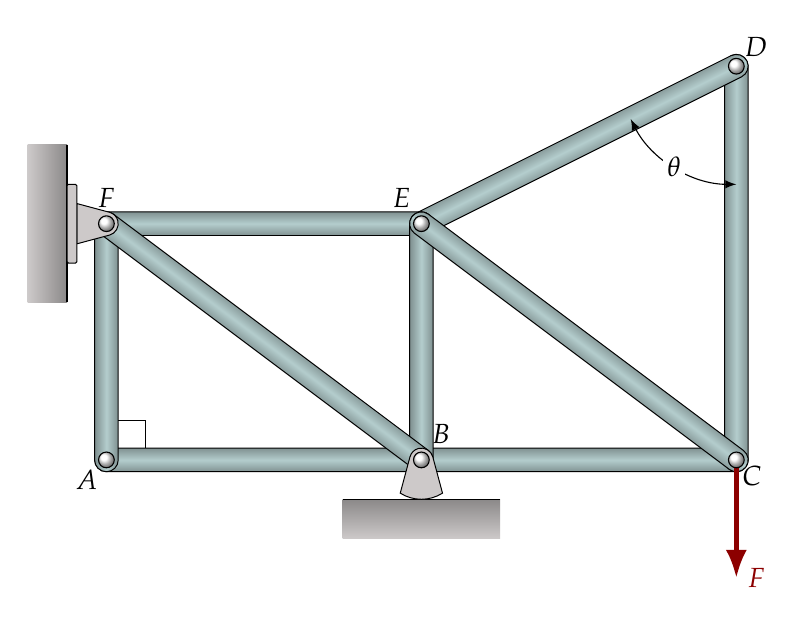
\begin{tikzpicture}[scale=\scale]
	\coordinate (A) at (0,0);
	\coordinate (B) at (4,0);
	\coordinate (C) at (8,0);
	\coordinate (D) at (8,5);
	\coordinate (E) at (4,3);
	\coordinate (F) at (0,3);

	\draw ($(A)+(0.5,0)$)--++(0,0.5)--+(-0.5,0);

	\Meme{A}{B}{LightCyan4}{LightCyan3}{black}{0.3}{0.15}{0.125}
	\Meme{C}{B}{LightCyan4}{LightCyan3}{black}{0.3}{0.15}{0.125}
	\Meme{C}{D}{LightCyan4}{LightCyan3}{black}{0.3}{0.15}{0.125}
	\Meme{E}{D}{LightCyan4}{LightCyan3}{black}{0.3}{0.15}{0.125}
	\Meme{E}{F}{LightCyan4}{LightCyan3}{black}{0.3}{0.15}{0.125}
	\Meme{A}{F}{LightCyan4}{LightCyan3}{black}{0.3}{0.15}{0.125}
	\Meme{B}{E}{LightCyan4}{LightCyan3}{black}{0.3}{0.15}{0.125}
	\Meme{C}{E}{LightCyan4}{LightCyan3}{black}{0.3}{0.15}{0.125}
	\Meme{B}{F}{LightCyan4}{LightCyan3}{black}{0.3}{0.15}{0.125}

	\fill[top color=Snow4, bottom color=Snow3]($(B)+(-1,-0.5)$)rectangle($(B)+(1,-1)$);
	\fill[right color=Snow4, left color=Snow3]($(F)+(-0.5,-1)$)rectangle($(F)+(-1,1)$);
	\draw($(B)+(-1,-0.5)$)--($(B)+(1,-0.5)$);
	\draw($(F)+(-0.5,1)$)--($(F)+(-0.5,-1)$);
	\PC[-90]{F}{Snow3}{black}{0.5}{0.125};
	\Rocker{B}{Snow3}{black}{0.5}{0.125};

	\draw[ultra thick, statsMaroon, -Latex] (C) -- ++ (0,-1.5) node[right]{$F$};

	\shadedraw [ball color = White] (A) circle (0.1cm) node[xshift=-0.25cm,yshift=-0.25cm] {$A$};
	\shadedraw [ball color = White] (B) circle (0.1cm) node[xshift=0.25cm,yshift=0.325cm] {$B$};
	\shadedraw [ball color = White] (C) circle (0.1cm) node[xshift=0.2cm,yshift=-0.2cm] {$C$};
	\shadedraw [ball color = White] (D) circle (0.1cm) node[xshift=0.25cm,yshift=0.25cm] {$D$};
	\shadedraw [ball color = White] (E) circle (0.1cm) node[xshift=-0.25cm,yshift=0.325cm] {$E$};
	\shadedraw [ball color = White] (F) circle (0.1cm) node[yshift=0.325cm] {$F$};

	\draw[latex-latex]($(D)+(206.57:1.5)$)arc(206.56:270:1.5)node[midway, fill=white, inner sep = 0.5mm]{$\theta$};

\end{tikzpicture}

		\end{statsbox}
	\end{textblock*}

	\begin{textblock*}{0.9\textwidth}(1.75cm, 6.5cm)
		There may be members in a truss that have no loading, as seen in the previous example.\par
		\textbf{Zero-force} members may be used to increase the stability of the truss during construction or to add support
		if the loading is changed.\par
		Identifying zero-force members can greatly simplify the analysis of a truss.
	\end{textblock*}
\end{frame}

%%%%%%%%%%%%%%%%%%%%%%%%%%%%%%%%%%%%%%%%%%%%%%%%%%%%%%%%%%%%%%%%%%%%%%%%%%%%%%%%%%%%%%%%%%%%%%%%%%%%


\begin{frame}{Zero-Force Members}
	\begin{textblock*}{0.65\textwidth}(0.875cm,2.25cm)
		\begin{statsbox}{}{}
			\centering
			\vbox to 4cm{
				\vfill
				\small
				\def\scale{0.55}
				

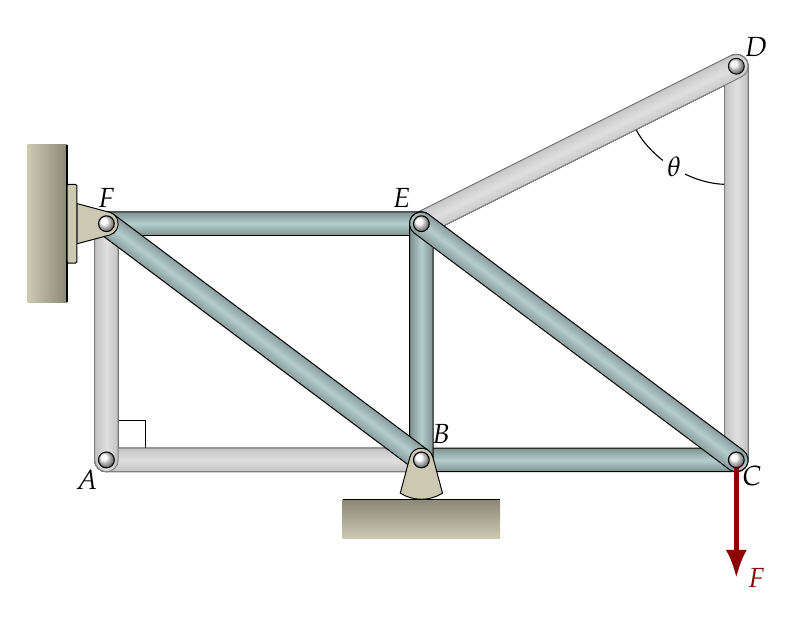
\begin{tikzpicture}[scale=\scale]
	\coordinate (A) at (0,0);
	\coordinate (B) at (4,0);
	\coordinate (C) at (8,0);
	\coordinate (D) at (8,5);
	\coordinate (E) at (4,3);
	\coordinate (F) at (0,3);

	\uncover<1>{
		\draw ($(A)+(0.5,0)$)--++(0,0.5)--+(-0.5,0);
		\Meme{A}{B}{LightCyan4}{LightCyan3}{black}{0.3}{0.15}{0.125}
		\Meme{A}{F}{LightCyan4}{LightCyan3}{black}{0.3}{0.15}{0.125}
	}
	\uncover<2-3>{
		\Meme{A}{B}{gray!50}{gray!25}{gray}{0.3}{0.15}{0.125}
		\Meme{A}{F}{gray!50}{gray!25}{gray}{0.3}{0.15}{0.125}
	}
	\Meme{C}{B}{LightCyan4}{LightCyan3}{black}{0.3}{0.15}{0.125}
	
	\uncover<1-2>{
		\Meme{C}{D}{LightCyan4}{LightCyan3}{black}{0.3}{0.15}{0.125}
		\Meme{E}{D}{LightCyan4}{LightCyan3}{black}{0.3}{0.15}{0.125}
		\draw[latex-latex]($(D)+(206.57:1.5)$)arc(206.56:270:1.5)node[midway, fill=white, inner sep = 0.5mm]{$\theta$};
	}
	\uncover<3>{
		\Meme{C}{D}{gray!50}{gray!25}{gray}{0.3}{0.15}{0.125}
		\Meme{E}{D}{gray!50}{gray!25}{gray}{0.3}{0.15}{0.125}
	}
	\Meme{E}{F}{LightCyan4}{LightCyan3}{black}{0.3}{0.15}{0.125}
	\Meme{E}{B}{LightCyan4}{LightCyan3}{black}{0.3}{0.15}{0.125}
	\Meme{E}{C}{LightCyan4}{LightCyan3}{black}{0.3}{0.15}{0.125}
	\Meme{B}{F}{LightCyan4}{LightCyan3}{black}{0.3}{0.15}{0.125}


	\fill[top color=Cornsilk4, bottom color=Cornsilk3]($(B)+(-1,-0.5)$)rectangle($(B)+(1,-1)$);
	\fill[right color=Cornsilk4, left color=Cornsilk3]($(F)+(-0.5,-1)$)rectangle($(F)+(-1,1)$);
	\draw($(B)+(-1,-0.5)$)--($(B)+(1,-0.5)$);
	\draw($(F)+(-0.5,1)$)--($(F)+(-0.5,-1)$);
	\PC[-90]{F}{Cornsilk3}{black}{0.5}{0.125};
	\Rocker{B}{Cornsilk3}{black}{0.5}{0.125};

	\draw[ultra thick, statsMaroon, -Latex] (C) -- ++ (0,-1.5) node[right]{$F$};

	\shadedraw [ball color = white] (B) circle (0.1cm) node[xshift=0.25cm,yshift=0.325cm] {$B$};
	\shadedraw [ball color = white] (C) circle (0.1cm) node[xshift=0.2cm,yshift=-0.2cm] {$C$};
	\shadedraw [ball color = white] (E) circle (0.1cm) node[xshift=-0.25cm,yshift=0.325cm] {$E$};
	\shadedraw [ball color = white] (F) circle (0.1cm) node[yshift=0.325cm] {$F$};

	\uncover<1>{
		\shadedraw [ball color = white] (A) circle (0.1cm) node[xshift=-0.25cm,yshift=-0.25cm] {$A$};
	}
	\uncover<2-3>{
		\shadedraw [ball color = gray!25, opacity=0.25] (A) circle (0.1cm);
	}
	\uncover<1-2>{
		\shadedraw [ball color = white] (D) circle (0.1cm) node[xshift=0.25cm,yshift=0.25cm] {$D$};
	}
	\uncover<3>{
		\shade [ball color = gray!25, opacity=0.25] (D) circle (0.1cm);
	}

\end{tikzpicture}

				\vfill
			}
		\end{statsbox}
	\end{textblock*}

	\begin{textblock*}{0.35\textwidth}(8.25cm, 1.875cm)
		\footnotesize
		\only<1-2>{
			\begin{statsbox}[adjusted title=Joint A]{}{}
				\centering
				\vbox to 4cm{
					\vfill
					\def\scale{0.75}
					\tikz[scale=\scale]{
						\coordinate (A) at (0,0);
						\draw[-latex, ultra thick] (A)--+(1.5,0)node[right]{$F_{AB}$};
						\draw[-latex, ultra thick] (A)--+(0,1.5)node[right]{$F_{AF}$};
						\fill[ball color=gray!50] (A) circle (3pt);
						\node[below left] (A){$A$};
					}
					\begin{align*}
						\Sigma F_x & = F_{AB} = 0 \\
						\Sigma F_y & = F_{AF} = 0 \\
					\end{align*}
					\uncover<2>{
						$AB$ and $AF$ are zero-force members.
					}
					\vfill
				}
			\end{statsbox}
		}
		\only<3->{
			\begin{statsbox}[adjusted title=Joint D]{}{}
				\centering
				\vbox to 4cm{
					\vfill
					\def\scale{0.75}
					\tikz[scale=\scale]{
						\coordinate (D) at (0,0);
						\draw[-latex, ultra thick] (D)--+(0,-1.75)node[left]{$F_{CD}$};
						\draw[-latex, ultra thick] (D)--+(206.565:1.75)node[above left]{$F_{DE}$};
						\fill[ball color=gray!50] (D) circle (3pt);
						\draw[latex-latex] ($(D)+(206.57:1.25)$)arc(206.57:270:1.25)node[midway,fill=white]{$\theta$};
						\node[above right] (D){$D$};
					}
					\begin{align*}
						\Sigma F_x         & = F_{DE}\sin\theta = 0 \\
						\Rightarrow F_{DE} & = 0                    \\
						\Sigma F_y         & = -F_{CD} = 0          \\
					\end{align*}
					\uncover<4>{
						$CD$ and $DE$ are zero-force members.
					}
					\vfill
				}
			\end{statsbox}
		}
	\end{textblock*}

	\begin{textblock*}{0.75\textwidth}(3cm, 7.75cm)
		\uncover<5>{
			\centering
			We can disregard all zero-force members and solve the simpler truss $BCEF$.
		}
	\end{textblock*}

\end{frame}

%%%%%%%%%%%%%%%%%%%%%%%%%%%%%%%%%%%%%%%%%%%%%%%%%%%%%%%%%%%%%%%%%%%%%%%%%%%%%%%%%%%%%%%%%%%%%%%%%%%%

\begin{frame}{Zero-Force Members}

	\begin{textblock*}{0.7\textwidth}(2.75cm, 1.375cm)
		\begin{statsbox}{}{}
			\centering
			\small
			\def\scale{0.55}
			% !TEX root = ../../Beamer/07MoJ/07MoJd.tex

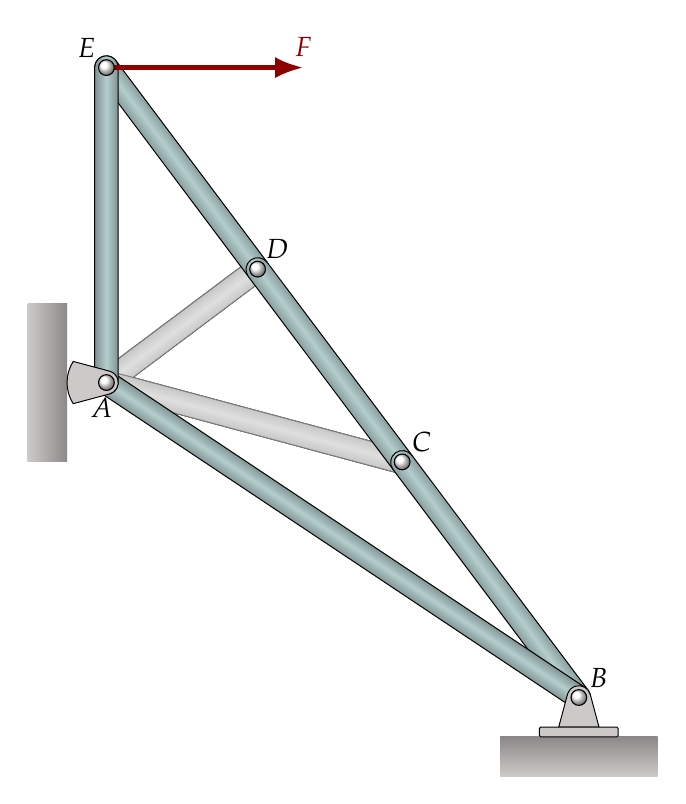
\begin{tikzpicture}[scale=\scale]
	\coordinate (A) at (0,0);
	\coordinate (B) at (6,-4);
	\coordinate (E) at (0,4);
	\coordinate (D) at ($(E)+(-53.13:3.2)$);
	\coordinate (C) at ($(D)!.45!(B)$);

	\uncover<1>{
		\Meme{A}{D}{LightCyan4}{LightCyan3}{black}{0.3}{0.15}{0.125}
	}
	\uncover<1-2>{
		\Meme{A}{C}{LightCyan4}{LightCyan3}{black}{0.3}{0.15}{0.125}
	}
	\uncover<2->{
		\Meme{A}{D}{gray!50}{gray!25}{gray}{0.3}{0.15}{0.125}
	}
	\uncover<3>{
		\Meme{A}{C}{gray!50}{gray!25}{gray}{0.3}{0.15}{0.125}
	}

	\Meme{E}{D}{LightCyan4}{LightCyan3}{black}{0.3}{0.15}{0.125}
	\Meme{C}{D}{LightCyan4}{LightCyan3}{black}{0.3}{0.15}{0.125}
	\Meme{B}{C}{LightCyan4}{LightCyan3}{black}{0.3}{0.15}{0.125}
	\Meme{A}{B}{LightCyan4}{LightCyan3}{black}{0.3}{0.15}{0.125}
	\Meme{A}{E}{LightCyan4}{LightCyan3}{black}{0.3}{0.15}{0.125}	

	\fill[top color=Snow4, bottom color=Snow3]($(B)+(-1,-0.5)$)rectangle($(B)+(1,-1)$);
	\fill[right color=Snow4, left color=Snow3]($(A)+(-0.5,-1)$)rectangle($(A)+(-1,1)$);
	\PC{B}{Snow3}{black}{0.5}{0.125};
	\Rocker[270]{A}{Snow3}{black}{0.5}{0.125};

	\draw[ultra thick, statsMaroon, -Latex] (E) -- ++ (2.5,0) node[above]{$F$};

	\shadedraw [ball color = white] (A) circle (0.1cm) node[xshift=-0.0625cm,yshift=-0.325cm] {$A$};
	\shadedraw [ball color = white] (B) circle (0.1cm) node[xshift=0.25cm,yshift=0.25cm] {$B$};
	\shadedraw [ball color = white] (C) circle (0.1cm) node[xshift=0.25cm,yshift=0.25cm] {$C$};
	\shadedraw [ball color = white] (D) circle (0.1cm) node[xshift=0.25cm,yshift=0.25cm] {$D$};
	\shadedraw [ball color = white] (E) circle (0.1cm) node[xshift=-0.25cm,yshift=0.25cm] {$E$};

\end{tikzpicture}

		\end{statsbox}
	\end{textblock*}

	\begin{textblock*}{0.7\textwidth}(2.875cm, 8.0cm)
		\centering
		\uncover<1->{
			Truss members $BC$, $CD$ and $DE$ are collinear.\lb
			Are there any zero-force members?	\parm
		}
		\uncover<2->{
			$AD$ is a zero-force member.\lb
		}
		\uncover<3>{
			So is $AC$.
		}
	\end{textblock*}

\end{frame}

%%%%%%%%%%%%%%%%%%%%%%%%%%%%%%%%%%%%%%%%%%%%%%%%%%%%%%%%%%%%%%%%%%%%%%%%%%%%%%%%%%%%%%%%%%%%%%%%%%%%

\begin{frame}{Zero-Force Members}

	\begin{textblock*}{0.45\textwidth}(1.25cm, 1.375cm)
		\begin{statsbox}{}{}
			\centering
			\small
			\def\scale{0.35}
			% !TEX root = ../../Beamer/07MoJ/07MoJd.tex

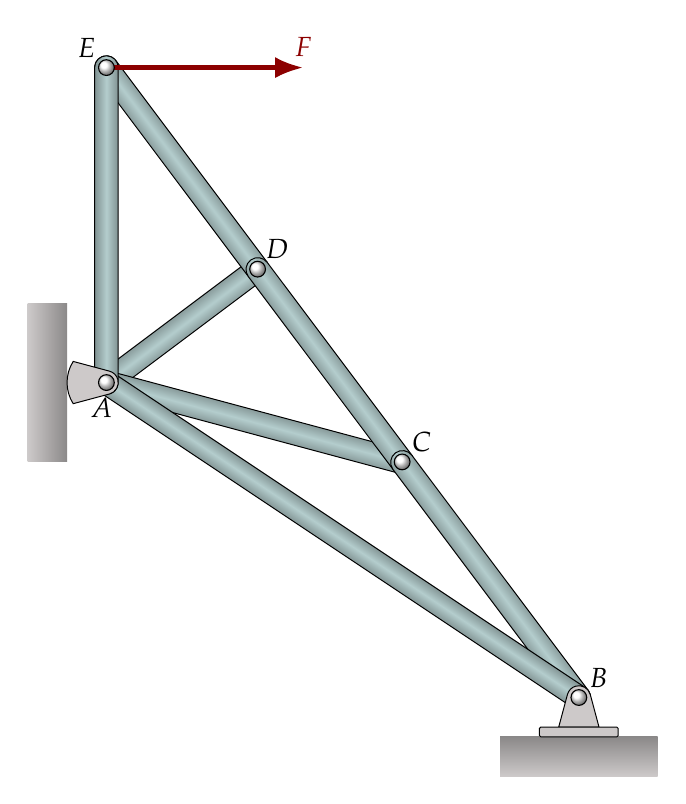
\begin{tikzpicture}[scale=\scale]
	\coordinate (A) at (0,0);
	\coordinate (B) at (6,-4);
	\coordinate (E) at (0,4);
	\coordinate (D) at ($(E)+(-53.13:3.2)$);
	\coordinate (C) at ($(D)!.45!(B)$);


	\Meme{A}{D}{LightCyan4}{LightCyan3}{black}{0.3}{0.15}{0.125}
	\Meme{A}{C}{LightCyan4}{LightCyan3}{black}{0.3}{0.15}{0.125}
	\Meme{E}{D}{LightCyan4}{LightCyan3}{black}{0.3}{0.15}{0.125}
	\Meme{C}{D}{LightCyan4}{LightCyan3}{black}{0.3}{0.15}{0.125}
	\Meme{B}{C}{LightCyan4}{LightCyan3}{black}{0.3}{0.15}{0.125}
	\Meme{A}{B}{LightCyan4}{LightCyan3}{black}{0.3}{0.15}{0.125}
	\Meme{A}{E}{LightCyan4}{LightCyan3}{black}{0.3}{0.15}{0.125}	

	\fill[top color=Snow4, bottom color=Snow3]($(B)+(-1,-0.5)$)rectangle($(B)+(1,-1)$);
	\fill[right color=Snow4, left color=Snow3]($(A)+(-0.5,-1)$)rectangle($(A)+(-1,1)$);
	\PC{B}{Snow3}{black}{0.5}{0.125};
	\Rocker[270]{A}{Snow3}{black}{0.5}{0.125};

	\draw[ultra thick, statsMaroon, -Latex] (E) -- ++ (2.5,0) node[above]{$F$};

	\shadedraw [ball color = white] (A) circle (0.1cm) node[xshift=-0.0625cm,yshift=-0.325cm] {$A$};
	\shadedraw [ball color = white] (B) circle (0.1cm) node[xshift=0.25cm,yshift=0.25cm] {$B$};
	\shadedraw [ball color = white] (C) circle (0.1cm) node[xshift=0.25cm,yshift=0.25cm] {$C$};
	\shadedraw [ball color = white] (D) circle (0.1cm) node[xshift=0.25cm,yshift=0.25cm] {$D$};
	\shadedraw [ball color = white] (E) circle (0.1cm) node[xshift=-0.25cm,yshift=0.25cm] {$E$};

\end{tikzpicture}

		\end{statsbox}
	\end{textblock*}

	\begin{textblock*}{0.45\textwidth}(6.75cm, 1.375cm)
		\begin{statsbox}{}{}
			\centering
			\small
			\def\scale{0.35}
			% !TEX root = ../../Beamer/07MoJ/07MoJd.tex

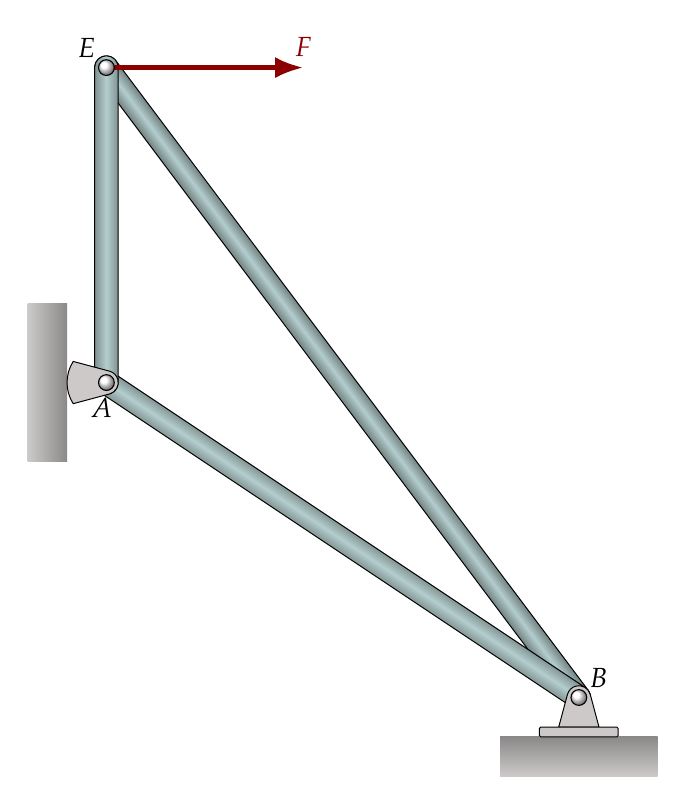
\begin{tikzpicture}[scale=\scale]
	\coordinate (A) at (0,0);
	\coordinate (B) at (6,-4);
	\coordinate (E) at (0,4);
	\coordinate (D) at ($(E)+(-53.13:3.2)$);
	\coordinate (C) at ($(D)!.45!(B)$);


	
	
	\Meme{B}{E}{LightCyan4}{LightCyan3}{black}{0.3}{0.15}{0.125}	
	\Meme{A}{B}{LightCyan4}{LightCyan3}{black}{0.3}{0.15}{0.125}
	\Meme{A}{E}{LightCyan4}{LightCyan3}{black}{0.3}{0.15}{0.125}	

	\fill[top color=Snow4, bottom color=Snow3]($(B)+(-1,-0.5)$)rectangle($(B)+(1,-1)$);
	\fill[right color=Snow4, left color=Snow3]($(A)+(-0.5,-1)$)rectangle($(A)+(-1,1)$);
	\PC{B}{Snow3}{black}{0.5}{0.125};
	\Rocker[270]{A}{Snow3}{black}{0.5}{0.125};

	\draw[ultra thick, statsMaroon, -Latex] (E) -- ++ (2.5,0) node[above]{$F$};

	\shadedraw [ball color = white] (A) circle (0.1cm) node[xshift=-0.0625cm,yshift=-0.325cm] {$A$};
	\shadedraw [ball color = white] (B) circle (0.1cm) node[xshift=0.25cm,yshift=0.25cm] {$B$};
	\shadedraw [ball color = white] (E) circle (0.1cm) node[xshift=-0.25cm,yshift=0.25cm] {$E$};

\end{tikzpicture}

		\end{statsbox}
	\end{textblock*}

	\begin{textblock*}{1\textwidth}(1cm, 6.25cm)
		\raggedright
		% \footnotesize
	If $AC$ and $D$ are zero-force members, why not just omit them altogether and have a single member from $B$ to $E$? \par
		\uncover<2->{
		Of course, all designs are different, but $BE$ is long and slender, and the force $F$ will put it in compression. If the load is too high, $BE$ will buckle. (You will learn about the buckling of columns in your strength of materials course.) \par 
		}\uncover<3> {Braces at $C$ and $D$ can increase the load before buckling by up to nine times.		}
	
	\end{textblock*}

\end{frame}

%%%%%%%%%%%%%%%%%%%%%%%%%%%%%%%%%%%%%%%%%%%%%%%%%%%%%%%%%%%%%%%%%%%%%%%%%%%%%%%%%%%%%%%%%%%%%%%%%%%%

\begin{frame}{}

	\begin{textblock*}{0.85\textwidth}(2cm, 0.375cm)
		\begin{statsbox}[title=Zero-Force Members]{}{}
			\centering
			\small
			\def\scale{0.55}
			% !TEX root = ../../Beamer/07MoJ/07MoJd.tex

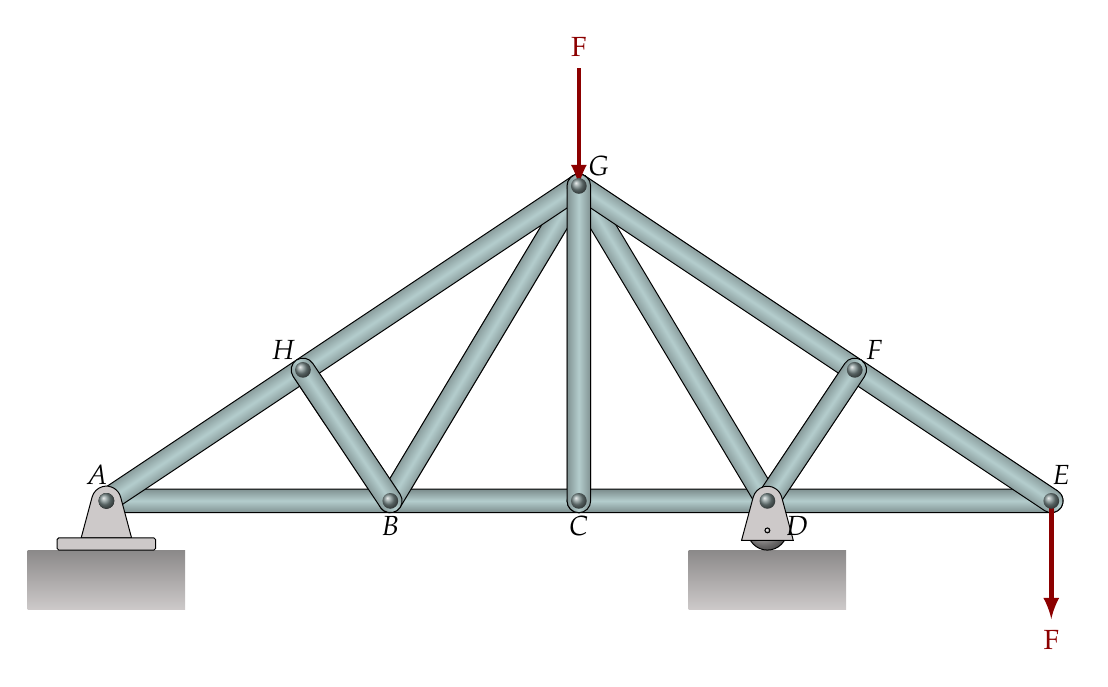
\begin{tikzpicture}[scale=\scale]
	\coordinate (A) at (-6,0);
	\coordinate (B) at (-2.3945,0);
	\coordinate (C) at (0,0);
	\coordinate (D) at (2.3945,0);
	\coordinate (E) at (6,0);
	\coordinate (G) at (0,4);
	\coordinate (H) at ($(A)+(33.69:3)$);
	\coordinate (F) at ($(E)+(146.31:3)$);

	\uncover<2->{
		\Meme{B}{H}{gray!50}{gray!25}{gray}{0.3}{0.15}{0.125}
		\Meme{D}{F}{gray!50}{gray!25}{gray}{0.3}{0.15}{0.125}
		\Meme{C}{G}{gray!50}{gray!25}{gray}{0.3}{0.15}{0.125}
	}
	\uncover<3->{
		\Meme{B}{G}{gray!50}{gray!25}{gray}{0.3}{0.15}{0.125}
	}

	\Meme{A}{B}{LightCyan4}{LightCyan3}{black}{0.3}{0.15}{0.125}
	\Meme{C}{B}{LightCyan4}{LightCyan3}{black}{0.3}{0.15}{0.125}
	\Meme{C}{D}{LightCyan4}{LightCyan3}{black}{0.3}{0.15}{0.125}
	\Meme{E}{D}{LightCyan4}{LightCyan3}{black}{0.3}{0.15}{0.125}
	\Meme{G}{D}{LightCyan4}{LightCyan3}{black}{0.3}{0.15}{0.125}
	\Meme{A}{H}{LightCyan4}{LightCyan3}{black}{0.3}{0.15}{0.125}
	
	\uncover<1-2>{
		\Meme{G}{B}{LightCyan4}{LightCyan3}{black}{0.3}{0.15}{0.125}
	}
	\Meme{G}{H}{LightCyan4}{LightCyan3}{black}{0.3}{0.15}{0.125}
	\Meme{E}{F}{LightCyan4}{LightCyan3}{black}{0.3}{0.15}{0.125}
	\Meme{G}{F}{LightCyan4}{LightCyan3}{black}{0.3}{0.15}{0.125}

	\uncover<1>{
		\Meme{B}{H}{LightCyan4}{LightCyan3}{black}{0.3}{0.15}{0.125}
		\Meme{D}{F}{LightCyan4}{LightCyan3}{black}{0.3}{0.15}{0.125}
		\Meme{C}{G}{LightCyan4}{LightCyan3}{black}{0.3}{0.15}{0.125}
	}

	\fill[top color=Snow4, bottom color=Snow3]($(D)+(-1,-0.625)$)rectangle($(D)+(1,-1.375)$);
	\fill[top color=Snow4, bottom color=Snow3]($(A)+(-1,-0.625)$)rectangle($(A)+(1,-1.375)$);
	\PC{A}{Snow3}{black}{0.625}{0.125};
	\Rone{D}{Snow3}{black}{0.625}{0.125};
	%
	\draw[ultra thick, saitMaroon, -latex] (E) -- ++ (0,-1.5) node[below]{$\mathrm{\bm F}$};
	\draw[ultra thick, saitMaroon, latex-] (G) -- ++ (0,1.5) node[above]{$\mathrm{\bm F}$};
	%
	\shade [ball color = LightCyan4] (A) circle (0.1cm) node[xshift=-0.125cm, yshift=0.325cm] {$A$};
	\shade [ball color = LightCyan4] (B) circle (0.1cm) node[yshift=-0.325cm] {$B$};
	\shade [ball color = LightCyan4] (C) circle (0.1cm) node[yshift=-0.325cm] {$C$};
	\shade [ball color = LightCyan4] (D) circle (0.1cm) node[xshift=0.375cm, yshift=-0.315cm] {$D$};
	\shade [ball color = LightCyan4] (E) circle (0.1cm) node[xshift=0.125cm,yshift=0.325cm] {$E$};
	\shade [ball color = LightCyan4] (F) circle (0.1cm) node[xshift=0.25cm, yshift=0.25cm] {$F$};
	\shade [ball color = LightCyan4] (G) circle (0.1cm) node[xshift=0.25cm, yshift=0.25cm] {$G$};
	\shade [ball color = LightCyan4] (H) circle (0.1cm) node[xshift=-0.25cm, yshift=0.25cm] {$H$};

\end{tikzpicture}

		\end{statsbox}
	\end{textblock*}

	\begin{textblock*}{0.7\textwidth}(2.875cm, 6.5cm)
		\centering
		\uncover<1->{
			Truss members $BC$, $CD$ and $DE$ are collinear.\lb
			Are there any zero-force members?	\parm
		}
		\uncover<2->{
			$BH$, $CG$ and $DF$ are zero-force members.\lb
		}
		\uncover<3>{
			So is $BG$ (because $BH$ is a zero-force member).
		}
	\end{textblock*}

\end{frame}

%%%%%%%%%%%%%%%%%%%%%%%%%%%%%%%%%%%%%%%%%%%%%%%%%%%%%%%%%%%%%%%%%%%%%%%%%%%%%%%%%%%%%%%%%%%%%%%%%%%%

\begin{frame}{}

	\begin{textblock*}{0.85\textwidth}(2cm, 0.375cm)
		\begin{statsbox}[title=Zero-Force Members]{}{}
			\centering
			\small
			\def\scale{0.65}
			% !TEX root = ../../Beamer/07MoJ/07MoJd.tex

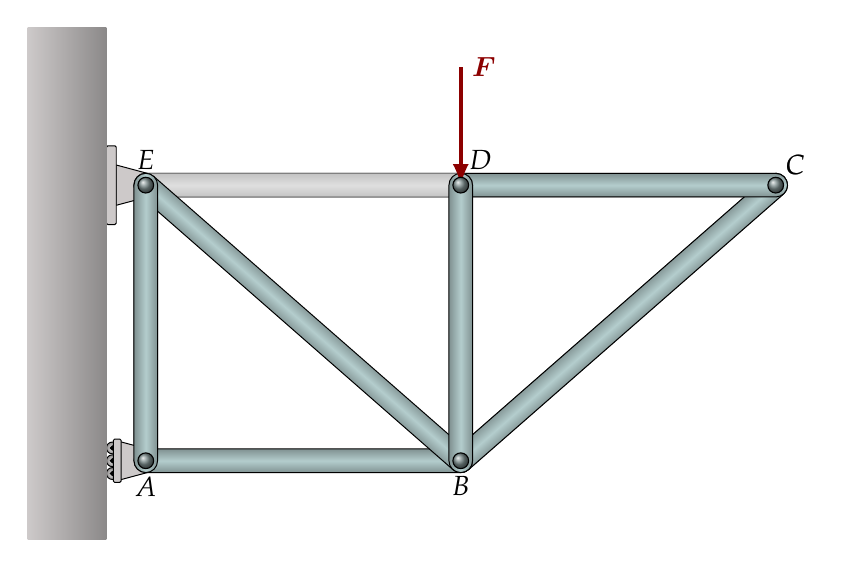
\begin{tikzpicture}[scale=\scale]

	\coordinate (A) at (0,0);
	\coordinate (B) at (4,0);
	\coordinate (E) at (0,3.5);
	\coordinate (D) at (4,3.5);
	\coordinate (C) at (8,3.5);



	\uncover<4>{
		\Meme{A}{E}{gray!50}{gray!25}{gray}{0.3}{0.15}{0.125}
	}

	\PC[-90]{E}{Snow3}{black}{0.5}{0.125};
	\Roller[-90]{A}{Snow3}{black}{0.5}{0.125};
	\fill[right color=Snow4, left color=Snow3]($(A)+(-0.5,-1)$)rectangle($(E)+(-1.5,2)$);

	\uncover<2->{
		\Meme{B}{C}{gray!50}{gray!25}{gray}{0.3}{0.15}{0.125}
		\Meme{D}{C}{gray!50}{gray!25}{gray}{0.3}{0.15}{0.125}
		\shade [ball color = gray!20] (C) circle (0.1cm);
		\shadedraw [ball color = gray, opacity = 0.5] (C) circle (0.1cm) node[xshift=0.25cm, yshift=0.25cm] {$C$};
	}
	\Meme{A}{B}{LightCyan4}{LightCyan3}{black}{0.3}{0.15}{0.125}
	\uncover<1>{
		\Meme{B}{C}{LightCyan4}{LightCyan3}{black}{0.3}{0.15}{0.125}
		\Meme{D}{C}{LightCyan4}{LightCyan3}{black}{0.3}{0.15}{0.125}
		\shadedraw [ball color = LightCyan4] (C) circle (0.1cm) node[xshift=0.25cm, yshift=0.25cm] {$C$};
	}
	\uncover<1-2>{
		\Meme{E}{D}{LightCyan4}{LightCyan3}{black}{0.3}{0.15}{0.125}
	}
	\uncover<3->{
		\Meme{E}{D}{gray!50}{gray!25}{gray}{0.3}{0.15}{0.125}
	}
	
	\Meme{E}{B}{LightCyan4}{LightCyan3}{black}{0.3}{0.15}{0.125}
	\Meme{D}{B}{LightCyan4}{LightCyan3}{black}{0.3}{0.15}{0.125}
	\uncover<1-3>{
		\Meme{E}{A}{LightCyan4}{LightCyan3}{black}{0.3}{0.15}{0.125}
	}

	\draw[ultra thick, saitMaroon, latex-] (D) -- ++ (0,1.5) node[right]{$\bm F$};

	\shadedraw [ball color = LightCyan4,thin] (A) circle (0.1cm) node[yshift=-0.325cm] {$A$};
	\shadedraw [ball color = LightCyan4] (B) circle (0.1cm) node[yshift=-0.325cm] {$B$};
	\shadedraw [ball color = LightCyan4] (D) circle (0.1cm) node[xshift=0.25cm, yshift=0.325cm] {$D$};
	\shadedraw [ball color = LightCyan4] (E) circle (0.1cm) node[yshift=0.325cm] {$E$};

\end{tikzpicture}

		\end{statsbox}
	\end{textblock*}

	\begin{textblock*}{0.7\textwidth}(2.875cm, 5.75cm)
		\centering
		\uncover<1->{
			Are there any zero-force members?	\parm
		}
		\uncover<2->{
			$BC$ and $CD$ are zero-force members.\lb
		}
		\uncover<3->{
			$DE$ is a zero-force member -- because $CD$ is.\lb
			Are there any more? \lb
		}
		\uncover<4->{
			$AE$ is a zero-force member.
		}
	\end{textblock*}

\end{frame}

%%%%%%%%%%%%%%%%%%%%%%%%%%%%%%%%%%%%%%%%%%%%%%%%%%%%%%%%%%%%%%%%%%%%%%%%%%%%%%%%%%%%%%%%%%%%%%%%%%%%%%%%%%%%%%%%%%%%%%%%%%%%%%%

\begin{frame}{}
	\begin{myexam}{}{}
		\def\scale{0.65}
		\centering
		%%%%%%%%%%%%%%%%%%%%%%% TRUSS %%%%%%%%%%%%%%%%%%%%%%%%%%%%%%%%%%%%%%%%%%%%%%%%%%%%%%%%%%%%%%%%%%%%%
% !TEX root = ../../Beamer/07MoJ/07MoJ.tex

%http://tex.stackexchange.com/questions/33703/extract-x-y-coordinate-of-an-arbitrary-point-in-tikz
\makeatletter
\providecommand{\gettikzxy}[3]{%
	\tikz@scan@one@point\pgfutil@firstofone#1\relax
	\edef#2{\the\pgf@x}%
	\edef#3{\the\pgf@y}%
}
\makeatother

%%%%%%%%%%%%%%%%%%%%%%% TRUSS %%%%%%%%%%%%%%%%%%%%%%%%%%%%%%%%%%%%%%%%%%%%%%%%%%%%%%%%%%%%%%%%%%%%%


%%%%%%%%%%%%%%%%%%%%%%% TRUSS %%%%%%%%%%%%%%%%%%%%%%%%%%%%%%%%%%%%%%%%%%%%%%%%%%%%%%%%%%%%%%%%%%%%%
\begin{tikzpicture}[scale=\scale]

	\coordinate (A) at (0,0);
	\coordinate (B)	at (2,0);
	\coordinate (C) at (4,0);
	\coordinate (D) at (6,0);
	\coordinate (E) at (8,0);
	\coordinate (F) at (10,0);
	\coordinate (G) at (12,0);
	\coordinate (H) at (10,1.5);
	\coordinate (I) at (8,3);
	\coordinate (J) at (6,4.5);
	\coordinate (K) at (4,3);
	\coordinate (L) at (2,1.5);
	\footnotesize
	\PinnedConnection{A}{Honeydew3}{black}{0.5}{0.125}
	\Rocker{G}{Honeydew3}{black}{0.5}{0.125}

	% \filldraw[fill=Cornsilk2] ($(DD)+(25:2.5)$)--++(205:2.5)--+(2.25,0);
	% \draw[latex-latex] ($(DD)+(25:1.75)$)arc(25:0:1.75)node[fill=Cornsilk2, midway, inner sep=0.5mm]{$25\degree$};
	\fill[top color=Honeydew4,bottom color=Honeydew2] ($(A)+(-1,-0.5)$)rectangle($(A)+(1,-1)$);
	\fill[top color=Honeydew4,bottom color=Honeydew2] ($(G)+(-1,-0.5)$)rectangle($(G)+(1,-1)$);
	\draw ($(A)+(-1,-0.5)$)--($(A)+(1,-0.5)$);
	\draw ($(G)+(-1,-0.5)$)--($(G)+(1,-0.5)$);

	\pgfoonew \BL=new rrect(B,L,DarkOrchid4,DarkOrchid1,black,0.3,0.3,0.3,0.125);
	\pgfoonew \CK=new rrect(C,K,DarkOrchid4,DarkOrchid1,black,0.3,0.3,0.3,0.125);
	\pgfoonew \DJ=new rrect(D,J,DarkOrchid4,DarkOrchid1,black,0.3,0.3,0.3,0.125);
	\pgfoonew \EI=new rrect(E,I,DarkOrchid4,DarkOrchid1,black,0.3,0.3,0.3,0.125);
	\pgfoonew \FH=new rrect(F,H,DarkOrchid4,DarkOrchid1,black,0.3,0.3,0.3,0.125);
	\pgfoonew \CL=new rrect(C,L,DarkOrchid4,DarkOrchid1,black,0.3,0.3,0.3,0.125);
	\pgfoonew \DK=new rrect(D,K,DarkOrchid4,DarkOrchid1,black,0.3,0.3,0.3,0.125);
	\pgfoonew \DI=new rrect(D,I,DarkOrchid4,DarkOrchid1,black,0.3,0.3,0.3,0.125);
	\pgfoonew \EH=new rrect(E,H,DarkOrchid4,DarkOrchid1,black,0.3,0.3,0.3,0.125);
	\pgfoonew \AB=new rrect(B,A,DarkOrchid4,DarkOrchid1,black,0.3,0.3,0.3,0.125);
	\pgfoonew \BC=new rrect(B,C,DarkOrchid4,DarkOrchid1,black,0.3,0.3,0.3,0.125);
	\pgfoonew \CD=new rrect(C,D,DarkOrchid4,DarkOrchid1,black,0.3,0.3,0.3,0.125);
	\pgfoonew \DE=new rrect(D,E,DarkOrchid4,DarkOrchid1,black,0.3,0.3,0.3,0.125);
	\pgfoonew \EF=new rrect(E,F,DarkOrchid4,DarkOrchid1,black,0.3,0.3,0.3,0.125);
	\pgfoonew \FG=new rrect(F,G,DarkOrchid4,DarkOrchid1,black,0.3,0.3,0.3,0.125);
	\pgfoonew \AL=new rrect(A,L,DarkOrchid4,DarkOrchid1,black,0.3,0.3,0.3,0.125);
	\pgfoonew \LK=new rrect(L,K,DarkOrchid4,DarkOrchid1,black,0.3,0.3,0.3,0.125);
	\pgfoonew \KJ=new rrect(K,J,DarkOrchid4,DarkOrchid1,black,0.3,0.3,0.3,0.125);
	\pgfoonew \GH=new rrect(G,H,DarkOrchid4,DarkOrchid1,black,0.3,0.3,0.3,0.125);
	\pgfoonew \IH=new rrect(I,H,DarkOrchid4,DarkOrchid1,black,0.3,0.3,0.3,0.125);
	\pgfoonew \JI=new rrect(J,I,DarkOrchid4,DarkOrchid1,black,0.3,0.3,0.3,0.125);



	\draw[ultra thick, saitMaroon, -Latex] (D)--+(0,-2.75)node[below,black]{$12.0\,$kN};
	\draw[ultra thick, saitMaroon, -Latex] (C)--+(0,-2.25)node[below,black]{$10.0\,$kN};
	\draw[ultra thick, saitMaroon, -Latex] (E)--+(0,-2.25)node[below,black]{$10.0\,$kN};
	% \draw[ultra thick, saitDeepBlue, -Latex] (A)--+(2,0)node[right,black]{$2.00\,$kN};
	%
	\shadedraw[ball color=Azure3, draw=black] (A) circle (2.5pt)node[xshift=-0.125cm, yshift=0.25cm]{\normalsize $A$};
	\shadedraw[ball color=Azure3, draw=black] (B) circle (2.5pt)node[xshift=0.2cm, yshift=-0.3cm]{\normalsize $B$};
	\shadedraw[ball color=Azure3, draw=black] (C) circle (2.5pt)node[xshift=0.2cm, yshift=-0.3cm]{\normalsize $C$};
	\shadedraw[ball color=Azure3, draw=black] (D) circle (2.5pt)node[xshift=0.2cm, yshift=-0.3cm]{\normalsize $D$};
	\shadedraw[ball color=Azure3, draw=black] (E) circle (2.5pt)node[xshift=0.2cm, yshift=-0.3cm]{\normalsize $E$};
	\shadedraw[ball color=Azure3, draw=black] (F) circle (2.5pt)node[xshift=0.2cm, yshift=-0.3cm]{\normalsize $F$};
	\shadedraw[ball color=Azure3, draw=black] (G) circle (2.5pt)node[yshift=0.35cm]{\normalsize $G$};
	\shadedraw[ball color=Azure3, draw=black] (H) circle (2.5pt)node[yshift=0.35cm]{\normalsize $H$};
	\shadedraw[ball color=Azure3, draw=black] (H) circle (2.5pt)node[yshift=0.35cm]{\normalsize $H$};
	\shadedraw[ball color=Azure3, draw=black] (I) circle (2.5pt)node[yshift=0.35cm]{\normalsize $I$};
	\shadedraw[ball color=Azure3, draw=black] (J) circle (2.5pt)node[yshift=0.35cm]{\normalsize $J$};
	\shadedraw[ball color=Azure3, draw=black] (K) circle (2.5pt)node[yshift=0.35cm]{\normalsize $K$};
	\shadedraw[ball color=Azure3, draw=black] (L) circle (2.5pt)node[yshift=0.35cm]{\normalsize $L$};
	%
	\draw[thin] ($(A)+(-0.5,0)$)--+(-1,0);
	\draw[thin] ($(L)+(-0.5,0)$)--+(-3,0);
	\draw[thin] ($(K)+(-0.5,0)$)--+(-5,0);
	\draw[thin] ($(J)+(-0.5,0)$)--+(-7,0);
	\draw[thin] ($(A)+(0,-0.25)$)--+(0,-1.25);
	\draw[thin] ($(B)+(0,-0.25)$)--+(0,-1.25);
	\draw[thin] ($(F)+(0,-0.25)$)--+(0,-1.25);
	\draw[thin] ($(G)+(0,-0.25)$)--+(0,-1.25);
	% % \draw[thin] ($(B)+(-0.25,0)$)--+(-1,0);
	% \draw[thin] ($(A)+(-0.25,0)$)--+(-1,0);
	\draw[latex-latex] ($(A)+(0,-1.25)$)--node[fill=white,inner sep=0.25mm]{$1.50\,$m}($(B)+(0,-1.25)$);
	\draw[latex-latex] ($(B)+(0,-1.25)$)--node[fill=white,inner sep=0.25mm]{$1.50\,$m}($(C)+(0,-1.25)$);
	\draw[latex-latex] ($(C)+(0,-1.25)$)--node[fill=white,inner sep=0.25mm]{$1.50\,$m}($(D)+(0,-1.25)$);
	\draw[latex-latex] ($(D)+(0,-1.25)$)--node[fill=white,inner sep=0.25mm]{$1.50\,$m}($(E)+(0,-1.25)$);
	\draw[latex-latex] ($(E)+(0,-1.25)$)--node[fill=white,inner sep=0.25mm]{$1.50\,$m}($(F)+(0,-1.25)$);
	\draw[latex-latex] ($(F)+(0,-1.25)$)--node[fill=white,inner sep=0.25mm]{$1.50\,$m}($(G)+(0,-1.25)$);
	\draw[latex-latex] ($(A)+(-1,0)$)--node[fill=white]{$1.15\,$m}($(L)+(-3,0)$);
	\draw[latex-latex] ($(L)+(-3,0)$)--node[fill=white]{$1.15\,$m}($(K)+(-5,0)$);
	\draw[latex-latex] ($(K)+(-5,0)$)--node[fill=white]{$1.15\,$m}($(J)+(-7,0)$);
	% \draw[latex-latex] ($(A)+(0,-0.75)$)--node[fill=white]{$1210\,$mm}($(B)+(0,-0.75)$);
	% \draw[latex-latex] ($(B)+(0,-0.75)$)--node[fill=white]{$1210\,$mm}($(C)+(0,-0.75)$);
	% \draw[latex-latex] ($(C)+(0,-1.25)$)--node[fill=white]{$2.10\,$m}($(D)+(0,-1.25)$);
	% \draw[latex-latex] ($(B)+(-0.75,0)$)--node[fill=white]{$1.65\,$m}($(A)+(-4.75,0)$);


	%
\end{tikzpicture}

		\cmini[0.65]{
			\centering
			Determine the force in each truss member.
		}
	\end{myexam}
\end{frame}

%%%%%%%%%%%%%%%%%%%%%%%%%%%%%%%%%%%%%%%%%%%%%%%%%%%%%%%%%%%%%%%%%%%%%%%%%%%%%%%%%%%%%%%%%%%%%%%%%%%%

\begin{frame}{Types of Forces}
	\small\centering\vspace{0.25cm}
	\def\scale{0.75}
	%%%%%%%%%%%%%%%%%%%%%%% TRUSS %%%%%%%%%%%%%%%%%%%%%%%%%%%%%%%%%%%%%%%%%%%%%%%%%%%%%%%%%%%%%%%%%%%%%
% !TEX root = ../../Beamer/07MoJ/07MoJ.tex

%http://tex.stackexchange.com/questions/33703/extract-x-y-coordinate-of-an-arbitrary-point-in-tikz
\makeatletter
\providecommand{\gettikzxy}[3]{%
	\tikz@scan@one@point\pgfutil@firstofone#1\relax
	\edef#2{\the\pgf@x}%
	\edef#3{\the\pgf@y}%
}
\makeatother

%%%%%%%%%%%%%%%%%%%%%%% TRUSS %%%%%%%%%%%%%%%%%%%%%%%%%%%%%%%%%%%%%%%%%%%%%%%%%%%%%%%%%%%%%%%%%%%%%


%%%%%%%%%%%%%%%%%%%%%%% TRUSS %%%%%%%%%%%%%%%%%%%%%%%%%%%%%%%%%%%%%%%%%%%%%%%%%%%%%%%%%%%%%%%%%%%%%
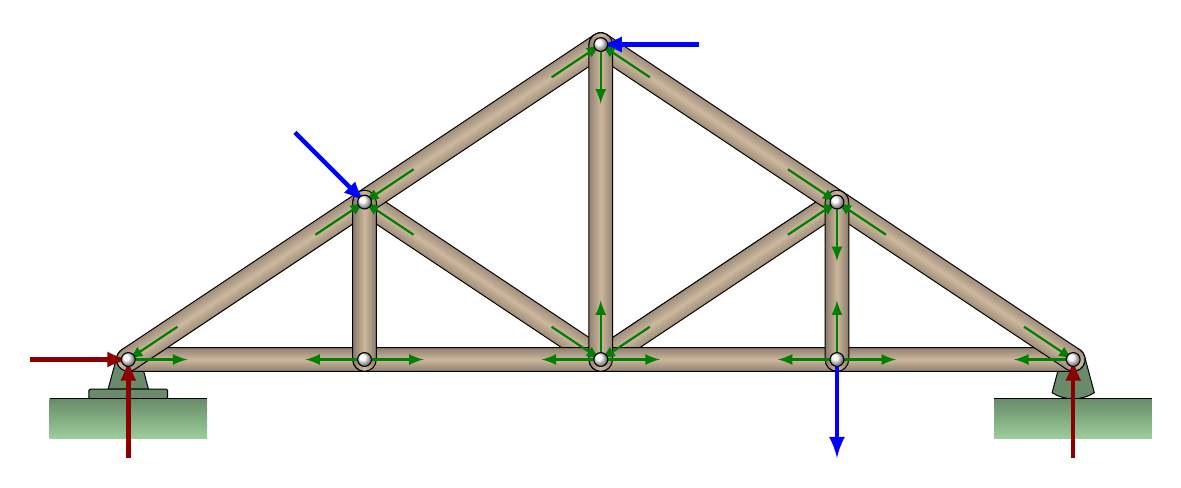
\begin{tikzpicture}[scale=\scale]

	\coordinate (A) at (0,0);
	\coordinate (B)	at (3,0);
	\coordinate (C) at (6,0);
	\coordinate (D) at (9,0);
	\coordinate (E) at (12,0);
	\coordinate (F) at (9,2);
	\coordinate (G) at (6,4);
	\coordinate (H) at (3,2);
	\footnotesize
	\PC{A}{DarkSeaGreen4}{black}{0.5}{0.125}
	\Rocker{E}{DarkSeaGreen4}{black}{0.5}{0.125}

	\fill[top color=DarkSeaGreen4,bottom color=DarkSeaGreen3] ($(A)+(-1,-0.5)$)rectangle($(A)+(1,-1)$);
	\fill[top color=DarkSeaGreen4,bottom color=DarkSeaGreen3] ($(E)+(-1,-0.5)$)rectangle($(E)+(1,-1)$);
	\draw ($(A)+(-1,-0.5)$)--($(A)+(1,-0.5)$);
	\draw ($(E)+(-1,-0.5)$)--($(E)+(1,-0.5)$);

	\Meme{C}{F}{Bisque4}{Bisque3}{black}{0.3}{0.15}{0.125}
	\Meme{C}{H}{Bisque4}{Bisque3}{black}{0.3}{0.15}{0.125}
	
	


	
	\uncover<4->{
		\begin{scope}[opacity=0.25]
			\Meme{B}{H}{Bisque4}{Bisque3}{black}{0.3}{0.15}{0.125}
		\end{scope}
	}

	\Meme{B}{A}{Bisque4}{Bisque3}{black}{0.3}{0.15}{0.125}
	\Meme{B}{C}{Bisque4}{Bisque3}{black}{0.3}{0.15}{0.125}
	\Meme{D}{C}{Bisque4}{Bisque3}{black}{0.3}{0.15}{0.125}
	\Meme{D}{E}{Bisque4}{Bisque3}{black}{0.3}{0.15}{0.125}
	\Meme{A}{H}{Bisque4}{Bisque3}{black}{0.3}{0.15}{0.125}
	\Meme{E}{F}{Bisque4}{Bisque3}{black}{0.3}{0.15}{0.125}
	\Meme{G}{H}{Bisque4}{Bisque3}{black}{0.3}{0.15}{0.125}
	\Meme{G}{F}{Bisque4}{Bisque3}{black}{0.3}{0.15}{0.125}
	\Meme{C}{G}{Bisque4}{Bisque3}{black}{0.3}{0.15}{0.125}
	\Meme{D}{F}{Bisque4}{Bisque3}{black}{0.3}{0.15}{0.125}

	\uncover<1-3>{
		\Meme{B}{H}{Bisque4}{Bisque3}{black}{0.3}{0.15}{0.125}
	}

	\uncover<2->{
		\draw[ultra thick, blue, -latex] (D)--+(0,-1.25);
		\draw[ultra thick, blue, latex-] (G)--+(1.25,0);
		\draw[ultra thick, blue, latex-] (H)--+(135:1.25);
	}
	\uncover<3->{
		\draw[ultra thick, saitMaroon, latex-] (A)--+(0,-1.25);
		\draw[ultra thick, saitMaroon, latex-] (A)--+(-1.25,0);
		\draw[ultra thick, saitMaroon, latex-] (E)--+(0,-1.25);
	}
	\uncover<4->{
		\draw[thick,latex-,Green] (A)--+(33.69:0.75);
		\draw[thick,latex-,Green] (H)--+(33.69:0.75);
		\draw[thick,latex-,Green] (H)--+(213.69:0.75);
		\draw[thick,latex-,Green] (G)--+(213.69:0.75);
		\draw[thick,latex-,Green] (G)--+(-33.69:0.75);
		\draw[thick,latex-,Green] (F)--+(-33.69:0.75);
		\draw[thick,latex-,Green] (F)--+(146.31:0.75);
		\draw[thick,latex-,Green] (E)--+(146.31:0.75);
		\draw[thick,-latex,Green] (D)--+(90:0.75);
		\draw[thick,-latex,Green] (F)--+(270:0.75);
		\draw[thick,latex-,Green] (F)--+(213.69:0.75);
		\draw[thick,latex-,Green] (C)--+(33.69:0.75);
		\draw[thick,latex-,Green] (C)--+(146.31:0.75);
		\draw[thick,latex-,Green] (H)--+(-33.69:0.75);
		\draw[thick,-latex,Green] (C)--+(90:0.75);
		\draw[thick,-latex,Green] (G)--+(270:0.75);
		\draw[thick,-latex,Green] (E)--+(180:0.75);
		\draw[thick,-latex,Green] (D)--+(180:0.75);
		\draw[thick,-latex,Green] (C)--+(180:0.75);
		\draw[thick,-latex,Green] (B)--+(180:0.75);
		\draw[thick,-latex,Green] (D)--+(0:0.75);
		\draw[thick,-latex,Green] (C)--+(0:0.75);
		\draw[thick,-latex,Green] (B)--+(0:0.75);
		\draw[thick,-latex,Green] (A)--+(0:0.75);
	}


	\shadedraw[ball color=white, draw=black] (A) circle (2.5pt);
	\shadedraw[ball color=white, draw=black] (B) circle (2.5pt);
	\shadedraw[ball color=white, draw=black] (C) circle (2.5pt);
	\shadedraw[ball color=white, draw=black] (D) circle (2.5pt);
	\shadedraw[ball color=white, draw=black] (E) circle (2.5pt);
	\shadedraw[ball color=white, draw=black] (F) circle (2.5pt);
	\shadedraw[ball color=white, draw=black] (G) circle (2.5pt);
	\shadedraw[ball color=white, draw=black] (H) circle (2.5pt);

	%
	% \draw[thin] ($(A)+(-0.5,0)$)--+(-1,0);
	% \draw[thin] ($(L)+(-0.5,0)$)--+(-3,0);
	% \draw[thin] ($(K)+(-0.5,0)$)--+(-5,0);
	% \draw[thin] ($(J)+(-0.5,0)$)--+(-7,0);
	% \draw[thin] ($(A)+(0,-0.25)$)--+(0,-1.25);
	% \draw[thin] ($(B)+(0,-0.25)$)--+(0,-1.25);
	% \draw[thin] ($(F)+(0,-0.25)$)--+(0,-1.25);
	% \draw[thin] ($(G)+(0,-0.25)$)--+(0,-1.25);
	% \draw[latex-latex] ($(A)+(0,-1.25)$)--node[fill=white,inner sep=0.25mm]{$1.50\,$m}($(B)+(0,-1.25)$);
	% \draw[latex-latex] ($(B)+(0,-1.25)$)--node[fill=white,inner sep=0.25mm]{$1.50\,$m}($(C)+(0,-1.25)$);
	% \draw[latex-latex] ($(C)+(0,-1.25)$)--node[fill=white,inner sep=0.25mm]{$1.50\,$m}($(D)+(0,-1.25)$);
	% \draw[latex-latex] ($(D)+(0,-1.25)$)--node[fill=white,inner sep=0.25mm]{$1.50\,$m}($(E)+(0,-1.25)$);
	% \draw[latex-latex] ($(E)+(0,-1.25)$)--node[fill=white,inner sep=0.25mm]{$1.50\,$m}($(F)+(0,-1.25)$);
	% \draw[latex-latex] ($(F)+(0,-1.25)$)--node[fill=white,inner sep=0.25mm]{$1.50\,$m}($(G)+(0,-1.25)$);
	% \draw[latex-latex] ($(A)+(-1,0)$)--node[fill=white]{$1.15\,$m}($(L)+(-3,0)$);
	% \draw[latex-latex] ($(L)+(-3,0)$)--node[fill=white]{$1.15\,$m}($(K)+(-5,0)$);
	% \draw[latex-latex] ($(K)+(-5,0)$)--node[fill=white]{$1.15\,$m}($(J)+(-7,0)$);

	%
\end{tikzpicture}

	\vspace{-0.5cm}
	\begin{itemize}
		\item [] There are usually three types of forces present in a truss problem:\pause
		\item [] External forces which are \textcolor{blue}{\bfseries applied} to the truss, such as vehicles on a bridge, an air-conditioner on a roof, or forces such as snow load specified by the building code, etc.\pause
		\item [] \textcolor{saitMaroon}{\bfseries Reactions} (which are also external forces) generated at the truss supports to maintain the truss in equlibrium\pause
		\item [] \textcolor{Green4!65!black}{\bfseries Internal} forces within the truss which are a result of the applied
		      forces and the reactions at the supports. These are the forces we determine using the method of joints.
	\end{itemize}

\end{frame}

%%%%%%%%%%%%%%%%%%%%%%%%%%%%%%%%%%%%%%%%%%%%%%%%%%%%%%%%%%%%%%%%%%%%%%%%%%%%%%%%%%%%%%%%%%%%%%%%%%%%

\begin{frame}{Method of Joints -- The Process}
	% \small
	Some trusses are quite involved so it is necessary to have an organized approach:\pause
	\begin{enumerate}
		\item Draw a free-body diagram of the whole truss showing all external forces, both applied and reacting.\pause
		\item Determine the magnitude of the support reactions.\pause
		\item Identify zero-force members, if any.\pause
		\item Check the truss for symmetry. Symmetrical trusses may only need half the number of calculations!\pause
		\item Select the first joint to be analyzed and draw its free-body diagram.
		      \begin{itemize}
		      	\item The joint must have no more than two connecting members with unknown internal forces.
		      	\item Often start at a support where the external reactions are known.
		      \end{itemize}\pause
		\item Use $\Sigma F_x=0$ and $\Sigma F_y=0$ to find the internal forces in the connecting members.\pause
		\item Mark the calculated forces on the free body diagram of the whole truss so that the next joint may be selected
		      for analysis.\pause

		\item Repeat until all the joints have been analyzed and the internal forces in each of the truss members is
		      known.\pause
	\end{enumerate}
\end{frame}

%%%%%%%%%%%%%%%%%%%%%%%%%%%%%%%%%%%%%%%%%%%%%%%%%%%%%%%%%%%%%%%%%%%%%%%%%%%%%%%%%%%%%%%%%%%%%%%%%%%%



\begin{frame}{}
	\def\scale{1}
	\begin{myexam}{}{}
		\centering
		

\tikz[scale=\scale]{
  \coordinate (E) at (6,0);
	\coordinate (D) at (4,1.667);
	\coordinate (C) at (2,2.667);
	\coordinate (B) at (0,3.667);
	\coordinate (A) at (0,0);
	\coordinate (G) at (2,0);
	\coordinate (F) at (4,0);

  \coordinate (X) at ($ (A)+(0, -0.75) $);
  \coordinate (Z) at ($ (E)+(0.875, 0) $);
  \coordinate (Y) at ($ (Z)+(-0.375, 0) $);
  \gettikzxy{(A)}{\ax}{\ay}
  \gettikzxy{(B)}{\bx}{\by}
  \gettikzxy{(C)}{\cx}{\cy}
  \gettikzxy{(D)}{\ddx}{\ddy} % \dx, \dy must mean something special to tikz?
  \gettikzxy{(E)}{\eex}{\eey}
  \gettikzxy{(F)}{\fx}{\fy}
  \gettikzxy{(G)}{\gx}{\yy}

  \gettikzxy{(X)}{\xx}{\xy}
  \gettikzxy{(Y)}{\yx}{\yy}
  \gettikzxy{(Z)}{\zx}{\zy}

  \scriptsize

  \path (-1.5,4.125)rectangle(7,-1.5);
  \filldraw[fill=LemonChiffon3!50, rounded corners, draw=black, thin] ($ (B)-(0.5, 0.175) $) rectangle ($ (B)+(0.0625, 0.175) $);
  \fill[fill=LemonChiffon3!50, rounded corners, draw=black, thin] ($ (A)-(0.5, 0.175) $) rectangle ($ (A)+(0.0625, 0.175) $);
  \fill[LemonChiffon3!50] (-1.1,-0.5) rectangle (-0.2, 4.125);
  \draw[black, thin] (-0.2,-0.5) -- (-0.2, 4.125); 

  \Meme{E}{F}{LemonChiffon4}{LemonChiffon2}{black}{0.2125}{0.1}{0.125}   
  \Meme{D}{E}{LemonChiffon4}{LemonChiffon2}{black}{0.2125}{0.1}{0.125}
  \Meme{C}{D}{LemonChiffon4}{LemonChiffon2}{black}{0.2125}{0.1}{0.125} 
  \Meme{B}{C}{LemonChiffon4}{LemonChiffon2}{black}{0.2125}{0.1}{0.125} 
  \Meme{A}{G}{LemonChiffon4}{LemonChiffon2}{black}{0.2125}{0.1}{0.125} 
  \Meme{G}{F}{LemonChiffon4}{LemonChiffon2}{black}{0.2125}{0.1}{0.125} 
  \Meme{D}{G}{LemonChiffon4}{LemonChiffon2}{black}{0.2125}{0.1}{0.125} 
  \Meme{A}{C}{LemonChiffon4}{LemonChiffon2}{black}{0.2125}{0.1}{0.125}
  \Meme{C}{G}{LemonChiffon4}{LemonChiffon2}{black}{0.2125}{0.1}{0.125} 
  \Meme{D}{F}{LemonChiffon4}{LemonChiffon2}{black}{0.2125}{0.1}{0.125}
 
  \draw ($ (A)+(0,-0.5)  $) -- ++ (0, -0.5);
  \draw ($ (G)+(0,-0.5)  $) -- ++ (0, -0.5);
  \draw ($ (F)+(0,-0.5)  $) -- ++ (0, -0.5);
  \draw ($ (E)+(0.25,0)  $) -- (\zx, \eey);
  \draw ($ (D)+(0.375,0)  $) -- (\zx, \ddy);
  \draw ($ (C)+(0.5,0)  $) -- (\zx, \cy);
  \draw ($ (B)+(0.5,0)  $) -- (\zx, \by);
  
  \draw[latex-latex] (\yx, \eey) -- node[fill=white] {$2.50\text{ m}$} (\yx, \ddy);
  \draw[latex-latex] (\yx, \ddy) -- node[fill=white] {$1.50\text{ m}$} (\yx, \cy);
  \draw[latex-latex] (\yx, \cy) -- node[fill=white] {$1.50\text{ m}$} (\yx, \by);
  \draw[latex-latex] (\ax, \xy) -- node[fill=white] {$3.00\text{ m}$} (\gx, \xy);
  \draw[latex-latex] (\gx, \xy) -- node[fill=white] {$3.00\text{ m}$} (\fx, \xy);
  \draw[latex-latex] (\fx, \xy) -- node[fill=white] {$3.00\text{ m}$} (\eex, \xy);

  \draw[ultra thick, RoyalBlue3, -Latex] (E) -- ++ (0,-1.25) node[left]{\footnotesize $3.50\,\text{kN}$};
  \shadedraw [draw=black, ball color = LemonChiffon4] (E) circle (0.05cm) node[below right] {$E$};
  \shadedraw [draw=black, ball color = LemonChiffon4] (D) circle (0.05cm) node[above=2.5mm, right=0.25mm] {$D$};
	\shadedraw [draw=black, ball color = LemonChiffon4] (C) circle (0.05cm) node[above=2.5mm, right=0.25mm] {$C$};
	\shadedraw [draw=black, ball color = LemonChiffon4] (B) circle (0.05cm) node[above=2.5mm, right=0.25mm] {$B$};
	\shadedraw [draw=black, ball color = LemonChiffon4] (A) circle (0.05cm) node[below=1.5mm] {$A$};
	\shadedraw [draw=black, ball color = LemonChiffon4] (G) circle (0.05cm) node[below=1mm] {$G$};
	\shadedraw [draw=black, ball color = LemonChiffon4] (F) circle (0.05cm) node[below=1mm] {$F$};

}
		\pars
		Find the internal forces in each truss member. 
		\cmini[0.9]{
			\scriptsize\centering (A full solution to this example is provided for your reference and can be downloaded  \href{https://eduk8r.org/statics/sxs/07MoJSxS.pdf}{here}. Refer to Example 3.)
		}
	\end{myexam}
\end{frame}

% % %%%%%%%%%%%%%%%%%%%%%%%%%%%%%%%%%%%%%%%%%%%%%%%%%%%%%%%%%%%%%%%%%%%%%%%%%%%%%%%

% \begin{frame}%{Checking the result...}

% 	\begin{textblock*}{0.75\linewidth}(2.45cm, .25cm)
% 		\def\scale{0.55}
% 		\begin{statsbox}
% 			\vbox to 4.5cm{
% 				\vfill
% 				\centering
% 				% !TEX root = ../../Beamer/07MoJ/07MoJa.tex

\begin{tikzpicture}[scale=\scale]
	\coordinate (A) at (9,0);
	\coordinate (B) at (6,2.5);
	\coordinate (C) at (3,4);
	\coordinate (D) at (0,5.5);
	\coordinate (E) at (0,0);
	\coordinate (F) at (3,0);
	\coordinate (G) at (6,0);


	\only<1>{
		\footnotesize
		\draw (B)--node[yshift=0.25cm,sloped,Tomato4]{$\bm{54.671}\,$\bfseries kN}(A);
		\draw (C)--node[yshift=0.25cm,sloped,Tomato4]{$\bm{58.696}\,$\bfseries kN}(B);
		\draw (D)--node[yshift=0.25cm,sloped,Tomato4]{$\bm{64.031}\,$\bfseries kN}(C);
		\draw (E)--node[yshift=-0.25cm,Chartreuse4]{$\bm{-52.499}\,$\bfseries kN}(F);
		\draw (F)--node[yshift=-0.25cm,Chartreuse4]{$\bm{-41.999}\,$\bfseries kN}(G);
		\draw (G)--node[yshift=-0.25cm,Chartreuse4]{$\bm{-41.999}\,$\bfseries kN}(A);
		\node[xshift=-.25cm,yshift=-0.125cm] at ($(G)!.5!(B)$){$\bm 0$};
		\draw (F)--node[xshift=-1.5mm,yshift=0.25cm,sloped,Tomato4]{$\bm{8.7501}\,$\bfseries kN}(C);
		\draw (E)--node[yshift=0.25cm,Chartreuse4,sloped]{$\bm{7.9542}\,$\bfseries kN}(C);
		\draw (F)--node[yshift=0.25cm,sloped,Chartreuse4]{$\bm{13.668}\,$\bfseries kN}(B);

		\pgfoonew \AB=new rrect(A,B,Azure4,Azure2,black,0.3,0.3,0.3,0.125);
		\pgfoonew \BC=new rrect(B,C,Azure4,Azure2,black,0.3,0.3,0.3,0.125);
		\pgfoonew \CD=new rrect(C,D,Azure4,Azure2,black,0.3,0.3,0.3,0.125);
		\pgfoonew \EF=new rrect(E,F,Azure4,Azure2,black,0.3,0.3,0.3,0.125);
		\pgfoonew \FG=new rrect(F,G,Azure4,Azure2,black,0.3,0.3,0.3,0.125);
		\pgfoonew \GA=new rrect(G,A,Azure4,Azure2,black,0.3,0.3,0.3,0.125);
		\pgfoonew \BG=new rrect(B,G,Azure4,Azure2,black,0.3,0.3,0.3,0.125);
		\pgfoonew \CF=new rrect(C,F,Azure4,Azure2,black,0.3,0.3,0.3,0.125);
		\pgfoonew \CE=new rrect(C,E,Azure4,Azure2,black,0.3,0.3,0.3,0.125);
		\pgfoonew \BF=new rrect(B,F,Azure4,Azure2,black,0.3,0.3,0.3,0.125);

		\draw[ultra thick, saitMaroon, ->, >=stealth] (A) -- ++ (0,-1.5) node[right]
		{$\bm{\mathrm{ 35 \text { kN} }_{}}$};

		\small
		\shade [ball color = gray] (A) circle (0.1cm) node[right] {$\bm A$};
		\shade [ball color = gray] (B) circle (0.1cm) node[above right] {$\bm B$};
		\shade [ball color = gray] (C) circle (0.1cm) node[xshift=0.125cm,yshift=.25cm] {$\bm C$};
		\shade [ball color = gray] (D) circle (0.25cm);
		\shade [ball color = gray] (E) circle (0.25cm);
		\shade [ball color = gray] (F) circle (0.1cm) node[yshift=-0.45cm] {$\bm F$};
		\shade [ball color = gray] (G) circle (0.1cm) node[yshift=-0.45cm] {$\bm G$};
		\fill[gray] (-1,-2) rectangle (0, 6);
		\node[left, white] at (D) {\large$\bm D$};
		\node[left, white] at (E) {\large$\bm E$};
	}
	\only<2->{
		\small
		\fill[gray!50] (A)--(E)--(D)--(B)--cycle;
		\draw[ultra thick, saitMaroon,-latex] (D)--+(153.44:1.5)node[left]{$R_D$};
		\draw[ultra thick, saitMaroon,-latex] (E)--+(90:1.5)node[left]{$R_{Ey}$};
		\draw[ultra thick, saitMaroon,-latex] (E)--+(0:1.5)node[below]{$R_{Ex}$};
		\draw[ultra thick, saitMaroon,-latex] (A)--+(270:1.5)node[left]{$35\,$kN};
		\shade [ball color = saitMaroon] (A) circle (0.15cm) node[above] {$ A$};
		\shade [ball color = saitMaroon] (D) circle (0.15cm) node[above right]{$D$};
		\shade [ball color = saitMaroon] (E) circle (0.15cm) node[above right]{$E$};
		\draw ($(E)+(0,-.375)$) -- +(0,-0.75);
    \draw ($(A)+(0.5,0)$) -- +(1,0);
		\draw ($(D)+(0.5,0)$) -- +(10,0);
		\draw[latex-latex] ($(E)+(0,-0.875)$)--node[fill=white]{$9.00\,$m}($(A)+(0,-0.875)$);
		\draw[latex-latex] ($(A)+(1,0)$)--node[fill=white]{$5.50\,$m}($(D)+(10,0)$);
		\draw[latex-latex] ($(D)+(3,0)$)arc(0:-26.565:3)node[fill=white,midway,inner sep=0.5mm]{\footnotesize $26.565\degree$};
	}




	% \draw ($ (F)+(0,-0.375)  $) -- ++ (0, -1);
	% \draw ($ (G)+(0,-0.375)  $) -- ++ (0, -1);
	% \draw ($ (A)+(0.625,0)  $) -- ++ (1, 0);
	% \draw ($ (B)+(0.625,0)  $) -- ++ (4, 0);
	% \draw ($ (C)+(0.625,0)  $) -- ++ (7, 0);
	% \draw ($ (D)+(0.625,0)  $) -- ++ (9.875, 0);
	% \footnotesize
	% \draw[<->, >=stealth] (9.75,0) -- node[fill=white] {$2.50\text{ m}$} (9.75, 2.5);
	% \draw[<->, >=stealth] (9.75,2.5) -- node[fill=white] {$1.500\text{ m}$} (9.75, 4);
	% \draw[<->, >=stealth] (9.75,4) -- node[fill=white] {$1.500\text{ m}$}(9.75, 5.5);
	% \draw[<->, >=stealth] (0,-1) -- node[fill=white] {$3.00\text{ m}$} (3, -1);
	% \draw[<->, >=stealth] (3,-1) -- node[fill=white] {$3.00\text{ m}$}  (6, -1);
	% \draw[<->, >=stealth] (6,-1) -- node[fill=white] {$3.00\text{ m}$}  (9, -1);
\end{tikzpicture}

% 				\vfill
% 			}
% 		\end{statsbox}
% 	\end{textblock*}

% 	\only<1>{
% 		\begin{textblock*}{9cm}(2cm, 5.5cm)
% 			\footnotesize
% 			\begin{statsbox}[left=0.25cm, right=0.25cm, title=Checking the results...]
% 				\vbox to 2.75cm{
% 					\vfill
% 					We have calculated all the internal forces in the truss. But, if we made a mistake anywhere, all subsequent results will be incorrect!
% 					\parb
% 					We can check our results by considering only the external forces acting on the truss. These external forces are the reactions at $D$ and $E$, and the applied load of $35\,$kN at $A$.
% 					\vfill
% 				}
% 			\end{statsbox}
% 		\end{textblock*}
% 	}


% 	\only<2>{
% 		\begin{textblock*}{9cm}(2cm, 5.5cm)
% 			\footnotesize
% 			\begin{statsbox}[left=0.25cm, right=0.25cm, title=Determining the reactions...]
% 				\vbox to 2.75cm{
% 					\vfill
% 					\begin{align*}
% 						\Sigma M_E      & = (R_D\cos 26.565\degree)(5.50\,\text{m}) - (35.0\,\text{kN})(9.00\,\text{m})=0 \\
% 						\Rightarrow R_D & = 64.033\,\text{kN}
% 					\end{align*}
% 					\parb
% 					Apart from a minor rounding error in the last significant digit, $R_D$ is equal and opposite to the force calculated earlier, as it should be. Joint $D$ is in equilibrium with the calculated values.
% 					\textcolor{green}{\Large\checkmark}
% 					\vfill
% 				}
% 			\end{statsbox}
% 		\end{textblock*}
% 	}


% 	\only<3>{
% 		\begin{textblock*}{9cm}(2cm, 5.5cm)
% 			\footnotesize
% 			\begin{statsbox}[left=0.25cm, right=0.25cm, title=Determining the reactions...]
% 				\vbox to 2.75cm{
% 					\vfill
% 					\begin{align*}
% 						\Sigma F_x         & = R_{Ex}-64.033\cos 26.565\degree=0      \\
% 						\Rightarrow R_{Ex} & = 57.273\,\text{kN}                      \\\\
% 						\Sigma F_y         & = R_{Ey}+64.033\sin 26.565\degree-35.0=0 \\
% 						\Rightarrow R_{Ex} & = 6.3636\,\text{kN}
% 					\end{align*}
% 					\vfill
% 				}
% 			\end{statsbox}
% 		\end{textblock*}
% 	}


% 	\only<4>{
% 		\begin{textblock*}{9cm}(2cm, 5.5cm)
% 			\footnotesize
% 			\begin{statsbox}[left=0.25cm, right=0.25cm, title=Determining the reactions...]
% 				\vbox to 2.75cm{
% 					\mini[0.4]{
% 						Check the equilibrium at $E$:\par
% 						% !TEX root = ../../Beamer/04MoJ/04MoJSxS.tex

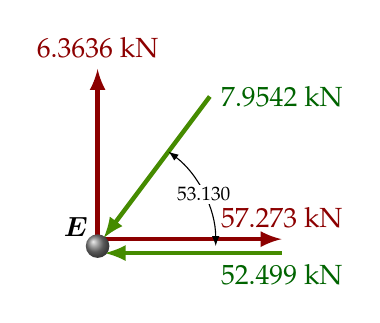
\begin{tikzpicture}[scale=\scale]

  \coordinate (E) at (0,0);
  % \footnotesize
  \draw[ultra thick, latex-, Chartreuse4] ($ (E)+(53.13:0.125cm) $) -- +(53.13:2.25cm) node[DarkGreen, right] {$7.9542\text{ kN}$} ;
  \draw[ultra thick, latex-, Chartreuse4] ($ (E)+(-45:0.125cm) $) -- +(0:2.25cm)node[DarkGreen, below] {$52.499\text{ kN}$} ;
  \draw[saitMaroon,ultra thick, -latex] (E) -- (90:2.25cm) node[ above] {$6.3636\text{ kN}$};
  \draw[saitMaroon,ultra thick, -latex]  ($ (E)+(45:0.125cm) $) -- +(0:2.25cm) node[above] {$57.273\text{ kN}$};

  \shade [ball color = gray] (E) circle (0.15cm) node[above left] {$\bm E$};


  \footnotesize
  \draw[arrows={Latex[scale=0.75]-Latex[scale=0.75]}] ($ (E)+(1.5,0) $)  arc (0:53.13:1.5cm) node[fill=white, inner sep = 0.125em] at ($ (E)+(26:1.5) $) {\scriptsize $53.130\degree$};

\end{tikzpicture}

% 					}
% 					\hfill
% 					\mini[0.5]{
% 						\begin{align*}
% 							\Sigma F_x & = 57.273-52.499                               \\
% 							           & \qquad-7.9542\cos 53.130\degree               \\
% 							           & = 0.0014686                                   \\
% 							           & \approx 0 \qquad\textcolor{green}{\checkmark} \\
% 							\Sigma F_y & =6.3636-7.9542\sin 53.130\degree              \\
% 							           & = 0.00024853\,\text{kN}                       \\
% 							           & \approx 0\qquad\textcolor{green}{\checkmark}
% 						\end{align*}
% 					}
% 					\vspace{-1cm}
% 				}
% 			\end{statsbox}
% 		\end{textblock*}
% 	}


% \end{frame}

%%%%%%%%%%%%%%%%%%%%%%%%%%%%%%%%%%%%%%%%%%%%%%%%%%%%%%%%%%%%%%%%



\begin{frame}{}
	\begin{myexer}{}{}
		\def\scale{0.65}
		\centering
		%%%%%%%%%%%%%%%%%%%%%%% TRUSS %%%%%%%%%%%%%%%%%%%%%%%%%%%%%%%%%%%%%%%%%%%%%%%%%%%%%%%%%%%%%%%%%%%%%
% !TEX root = ../../Beamer/07MoJ/07MoJd.tex

%http://tex.stackexchange.com/questions/33703/extract-x-y-coordinate-of-an-arbitrary-point-in-tikz
\makeatletter
\providecommand{\gettikzxy}[3]{%
	\tikz@scan@one@point\pgfutil@firstofone#1\relax
	\edef#2{\the\pgf@x}%
	\edef#3{\the\pgf@y}%
}
\makeatother

%%%%%%%%%%%%%%%%%%%%%%% TRUSS %%%%%%%%%%%%%%%%%%%%%%%%%%%%%%%%%%%%%%%%%%%%%%%%%%%%%%%%%%%%%%%%%%%%%


%%%%%%%%%%%%%%%%%%%%%%% TRUSS %%%%%%%%%%%%%%%%%%%%%%%%%%%%%%%%%%%%%%%%%%%%%%%%%%%%%%%%%%%%%%%%%%%%%
\begin{tikzpicture}[scale=\scale]

	\coordinate (A) at (0,0);
	\coordinate (B)	at (3,0);
	\coordinate (C) at (6,0);
	\coordinate (D) at (9,0);
	\coordinate (E) at (6,3.5);
	\coordinate (F) at (3,3.5);
	\coordinate (G) at (0,3.5);

	\fill[right color=Honeydew4,left color=Honeydew2] ($(A)+(-0.5,-3)$)rectangle($(G)+(-1.5,1)$);
	\PinnedConnection[-90]{G}{Honeydew3}{black}{0.5}{0.125}
	\PinnedConnection[-90]{A}{Honeydew3}{black}{0.5}{0.125}

	\footnotesize
	% \filldraw[fill=Cornsilk2] ($(DD)+(25:2.5)$)--++(205:2.5)--+(2.25,0);
	% \draw[latex-latex] ($(DD)+(25:1.75)$)arc(25:0:1.75)node[fill=Cornsilk2, midway, inner sep=0.5mm]{$25\degree$};

	% \fill[top color=Honeydew4,bottom color=Honeydew2] ($(G)+(-1,-0.5)$)rectangle($(G)+(1,-1)$);
	% \draw ($(A)+(-1,-0.5)$)--($(A)+(1,-0.5)$);
	% \draw ($(G)+(-1,-0.5)$)--($(G)+(1,-0.5)$);

	\pgfoonew \CF=new rrect(C,F,DarkOliveGreen4,DarkOliveGreen3,black,0.3,0.3,0.3,0.125);
	\pgfoonew \AF=new rrect(A,F,DarkOliveGreen4,DarkOliveGreen3,black,0.3,0.3,0.3,0.125);
	\pgfoonew \AB=new rrect(A,B,DarkOliveGreen4,DarkOliveGreen3,black,0.3,0.3,0.3,0.125);
	\pgfoonew \BC=new rrect(B,C,DarkOliveGreen4,DarkOliveGreen3,black,0.3,0.3,0.3,0.125);
	\pgfoonew \CD=new rrect(C,D,DarkOliveGreen4,DarkOliveGreen3,black,0.3,0.3,0.3,0.125);
	\pgfoonew \DE=new rrect(E,D,DarkOliveGreen4,DarkOliveGreen3,black,0.3,0.3,0.3,0.125);
	\pgfoonew \EF=new rrect(E,F,DarkOliveGreen4,DarkOliveGreen3,black,0.3,0.3,0.3,0.125);
	\pgfoonew \FG=new rrect(G,F,DarkOliveGreen4,DarkOliveGreen3,black,0.3,0.3,0.3,0.125);
	\pgfoonew \BF=new rrect(B,F,DarkOliveGreen4,DarkOliveGreen3,black,0.3,0.3,0.3,0.125);
	\pgfoonew \CE=new rrect(C,E,DarkOliveGreen4,DarkOliveGreen3,black,0.3,0.3,0.3,0.125);

	\draw[ultra thick, saitMaroon, -Latex] (D)--+(0,-2.75)node[below,black]{$12.0\,$kN};
	\draw[ultra thick, saitMaroon, -Latex] (C)--+(0,-2.25)node[below,black]{$10.0\,$kN};
	% \draw[ultra thick, saitMaroon, -Latex] (E)--+(0,-2.25)node[below,black]{$10.0\,$kN};
	% \draw[ultra thick, saitDeepBlue, -Latex] (A)--+(2,0)node[right,black]{$2.00\,$kN};
	%
	\shadedraw[ball color=Honeydew3, draw=black] (A) circle (2.5pt)node[xshift=0.2cm, yshift=-0.25cm]{ $A$};
	\shadedraw[ball color=Honeydew3, draw=black] (B) circle (2.5pt)node[xshift=0.2cm, yshift=-0.25cm]{ $B$};
	\shadedraw[ball color=Honeydew3, draw=black] (C) circle (2.5pt)node[xshift=0.2cm, yshift=-0.25cm]{ $C$};
	\shadedraw[ball color=Honeydew3, draw=black] (D) circle (2.5pt)node[xshift=0.2cm, yshift=-0.25cm]{ $D$};
	\shadedraw[ball color=Honeydew3, draw=black] (E) circle (2.5pt)node[yshift=0.25cm]{ $E$};
	\shadedraw[ball color=Honeydew3, draw=black] (F) circle (2.5pt)node[yshift=0.25cm]{ $F$};
	\shadedraw[ball color=Honeydew3, draw=black] (G) circle (2.5pt)node[yshift=0.25cm]{ $G$};

	\draw[thin] ($(A)+(0,-0.25)$)--+(0,-1);
	\draw[thin] ($(B)+(0,-0.25)$)--+(0,-1);
	\draw[thin] ($(D)+(0.5,0)$)--+(1,0);
	\draw[thin] ($(E)+(0.5,0)$)--+(4,0);


	\draw[latex-latex] ($(A)+(0,-1)$)--node[fill=white,inner sep=0.25mm]{$1.65\,$m}($(B)+(0,-1)$);
	\draw[latex-latex] ($(B)+(0,-1)$)--node[fill=white,inner sep=0.25mm]{$1.65\,$m}($(C)+(0,-1)$);
	\draw[latex-latex] ($(C)+(0,-1)$)--node[fill=white,inner sep=0.25mm]{$1.65\,$m}($(D)+(0,-1)$);
	\draw[latex-latex] ($(D)+(1,0)$)--node[fill=white,inner sep=0.5mm]{$2.10\,$m}($(E)+(4,0)$);

\end{tikzpicture}

		\cmini[0.65]{
			\centering
			Determine the force in each truss member.
		}
	\end{myexer}
\end{frame}


%%%%%%%%%%%%%%%%%%%%%%%%%%%%%%%%%%%%%%%%%%%%%%%%%%%%%%%%%%%%%%%%%%%%%%%%%%%%%%%%

\end{document}